%\documentclass[10pt,DIVcalc]{scrartcl}%brav, DIV berechnen lassen
%\documentclass[10pt,DIV12]{scrbook}%boese, selber am DIVrumspielen %vorher war 13
\documentclass[physics,phd,nolot,nolof]{uccthesis}%ucc thesis class, doc see ~/texmf
\usepackage{graphicx,color}
\usepackage{amsmath,amsthm, amssymb, latexsym}
\usepackage[english]{babel}
\usepackage{pdflscape}
%The following packages are commentend out because they are already loaded
%by the uccthesis class
%\usepackage[latin1]{inputenc}              
%\usepackage[numbers]{natbib}%Bibtex style file
%\usepackage{url}%gives \url command, so I can use stuff like _ in urls without latex complaining

%%%%%%%%%%%%%%%%%%%%%%%%%%%%%%%%%%%%%%%%%%%%%%%%%%%%%%%%%%%%%%
%Macros
%%%%%%%%%%%%%%%%%%%%%%%%%%%%%%%%%%%%%%%%%%%%%%%%%%%%%%%%%%%%%%
%Brackets and averages
\newcommand{\ket}[1]{\left|#1\right\rangle}
\newcommand{\bra}[1]{\left\langle#1\right|}
\newcommand{\braket}[2]{\left\langle#1|#2\right\rangle}
\newcommand{\average}[2]{\left\langle#1\right\rangle_{#2}}
%Mathematical functions 
\newcommand{\arctanh}{\text{arctanh}}
\newcommand{\Ln}{\text{Ln}}
\newcommand{\sgn}{\text{sgn}}
\newcommand{\Sgn}{\text{Sgn}}
%Alerts, important for draft
\newcommand{\alert}[1]{\textbf{\color{red}#1}}
%Integrals with the differential at the integral sign
\usepackage{twoopt}
\newcommandtwoopt{\intd}[3][][]{\int\limits_{#1}^{#2}\!\mathrm{d}#3\,}

%%%%%%%%%%%%%%%%%%%%%%%%%%%%%%%%%%%%%%%%%%%%%%%%%%%%%%%%%%%
%Graphics path
%%%%%%%%%%%%%%%%%%%%%%%%%%%%%%%%%%%%%%%%%%%%%%%%%%%%%%%%%%%
%\graphicspath{{/Pictures}{.}}
\graphicspath{{../../../Pictures/}{~/Pictures/}{./talk/}{./plots/}{}}
\DeclareGraphicsExtensions{%
.pdf,.PDF,%
.png,.PNG,%
.jpg,.mps,.jpeg,.JPEG,.JPG}

%%%%%%%%%%%%%%%%%%%%%%%%%%%%%%%%%%%%%%%%%%%%%%%%%%%%%%%%%%%
%titlepage settings
%%%%%%%%%%%%%%%%%%%%%%%%%%%%%%%%%%%%%%%%%%%%%%%%%%%%%%%%%%%
\author{Anna Hauber}
\title{
	Landau Damping and Screening 
	%\includegraphics{MOS_TEM.png}
}
\subtitle{DRAFT}

\date{\today}

%%%%%%%%%%%%%%%%%%%%%%%%%%%%%%%%%%%%%%%%%%%%%%%%%%%%%%%%%%%%
%Start of the actual document
%%%%%%%%%%%%%%%%%%%%%%%%%%%%%%%%%%%%%%%%%%%%%%%%%%%%%%%%%%%%
\begin{document}
%\maketitle 
%\thispagestyle{empty}
%\newpage
%\tableofcontents
%\newpage
%%%%%%%%%%%%%%%%%%%%%%
\chapter{Landau damping}
\alert{Background of the entire problem
interface phonon plasmon scattering problem
Start with schematic description from the progress review}
Overview\cite{boydsanderson,bittencourtplasmafundamentals}:
\begin{itemize}
  \item Kinetic theory
  \item Heuristic explanation
  \item	 Explain what collisionless means to a plasma physicist, and what the equivalent processes are in condensed matter speak, i.e. plasmons and quasiparticles interaction 
\end{itemize}
\section{Vlasov-Poisson formalism}
\subsection{Landau's article}
Let us  consider a slightly disturbed plasma.
The perturbation $f_1(\vec r, \vec v, t)$ is small compared to the equillibrium distribution function
$f_0(\vec v)$. 
The Vlasov equation 
\begin{equation}
	\frac{\partial f}{\partial t}+
	\vec{v}\cdot\frac{\partial f}{\partial \vec{r}} +
	\frac{\vec F}{m} \cdot \frac{\partial f}{\partial \vec v} 
	=0
	\label{eq:vlasov}
\end{equation}
holds for the total distribution function
\begin{equation}
	f(\vec r, \vec v,t)=f_0(\vec v)+f_1(\vec r, \vec v, t),
	\label{eq:distributionf}
\end{equation} and can be written as
\begin{equation}
	\frac{\partial f_1}{\partial t}+
	\vec{v}\cdot\frac{\partial f_1}{\partial \vec{r}} +
	\frac{\vec F}{m} \cdot \left( \frac{\partial f_0}{\partial \vec v} +
\frac{\partial f_1}{\partial \vec v} \right)
	=0.
	\label{eq:vlasov2}
\end{equation}
Hence, the Vlasov equation is equivalent to a Boltzmann equation without collision terms.

We assume a homogeneous ion distribution. In solid state physics this is often called a jellium model. 
The equilibrium electronic charge $e\intd{\vec v} f_0(\vec v)$ cancels out the background ionic charge $|e|NZ$, so that the plasma is neutral in the absence of perturbations.

In general $\vec F $ includes both external fields, and the self-consistent fields of electrons and ions in the plasma.
In our case $\vec F=e \vec E$ is only the self-consistent field due to a small perturbation of the electrons. 
Gauss's law 
\begin{equation}
\nabla\cdot \vec E(\vec r,t) = 4\pi\rho(\vec r,t)
=4\pi e\intd{\vec v}f_1(\vec r, \vec v,t)
	\label{eq:gausslaw}
\end{equation}
provides the connection between $f_1$ and $\vec E$, and tells us that $\vec E$ is also a perturbation of the order of $f_1$. 
That means that the last term in the Vlasov equation~(\ref{eq:vlasov2}) is of second order in the perturbation, so that the linearized Vlasov equation reads
	\begin{equation}
	\frac{\partial f_1}{\partial t}+
	\vec{v}\cdot\frac{\partial f_1}{\partial \vec{r}} +
	\frac{e \vec E}{m} \cdot \frac{\partial f_0}{\partial \vec v} 
	=0.
	\label{eq:vlasovlin}
\end{equation}
The scenario described has been called a ``Vlasov-Poisson'' model, for example in the review article~\cite{howtomodelqmplasmas}; this becomes more obvious if one uses the electrostatic potential $\varphi$ such that 
\begin{equation}
	\vec E=-\nabla \varphi
	\label{eq:defpotenatial}
\end{equation}
in equation (\ref{eq:vlasovlin}) and (\ref{eq:gausslaw}).

Vlasov did not solve his own equation as an initial value problem.~\cite{vlasov} 
Only Landau solved the linearized Vlasov equation as an initial value problem, found damped vibrations, and gloated that ``most of [Vlasov's previous undamped] results turn out to be incorrect''~\cite{Landaudamping1946}.

\subsubsection{Initial value problem}
This discussion follows Landau's original paper\cite{Landaudamping1946} quite closely. Some additional explainations are taken from \cite{caltechbook},\cite{boydsanderson} and \cite{bittencourtplasmafundamentals}.
Landau considered how a small perturbation that was turned on at $t=0$ evolves. 
To that end he took the Fourier transform in position of the  Vlasov-poisson-equations 
\begin{eqnarray}
	\frac{\partial f_{1,\vec k}}{\partial t} +
	i\vec{v}\cdot\vec{k} f_{1,\vec k} 
	-\frac{e \nabla \varphi_{\vec k}}{m} \cdot \frac{\partial f_0}{\partial \vec v} =0\\
	k^2\varphi_{\vec k}=4\pi e\intd{\vec v}f_{1,\vec k}(\vec v)
	\label{eq:fouriervlasov}
\end{eqnarray}
and the Laplace transform 
\begin{equation}
  g_p=\intd[0][\infty]{t} e^{-pt}g(t) \;\;\; p\in \mathbb{C}, 
	\label{eq:laplace}
\end{equation}
in time. 
The Laplace transform, as a one-sided transform, is well suited for initial value problems, and the Laplace transform of a derivative  
\begin{equation}
  \intd[0][\infty]{t} e^{-pt}\frac{d g(t)}{d t}=p g_p -g(0)
	\label{eq:laplacediff}
\end{equation}
features the value of the function g at the time $t=0$.

In order to make the following equations more reader-friendly, we drop the index $\vec k$, and we set $\vec k=k\vec e_z$ without loss of generality.
The Laplace-transformed Vlasov-Poisson equations read
\begin{eqnarray}
	(p+ikv_z)f_{1,p} -ik\frac{e}{m}\varphi_p \frac{\partial f_0}{\partial v_z}=f_{1,t=0}\\
	k^2\varphi_p=4\pi e \intd{\vec v} f_{1,p}(\vec v).
	\label{eq:laplacevlasov}
\end{eqnarray}
The first equation can be solved for $f_{1,p}$, and plugged into the second equation. 
This yields
\begin{equation}
  \varphi_p=\frac{4\pi e}{k^2} \frac{\intd{\vec v} \frac{f_{1,t=0}(\vec v)}{p+ikv_z}}
  {1-\frac{4\pi i e^2}{k m} \int d{\vec v} \frac{\partial f_0(\vec v)\partial v_z}{p+ikv_z}}.
	\label{eq:landau-potential}
\end{equation}
To illustrate that the problem is essentially longitudinal, the integrations along the $v_x$ and $v_y$ can already be carried out. 
Defining 
\begin{eqnarray}
  F_0(v_z)=	&\intd[0][\infty]{v_x} \intd[0][\infty]{v_y} f_0(\vec v) \\
  F_{1,t=0}(v_z)=	&\intd[0][\infty]{v_x} \intd[0][\infty]{v_y} f_{1}(t=0,\vec v) 
	\label{eq:abbrF}
\end{eqnarray}
the previous expression for $\varphi_p$ becomes
\begin{equation}
  \varphi_p=\frac{4\pi e}{k^2} \frac{\intd{v_z} \frac{F_{1,t=0}(v_z)}{p+ikv_z}}
	{1-\frac{4\pi i e^2}{k m} \intd v \frac{\partial F_0(v_z)\partial v_z}{p+ikv_z}}.
	\label{eq:landau-potential-F}
\end{equation}
The denominator of this is
\begin{equation}
\varepsilon(k,p)=1-\frac{4\pi e^2}{m k^2}
\int_{-\infty}^{\infty}\frac{\mathrm{d} v}{v-ipk}\frac{\partial F_0(v)}{\partial v},
	\label{eq:eps}
\end{equation}
the dielectric function of the plasma. 

Finally, the time dependence of the potential can be determined using the inverse Laplace transform 
\begin{equation}
	\varphi(t)=\frac{1}{2\pi i}\intd[\sigma-i\infty][\sigma+i\infty]p \varphi_p e^{pt}, \;\;\;\sigma>p_{max} \text{ and } \sigma>0
	\label{eq:inverselaplace}
\end{equation}
where the integration path is defined as a line parallel to the imaginary p-axis in the right half plane, which must lie to the right of all the poles $p_n$ of $\varphi_p$ to ensure convergence.

That means that p in the expressions for $\varphi_p$ and $\varepsilon_p$ above is positive, or, equivalently, that the singular point in the integrands in those expressions, $v=i\frac{p}{k}$ lies in the upper half plane, see fig.~\ref{fig:landaucontourplus}.
As the velocity integration goes along the real axis, i.e., always below the singular point, the integrands in eq~(\ref{eq:landau-potential-F})  will never be singular. 
\begin{figure}[ht]
	\begin{center}
\includegraphics[width=.75\textwidth]{plus.pdf}
	\end{center}
	\caption{Landau contour $\Gamma_L$ for $\gamma>0$ }
	\label{fig:landaucontourplus}
\end{figure}

The potential $\varphi(t)$ can be expressed in a neat way if $\varphi_p e^{pt}$ is an analytic function to the left of the line $\sigma$ except for isolated poles (meromorphic).
That means that we can use the residue theorem to express $\varphi(t)$ as
\begin{equation}
	\varphi(t)=\sum_n \text{Res}\left(\varphi_p e^{pt},p_n\right),
	\label{eq:potentialresidue}
\end{equation}
while we have to show that the integral along the path that closes the contour vanishes, see fig.~\ref{fig:jordan}. (Write about Jordan's Lemma!)
\begin{figure}[h]
	\begin{center}
	\includegraphics[width=.75\textwidth]{Jordan.pdf}
	\end{center}
	\caption{Integration path in eq.~(\ref{eq:inverselaplace}) goes along $\Gamma_\sigma$. For expression~(\ref{eq:potentialresidue}) to hold, the integral along $\Gamma_R$ in the limit $R\rightarrow\infty$ needs to vanish, see Jordan's lemma.}
	\label{fig:jordan}
\end{figure}

However, for $\varphi_p$ to be meromorphic, we have to analytically continue the integrals  of the form
\begin{equation}
	\intd[-\infty][\infty]v \frac{g(v)}{v-ipk}
	\label{eq:realaxiscontour}
\end{equation}
in eq~(\ref{eq:landau-potential-F}) into the left half plane, $\mathfrak{R}(p)<=\sigma$.
That means that the pole in the integrand in eq.~(\ref{eq:realaxiscontour}), $v_0=ipk$ can move into the lower half plane $\mathfrak{I}(v)<=0$.
That means that when you consider the integral as a function of $ipk$, it can have a discontinuity at the real axis, because the integration goes across the pole. 
Landau's approach to analytic continuation is to distort the integration path down from the real axis if necessary to avoid crossing the real axis, see fig.~\ref{fig:landaucontour}.
\begin{figure}[h]
	\begin{center}
\includegraphics[width=.75\textwidth]{plus.pdf}\\
\includegraphics[width=.75\textwidth]{null.pdf}\\
\includegraphics[width=.75\textwidth]{minus.pdf}
	\end{center}
	\caption{Landau contour $\Gamma_L$ for $\gamma$ positive, zero or negative.}
	\label{fig:landaucontour}
\end{figure}

We can use the Cauchy integral theorem to calculate the difference between the integration along the real axis and this ``Landau-contour'':\\
Consider an integration along the contour as in fig.~\ref{fig:residue}, only with the contours closed at~$\pm \infty$.
\begin{figure}[h]
	\begin{center}
	\includegraphics[width=.75\textwidth]{residue.pdf}
	\end{center}
	\caption{Integration path above and below the pole, infinitesimally close to each other. If the contour is closed, the integral along this contour yields $2\pi i $ times the residue of the integrand at the pole.}
	\label{fig:residue}
\end{figure}
If g(v) is an analytic function,
\begin{equation}
  \intd[\Gamma_L]{v} \frac{g(v)}{v-ipk}
 -\intd[\Gamma_R]v \frac{g(v)}{v-ipk}=2\pi i \text{Res}\left(\frac{g(v)}{v-ipk},ip/k\right)
	\label{eq:contourexplanation}
\end{equation}
for $\varepsilon\rightarrow0$ gives the difference between the integral evaluated at a contour that runs below the singularity, and one that runs above it along the real axis.
If the pole is above the real axis, the two are the same. If the pole lies exactly on the real axis, the difference is exactly half of $2\pi$ times the residue. 

Figures \ref{fig:landaucontourimeps} and \ref{fig:realcontourimeps}
compare a plot of the imaginary part of the analytically continued dielectric function
\begin{equation}
\varepsilon(k,p)=1-\frac{4\pi e^2}{m k^2}
\int\limits_{\Gamma_L}\frac{\mathrm{d} v}{v-ipk}\frac{\partial F_0(v)}{\partial v}
	\label{eq:eps-Landau}
\end{equation}
to the one calculated along the real axis according to eq.~(\ref{eq:eps}), for a Maxwell distribution function.
\begin{figure}[h]
	\begin{center}
	\includegraphics[width=\textwidth]{landau.pdf}
	\end{center}
	\caption{Imaginary part of the dielectric function integral evaluated along the Landau contour, for the Maxwell distribution function}
	\label{fig:landaucontourimeps}
\end{figure}
\begin{figure}[h]
	\begin{center}
	\includegraphics[width=\textwidth]{real.pdf}
	\end{center}
	\caption{Imaginary part of the dielectric function integral for the Maxwell distribution function, evaluated along the real axis}
	\label{fig:realcontourimeps}
\end{figure}

Once we have the analytic expressions for both the integrals in the expression eq.~(\ref{eq:landau-potential-F}), we can see that the poles $p_n$ that govern the time dependence of the potential $\varphi(t)$ are the zeros of the dielectric function eq.~(\ref{eq:eps-Landau}). These zeros are in general complex and wave vector dependent. 
Per construction, these zeros can only be found after the analytical continuation of $\varepsilon$. 
As $\varphi(t)$ has an exponential time dependence, $p_{max}$, the $p_k$  with the largest real part determines its long-time behaviour. 
If it is real, the  plasma oscillations are undamped. 
If it lies in the left half plane, they are damped. 
A $p_{max}$ in the right half plane corresponds to growing plasma oscillations, which, however, are not compatible with our assumption of small perturbations.
(I'm  also wondering if they are excluded by some other reason to do with the convergence of the Laplace transform. Think more later.)

\subsubsection{Longitudinal waves in a plasma}
We have seen that the zeros of the dielectric function 
determine the oscillation and expoential growth or decay of the self-consistent potential - and hence electric field in a plasma after a perturbation from equilibrium. 
Yet, we can also read
\begin{equation}
	\varepsilon(k,p)=0
	\label{eq:eps=0}
\end{equation}
as the requirement for longitudinal waves in a plasma. 

We see from eq.~(\ref{eq:eps=0}) that the frequency of these ``natural oscillations'' in general depends on wave vector.

The solution $p(k)$ to eq.~(\ref{eq:eps=0}) is complex . 
Following Landau's notation, we write
$p(k)=-i\omega(k)-\gamma(k)$, 
where $\omega$ is the frequency of the plasma oscillation.
$\gamma$, on the other hand, describes the time evolution of the amplitude of the plasma oscillation. 
If $\gamma <0$, the amplitude grows exponentially, 
if $\gamma>0$  it is damped.

\subsection{Calculation of $\varepsilon(k,p)$ in three dimensions}
The formalism above is valid for every equilibrium distribution function which is analytic as a function of the complex variable $v_z$ as desribed above. \\
It is possible to simplify the expression for the dielectric function eq.~(\ref{eq:eps-Landau}) further only using a few reasonable assumption that will be discussed below. 

We use an equilibrium distribution function $f_0$ which is normalized to the number of electrons per unit cube, 
\begin{equation}
  n_0=\intd{v} f_0(\vec v).
	\label{eq:fnormalization}
\end{equation}
Before plugging it into (\ref{eq:eps-Landau}), we have to integrate over $v_x$ and $v_y$ and differentiate with respect to $v_z$. 
It's convenient to do this in cylindrical coordinates - with  $\rho=\sqrt{v_x^2+v_y^2}$ and $z=v_z$:
\begin{equation}
  \frac{d F_0(z)}{d z}
  =\frac{\partial }{\partial z} \intd[0][2\pi]{\varphi}\intd[0][\infty]{\rho} \rho f_0(\sqrt{\rho^2 +z^2}) 
  =2\pi \frac{\partial }{\partial z}\intd[0][\infty]{\rho} \rho f_0(\sqrt{\rho^2 +z^2}) 
	\label{eq:cyclindricalcoordinatesdF}
\end{equation}
where we have used that $f_0(\vec v)=f_0(v)$.
Now we can use a result from real analysis, namely that if $ f_0(\sqrt{\rho^2 +z^2})$ is uniformly convergent,
we can exchange the order of the differentiation and the integration in eq.~(\ref{eq:cyclindricalcoordinatesdF}).~%
\footnote{Physicst usually don't worry about uniform convergence of expressions as the Maxwell-Boltzmann distribution function, which are essentially Gaussians.}
Hence, we can continue to equate 
\begin{equation}
	\begin{split}
	\frac{d F_0(z)}{d z}
	&=2\pi \intd[0][\infty]\rho\rho\frac{\partial}{\partial z}f_0(\sqrt{\rho^2 +z^2})\\ 
	&=2\pi z \intd[0][\infty]\rho\frac{\partial}{\partial \rho}f_0(\sqrt{\rho^2 +z^2}) 
	\end{split}
	\label{eq:cyclindricalcoordinatesdF2}
\end{equation}
having used $\frac{\partial f_0}{\partial z}=\frac{\partial f_0}{\partial v} \frac{\partial v}{\partial z}=\frac{\partial f_0}{\partial \rho}\frac{\partial v}{\partial z} \left(\frac{\partial v}{\partial \rho}\right)^{-1}$.
Under the additional assumption that $\lim\limits_{v\to\infty} f_0(v)= 0$, this provides us with the formula 
\begin{equation}
	\frac{d F_0(z)}{d z}=-2\pi z f_0(|z|).
	\label{eq:cyclindricalcoordinatesdF3}
\end{equation}
It will prove handy to introduce
\begin{equation}
	\omega_p=\sqrt{\frac{4\pi e^2 n_0}{m}},
	\label{eq:wp}
\end{equation} 
a characteristic frequency of the plasma, which will turn out to be the long-wavelength limit of the plasma frequency,
and is often just called the plasma frequency.~%
\footnote{Note that we use cgs units.}
This provides us with the expression
\begin{equation}
\varepsilon(k,p)=1+\frac{2\pi\omega_p^2}{n_0 k^2}
\intd[\Gamma_L]z\frac{z f_0(|z|)}{z-ipk},
\label{eq:eps-Landau-2}
\end{equation}
into which we can just plug in different equilibrium distribution functions $f_0(v)$.
%%%%%%%%%%%%%%%%%%%%%%%%%%%%%%%%%%%%%%%%%%%%%%%%%%%%%%%%%%%%%%%%%%%%%%
\subsection{Maxwell - Boltzmann distribution function}
In the following section, we will calculate the dieelectric function eq.~(\ref{eq:eps-Landau-2}), 
where $f_0(v)$ is the Maxwell-Boltzmann distribution function. 
That's the distribution function that Landau had in mind originally,
and it's applicable for a large parameter space in classical plasma physics,
where temperatures are usually high and electron densities small, see fig.~\ref{fig:plasmaregimes}.\\
\begin{figure}[ht]
	\begin{center}
	\includegraphics[width=\textwidth]{plasma-regimes+caption.png}
	\end{center}%
	\caption{Various examples for plasmas in the density n- temperature T parameter space.
	The black line divides the classical from the quantum regime. Within those sections, the green line devides the collisional sections from the non-collisional ones. 
	This leaves us with a classical non-collisional section, marked VLASOV, a classical collisional marked BOLTZMANN, the quanum non-collisional one marked WIGNER, and, finally, the quantum collisional one refferred to as WIGNER(+coll.). Room temperatur is at roughly $\log_{10}300\approx2.5$, while semiconductur carrier densities vary widely with doping. 
	From \cite{howtomodelqmplasmas}}
	\label{fig:plasmaregimes}
\end{figure}
It is easy to see that the Maxwell - Boltzmann distribution function 
\begin{equation}
	f_0(\vec v)=n_0 \left( \frac{m}{2\pi k_B T}\right)^{\frac{3}{2}}~e^{-\frac{mv^2}{2k_BT}}
	\label{eq:fMB}
\end{equation}
fullfils all the requirements to derive eq.~(\ref{eq:eps-Landau-2}). 
It turns out that the dielectric function takes a compact form if we use the  Debye length 
\begin{equation}
	\lambda_D=\sqrt{\frac{k_BT}{4\pi n_0 e^2}}
	\label{eq:Debye-length}
\end{equation}
as a length scale.
We find
\begin{equation}
	\varepsilon(k,p)=1+\frac{1}{\sqrt{2\pi}(k\lambda_D)^2}\intd[\Gamma_L]u\frac{u e^{-\frac{u^2}{2}}}{u-\frac{ip}{\omega_p}\frac{1}{k \lambda_D}},
	\label{eq:epsMB}
\end{equation}
which we will make still more legible by introducing the dimensionless wave vector
$K=k\lambda_D$ and the dimensionless frequency
$W=\frac{ip}{\omega_p}$:
\begin{equation}
	\varepsilon(K,W)=1+\frac{1}{\sqrt{2\pi}K^2}\intd[\Gamma_L]u \frac{u e^{-\frac{u^2}{2}}}{u-\frac{W}{K}}
	\label{eq:epsMBKW}
\end{equation}

Next, we have to shift our focus to the integration path $\Gamma_L$, see fig.~\ref{fig:landaucontour}.
As discussed above, integrating along the Landau contour $\Gamma_L$ is a way of finding the analytic continuation of 
\begin{equation}
	\varepsilon(K,W)=1+\frac{1}{\sqrt{2\pi}K^2}\intd[-\infty][\infty]u \frac{u e^{-\frac{u^2}{2}}}{u-\frac{W}{K}}
	\label{eq:epsMBKW-real}
\end{equation}
from the upper half plane $\mathfrak{Im}\frac{W}{K} >0$ into the lower half plane $\mathfrak{Im}\frac{W}{K}<0$.
If one just evaluates eq.~(\ref{eq:epsMBKW-real}) for all $\mathfrak{Im}\frac{W}{K}$, the resulting function will not be analytic at the real axis, see fig.~\ref{fig:realcontourimeps}.

We also described above how the contribution to the integral from the part of the Landau contour that passes below the pole $\mathfrak{Im}\frac{W}{K}<0$ is 
\begin{equation}
	2\pi i~\text{Res}\left(u e^{-\frac{u^2}{2}},\frac{W}{K}\right)
	=2\pi i\frac{W}{K} e^{-\frac{1}{2}\frac{W^2}{K^2}}
	\label{eq:ResMB}
\end{equation}

In the following, we will refrain from giving a full evalution of $\varepsilon(K,W)$, as it includes a piecewise expressions for positive, zero and negative imaginary part of $\frac{W}{K}$, because it would be awkward. 
We will only evaluate the expression for $\mathfrak{Im}\frac{W}{K}<0$, i.e.,
\begin{equation}
	\begin{split}
	\varepsilon(K,W)
	&=1+\frac{1}{\sqrt{2\pi}K^2}\left[\intd[-\infty][\infty]u \frac{u e^{-\frac{u^2}{2}}}{u-\frac{W}{K}}
	+ 2\pi i~\text{Res}\left(u e^{-\frac{u^2}{2}},\frac{W}{K}\right)\right]\\
	&=1+\frac{1}{\sqrt{2\pi}K^2}\left(\intd[-\infty][\infty]u \frac{u e^{-\frac{u^2}{2}}}{u-\frac{W}{K}}
	+2\pi i\frac{W}{K} e^{-\frac{1}{2}\frac{W^2}{K^2}}\right).
	\end{split}
	\label{eq:epsMBKW-landau}
\end{equation}
This expression is perfectly ready to be evaluted numerically now. As it happens, however, the integral in eq.~(\ref{eq:epsMBKW-landau}) can calculated, i.e., it can be transformed into an expression involving the imaginary error function
\footnote{A good account of a very similar calculation can be found in \cite{bittencourtplasmafundamentals}- the main difference is that they use the Dawson function, which is closely related to the imaginary error function.}
$\text{erfi}(z)=\frac{2}{\sqrt{\pi}}\intd[0][\infty]t e^{-t^2}$, which is well tabulated.
Using
\begin{equation}
	\intd[-\infty][\infty]u \frac{u e^{-\frac{u^2}{2}}}{u-\frac{W}{K}}
	=\sqrt{2\pi}-\pi\frac{W}{K}~e^{-\frac{1}{2}\frac{W^2}{K^2}}\left(i+\text{erfi}(\frac{W}{\sqrt{2}K}) \right)
	\label{eq:erfiint}
\end{equation}
yields 
\begin{equation}
	\varepsilon(K,W)=
	1+\frac{1}{K^2}\left\{
	1+\sqrt{\frac{\pi}{2}}\frac{W}{k}e^{-\frac{1}{2}\frac{W^2}{K^2}}
	\left[i-\text{erfi}(\frac{W}{\sqrt{2}K})\right]
	\right\} \text{ for }\mathfrak{Im}\frac{W}{K}<0.
	\label{eq:epsMBfinal}
\end{equation}
Its imaginary part is plotted in fig.~\ref{fig:landaucontourimeps}. 
The two plots in fig.~\ref{fig:landaucontourimeps} and fig.~\ref{fig:realcontourimeps}
are identical in the upper half plane, but only if we use the Landau contour as integration path is there no discontinuity at the real axis. 
This is as good a visual evidence for a correct analytical continuation as it gets.

\paragraph*{Natural oscillation frequencies}
Landau gave approximations for the wave vector dependent plasma frequency $\omega(k)$ for small and large k, \cite{Landaudamping1946}.
We are not aware of any analytical solution of $\varepsilon(k,\omega)=0$. To the best of our knowledge, eq.~(\ref{eq:epsMBfinal}) 
cannot be solved for $\omega$ explicitly. 
Even Landau's approximate solution for large wave vectors K is only an implicit equation. 
There are some variations of those approximations in textbooks, e.g.,\cite{boydsanderson} for the small k approximation of $\gamma$, and \cite{bittencourtplasmafundamentals} for a good treatment of approximations for $\omega$ for small and intermediate wave vectors, but we will constrain ourselves to Landau's ones. 
\begin{figure}[h]
	\begin{center}
	\includegraphics[width=\textwidth]{approx.pdf}
	\end{center}
	\caption{Numerically calculated $\omega(k)$ or $\gamma(k)$, and Landau's short and long - wavelenght approximations}
	\label{fig:approxomegagamma}
\end{figure}
In our notation they are
\begin{eqnarray}
k\lambda_D \ll 1:\;\; 
& \omega(k)&=\omega_p(1+\frac{3}{2}(k\lambda_D)^2)\\
& \gamma(k)&=\omega_p \sqrt{\frac{\pi}{8}}(k\lambda_D)^{-3} \text{exp}\{ -\frac{1}{2(k\lambda_D)^2}\}
	\label{eq:approxsmallk}
\end{eqnarray}
and
\begin{eqnarray}
k\lambda_D \gg 1:\;\; 
&\xi e^{\xi^22}&=\frac{(k\lambda_D)^2}{\sqrt{2\pi}} \\
& \omega(k)&=\frac{\pi}{\xi}(k\lambda_D)\\
& \gamma(k)&=\xi(k\lambda_D)\\
	\label{eq:approxbigk}
\end{eqnarray}
Figure~\ref{fig:approxomegagamma} shows those approximations, together with our numerical calculations. 
We haven't been able to find benchmarks for the entire wave vector range (Probably in reference in Bittencourt's book!), but our calculations show the correct behaviour for long and short wave vectors. 

\paragraph*{Numerical method}
We calculate the real and imaginary part of $\varepsilon(K,W)$ using the C complex.h library functions. 
Our numerical calculations use a Newton-method type GNU scientific library \cite{gslsite}
routine for multivariable root finding, which doesn't require exact derivatives, but calculates them numerically.
As a Newton-type routine, the gsl root finder needs a good initial guess for the root. 
We ensure this by first discretizing along the K axis, and starting at $W=1$ for $K=0$. 
For the  mesh point $K_i$, we use the result from $K_{i-1}$ and $W_{i-1}$. 
As the imaginary error function is not implemented in C or GSL, we use the Faddeeva package\cite{Faddeevapackage}. 

\paragraph*{Discussion of results}
We find that the plasma oscillations in a Maxwell-Boltzmann distributed plasma are always, damped. 
The damping factor $\gamma$ is very small for small wave vectors, comparable to the oscillation frequency $\omega$ at intermediate wave vectors $k\lambda_D\approx 1$. 
At large wave vectors, $\gamma$ is even larger than $\omega$. 
It is worth noting that both frequency and damping factor grow monotonously and continuously. 
Hence, it is difficult to specify a maximum wave vector or cutoff $k_{max}$, such that 
waves with $k>k_{max}$ can be said to be damped out entirely.
It has been suggested \cite{boydsanderson} to set this cutoff at $\gamma(k_{max})=\omega(k_{max})$, that is, such that the damping decrement is equal to the damping decrement, which means that the amplitude of the oscillation decreases to its $e^{th}$ part during one oscillation.
This definition is obviously somewhat arbitrary.

\subsubsection{Experimental verificatin of collisionless damping}
Following Landau's predictions of collisionless damping, it was a matter of discussion whether it was a physical effect\cite{boydsanderson},
and the experimental verification of Landau damping came only 20 years later~\cite{PhysRevLett.13.184,PhysRevLett.17.175}.
%%%%%%%%%%%%%%%%%%%%%%%%%%%%%%%%%%%%%%%%%%%%%%%%%%%
\subsection{Fermi-Dirac distribution function}
It is conceivable that Landau's formalism could be extended to the quantum regime using a semiclassical approach. 
By analogy with the derivation of the Boltzmann equation used in semiconductor physics, we keep the classical equations of motion used in the derivation of eq.~(\ref{eq:eps}), but use a Fermi-Dirac distribution function rather than a classical distribution function. 

The Fermi-Dirac distribution as a function of velocity is
\begin{equation}
	f_0(v)=n_0 \left(\frac{m}{2\pi k_BT}\right)^{\frac{3}{2}}\frac{1}{\mathfrak{F}_\frac{1}{2}(\frac{E_F}{k_BT})}
	\frac{1}{1+\text{exp}(\frac{mv^2}{2k_BT}-\frac{E_F}{k_BT})}
	\label{eq:Fermi-Dirac-Distribution-function}
\end{equation}
where the Fermi-Dirach integral
\begin{equation}
	\mathfrak{F}_j(x)=\frac{1}{\Gamma(j+1)}\intd[0][\infty]t\frac{t^j}{e^{t-x}+1},\;\;\;\
	\text{with the Gamma-function }\Gamma(x), 
	\label{eq:fermidiracintegral}
\end{equation}
is important to make sure $f_o(v)$ is properly normalized according to eq.~(\ref{eq:fnormalization}).
The distribution function now depends on the Fermi-Energy $E_F$. 
Note that the Maxwell-Boltzmann distribution function is retrieved Fermi-Dirac distribution in the limit where $\frac{E_F}{k_BT}\to-\infty$.

In strict analogy to the derivation for the Maxwell-Boltzmann distribution, we can plug $f_0(v)$ into eq.~(\ref{eq:eps-Landau-2}), and find
\begin{equation}
	\varepsilon(k,p)=1+\frac{1}{\sqrt{2\pi}(k\lambda_D)^2 \mathfrak{F}_\frac{1}{2}(\frac{E_F}{k_BT})}
	\intd[\Gamma_L]u 
	\frac{u}{1+\text{exp}(\frac{u^2}{2}-\frac{E_F}{k_BT})}
	\frac{1}{u-\frac{ip}{\omega_p}\frac{1}{k \lambda_D}}
	,
	\label{eq:epsFD}
\end{equation}
which, again, goes to the Maxwell-Boltzmann expression eq.~(\ref{eq:epsMB}) in the 
$\frac{E_F}{k_BT}\to-\infty$ limit.
Using the same dimensionless wave vector as above, and the dimensionless Fermi energy $\epsilon_F$,
we abbreviate
\begin{equation}
	\varepsilon(K,W)=1+\frac{1}{\sqrt{2\pi}K^2 \mathfrak{F}_\frac{1}{2}(\epsilon_F)}
	\intd[\Gamma_L]u 
	\frac{u}{1+\text{exp}(\frac{u^2}{2}-\epsilon_F)}
	\frac{1}{u-\frac{W}{K}}
	.
	\label{eq:epsFDKW}
\end{equation}

\subsubsection{Analytic function?}
However, we brushed over some subtleties in our derivation by analogy: The assumption that $f_0(v)$ is an analytic function is not true, at least for the entire complex plane, because it has poles for
\begin{equation}
	1+\text{exp}(\frac{mv^2}{2k_BT}-\epsilon_F)=0.
	\label{eq:FDpoles}
\end{equation}
If we set $u=\sqrt{\frac{m}{k_BT}}v=u_r+iu_i$,
where $u_r$ and $u_i$ are the real and imaginary parts of the scaled complex velocity $u$,
these poles are determined by
\begin{equation}
	\begin{split}
	u_r^2-u_i^2&=2\epsilon_F\\
	u_r u_i&=(2n+1)\pi	
\text{ with } n\in\mathbb{Z}.
	\end{split}
	\label{eq:FDpoles3}
\end{equation}
The second equation is independent of the Fermi-Energy and tells us that the poles are always off the Cartesian axes. 
It describes an infinite amount of curves, but only the ones closest to the imaginary (and hence real axis), that is with $n=0$ and $n=-1$, will be relevant.\\
The fist equation is descibes a conic section. If $\epsilon_F>0$, it is a hyberbola, if $\epsilon_F<0$ it is a parabola, and $\epsilon=0$ means just $u_r^2=u_i^2$. 
This leads to the four poles per $\epsilon_F$ of
\begin{equation}
u_r=\pm\sqrt{\epsilon_F+\sqrt{\epsilon_F^2+[(2n+1)\pi]^2}} \text{ and }
u_i=\pm\frac{(2n+1)\pi}{\sqrt{\epsilon_F+\sqrt{\epsilon_F^2+[(2n+1)\pi]^2}}} 
\text{ with } n\in\mathbb{N}.
	\label{eq:FDpoles2}
\end{equation}

Despite those poles, if you retrace the derivation of $\varepsilon(k,\omega)$ above carefully, you will find that it is still valid.
%Following section is irrelavant and not particularly elucidating.
%%%%%%%%%%%%%%%%%%%%%%%%%%%%%%%%%%%%%%%%%%%%%%%%%%%%%%%%%%%%%%%%%
%Even if the poles described in eq.~(\ref{eq:FDpoles}) where lying straight between $\frac{ip}{k}$ and the real axis, the Landau contour could still be contorted such that it passes below the pole $\frac{ip}{k}$, while stayin on a domain in which $f_0(v)$ is analytic. 
%According to the residue theorem, the actual integration path inside this domain doesn't change the value of the integral.
Firstly, because the poles are off the real axis, the part of the integration that is along the real axis will not be problematic; 
secondly, because $f_0(v)$ is still analytic in the part of the half plane into which the Landau contour needs to be deformed in order to pass below the pole $\frac{ip}{k}$.
This issue would become tricky if the pole from eq.~(\ref{eq:FDpoles3}) coincided with $\frac{ip}{k}$.
However, our numerical calculations show that 
\begin{equation}
	\begin{split}
	\lim\limits_{K\to\infty}|\frac{\mathfrak{Im}(W)}{K}|= |u_i^{0}|\\
	\lim\limits_{K\to\infty}|\frac{\mathfrak{Re}(W)}{K}|= |u_r^{0}|,
\end{split}
	\label{eq:FDlimits}
\end{equation}
see fig~\ref{fig:limits},
\begin{figure}[h]
	\begin{center}
	%For path of pictures:
	%homeworkLandaudamping/Fermi/omegafirst/Ef1/newdat
	\includegraphics[width=\textwidth]{limits.pdf}
	\end{center}
	\caption{Numerical calculations for  $|\frac{\mathfrak{Im}(W)}{K}|$ and $|\frac{\mathfrak{Re}(W)}{K}|$ as functions of K. They go to $u_i^0$ and $u_r^0$ for $K\to\infty$, respectively. The calculation is for $\epsilon_F=1$}
	\label{fig:limits}
\end{figure}
and that the plasma dispersion line 
$\frac{\mathfrak{Im}(W)}{K}(\frac{\mathfrak{Re}(W)}{K})$ is always closer to the real axis otherwise, see fig.~\ref{fig:FDpoles}.
\begin{figure}[h]
	%For path of pictures:
	%homeworkLandaudamping/Fermi/omegafirst/Ef1/newdat
	\begin{center}
	\includegraphics[width=.5\textwidth]{pole.png}%
	\includegraphics[width=.5\textwidth]{pole2.png}
	\end{center}
	\caption{Plot of the imaginary (left) and real (right) parts of the integral $\intd[\Gamma_L]u \frac{u}{1+\text{exp}(\frac{u^2}{2}-\epsilon_F)} \frac{1}{u-\frac{W}{K}}$ in eq.~(\ref{eq:epsFDKW}).
	Note the position of the pole arising from the pole in the Fermi-Dirac distribution function relative to the plasma dispersion line in the $\frac{\mathfrak{Im}(W)}{K}$ -$\frac{\mathfrak{Re}(W)}{K}$ plane. The calculation is for $\epsilon_F=1$}
	\label{fig:FDpoles}
\end{figure}
This figure also shows that there is no discontinuity at the real axis. In analogy to the Maxwell-Boltzmann case discussed above, the integration along the Landau contour means that the dielectric function is continued analytically into the lower half plane.
%%%%%%%%%%%%%%%%%%%%%%%%%%%%%%%%%%%%%%%%%%%%%%%%%%%
\subsubsection{Numerical method}
We calculated the dielectric constant for several values of $\epsilon_F=\frac{E_F}{k_BT}$, corresponding to either different Fermi-Energy, i.e., electron density, or to different temperature, depending on how we interpret the quotient.

The integral along the real axis in eq.~(\ref{eq:epsFDKW}) has to be carried out numerically. 
To this end, we split it up into its real and imaginary part, and use symmetry to restrict the integration to the positive real axis.
Finally, we chop the integration domain into two. The integration over the finite domain is carried out with a simple Simpson routine.
The other one, which runs up to $\infty$ is first transformed into an integral on a finite domain as described in the chapter on improper integrals in \cite{nr} before the integration is carried out with another Simpson routine.

For the calculation of the plasma dispersion, we took advantage of the fact that the imaginary part of $\varepsilon(K,W)$ in eq.~(\ref{eq:epsFDKW}) depends only on the ration $\frac{W}{K}$, and not on either one individually.
Therefore, we can solve the equation 
\begin{equation}
	\mathfrak{Im}\{\varepsilon(\frac{W}{K})\}=0  
	\label{eq:imepszero}
\end{equation}
just by discretizing along the real part of $\frac{W}{K}$ and finding the corresponding imaginary part using a bisection routine. 
Our previous knowledge that only the solution with the largest imaginary part is relevant means that we only have to find one root. 
Now, with the imaginary part of $\frac{W}{K}$ as a function of its real part,
$\mathfrak{Im}\{\frac{W}{K}\}\left(\mathfrak{Re}\{\frac{W}{K}\}\right)$,
we can eliminate either the real of imaginary part of $W$ in the equation
\begin{equation}
	\mathfrak{Re}\{\varepsilon(K,\frac{W}{K})\}=0 . 
	\label{eq:reepszero}
\end{equation}
This is again solved with a bisection routine on a K mesh. 

\subsubsection{Results}
\begin{figure}[h]
	%Figure from 
	%homeworkLandaudamping/Fermi/omegafirst
	\begin{center}
	\includegraphics[width=\textwidth]{VPFDdebye.pdf}
	\end{center}
	\caption{Plasma dispersion for the Vlasov-Poisson equations with a Fermi-Dirac distribution function as described by the zeros of the dielectric function in eq.~(\ref{eq:epsFDKW}). The plasma dispersion lines approach the Maxwell-Boltzmann one as $\epsilon_F\to-\infty$.}
	\label{fig:plasmadispersionVPFD}
\end{figure}
The dispersion of the plasma oscillation is shown in fig.~\ref{fig:plasmadispersionVPFD}, for different $\epsilon_F$.
The case of a Maxwell-Boltzmann distribution function is also shown. 
From our calculations, we expect that we can retrieve Maxwell-Boltzmann behaviour in the limit
$\epsilon_F\to-\infty$. 
This is confirmed in this plot: The dispersion for $\epsilon_F=5$ is already hardly distinguishable from the Maxwell-Boltzmann one.

In the long wavelength limit we find an undamped plasma oscillation at frequency $\omega_P$ for all $\epsilon_F$.
At fixed nonzero wave vector, as $\epsilon_F$ grows, the frequency $\omega\omega_P$ grows, while the damping rate $\gamma\omega_P"$ decreases. 
Note, however, that the dampings stays nonzero for all nonzero wave vector, a fact which is hard to discern from the plot.
\begin{figure}[h]
	\begin{center}
	\resizebox{\textwidth}{!}{% GNUPLOT: LaTeX picture with Postscript
\begingroup
  \fontfamily{Times}%
  \selectfont
  \makeatletter
  \providecommand\color[2][]{%
    \GenericError{(gnuplot) \space\space\space\@spaces}{%
      Package color not loaded in conjunction with
      terminal option `colourtext'%
    }{See the gnuplot documentation for explanation.%
    }{Either use 'blacktext' in gnuplot or load the package
      color.sty in LaTeX.}%
    \renewcommand\color[2][]{}%
  }%
  \providecommand\includegraphics[2][]{%
    \GenericError{(gnuplot) \space\space\space\@spaces}{%
      Package graphicx or graphics not loaded%
    }{See the gnuplot documentation for explanation.%
    }{The gnuplot epslatex terminal needs graphicx.sty or graphics.sty.}%
    \renewcommand\includegraphics[2][]{}%
  }%
  \providecommand\rotatebox[2]{#2}%
  \@ifundefined{ifGPcolor}{%
    \newif\ifGPcolor
    \GPcolortrue
  }{}%
  \@ifundefined{ifGPblacktext}{%
    \newif\ifGPblacktext
    \GPblacktexttrue
  }{}%
  % define a \g@addto@macro without @ in the name:
  \let\gplgaddtomacro\g@addto@macro
  % define empty templates for all commands taking text:
  \gdef\gplbacktext{}%
  \gdef\gplfronttext{}%
  \makeatother
  \ifGPblacktext
    % no textcolor at all
    \def\colorrgb#1{}%
    \def\colorgray#1{}%
  \else
    % gray or color?
    \ifGPcolor
      \def\colorrgb#1{\color[rgb]{#1}}%
      \def\colorgray#1{\color[gray]{#1}}%
      \expandafter\def\csname LTw\endcsname{\color{white}}%
      \expandafter\def\csname LTb\endcsname{\color{black}}%
      \expandafter\def\csname LTa\endcsname{\color{black}}%
      \expandafter\def\csname LT0\endcsname{\color[rgb]{1,0,0}}%
      \expandafter\def\csname LT1\endcsname{\color[rgb]{0,1,0}}%
      \expandafter\def\csname LT2\endcsname{\color[rgb]{0,0,1}}%
      \expandafter\def\csname LT3\endcsname{\color[rgb]{1,0,1}}%
      \expandafter\def\csname LT4\endcsname{\color[rgb]{0,1,1}}%
      \expandafter\def\csname LT5\endcsname{\color[rgb]{1,1,0}}%
      \expandafter\def\csname LT6\endcsname{\color[rgb]{0,0,0}}%
      \expandafter\def\csname LT7\endcsname{\color[rgb]{1,0.3,0}}%
      \expandafter\def\csname LT8\endcsname{\color[rgb]{0.5,0.5,0.5}}%
    \else
      % gray
      \def\colorrgb#1{\color{black}}%
      \def\colorgray#1{\color[gray]{#1}}%
      \expandafter\def\csname LTw\endcsname{\color{white}}%
      \expandafter\def\csname LTb\endcsname{\color{black}}%
      \expandafter\def\csname LTa\endcsname{\color{black}}%
      \expandafter\def\csname LT0\endcsname{\color{black}}%
      \expandafter\def\csname LT1\endcsname{\color{black}}%
      \expandafter\def\csname LT2\endcsname{\color{black}}%
      \expandafter\def\csname LT3\endcsname{\color{black}}%
      \expandafter\def\csname LT4\endcsname{\color{black}}%
      \expandafter\def\csname LT5\endcsname{\color{black}}%
      \expandafter\def\csname LT6\endcsname{\color{black}}%
      \expandafter\def\csname LT7\endcsname{\color{black}}%
      \expandafter\def\csname LT8\endcsname{\color{black}}%
    \fi
  \fi
  \setlength{\unitlength}{0.0500bp}%
  \begin{picture}(7200.00,5040.00)%
    \gplgaddtomacro\gplbacktext{%
      \csname LTb\endcsname%
      \put(992,1024){\makebox(0,0)[r]{\strut{}-2}}%
      \put(992,1629){\makebox(0,0)[r]{\strut{}-1}}%
      \put(992,2234){\makebox(0,0)[r]{\strut{} 0}}%
      \put(992,2840){\makebox(0,0)[r]{\strut{} 1}}%
      \put(992,3445){\makebox(0,0)[r]{\strut{} 2}}%
      \put(992,4050){\makebox(0,0)[r]{\strut{} 3}}%
      \put(992,4655){\makebox(0,0)[r]{\strut{} 4}}%
      \put(1184,704){\makebox(0,0){\strut{} 0}}%
      \put(2504,704){\makebox(0,0){\strut{} 1}}%
      \put(3824,704){\makebox(0,0){\strut{} 2}}%
      \put(5143,704){\makebox(0,0){\strut{} 3}}%
      \put(6463,704){\makebox(0,0){\strut{} 4}}%
      \put(256,2839){\rotatebox{-270}{\makebox(0,0){\strut{} Frequency $\omega/\omega_{P}$ or damping $\gamma/\omega_{P}$}}}%
      \put(6782,2839){\rotatebox{-270}{\makebox(0,0){\strut{}}}}%
      \put(3823,224){\makebox(0,0){\strut{} Wave vector $k/k_{TF}$}}%
      \put(3823,4495){\makebox(0,0){\strut{}}}%
      \put(3823,4494){\makebox(0,0){\strut{}}}%
      \put(416,160){\makebox(0,0)[l]{\strut{}}}%
    }%
    \gplgaddtomacro\gplfronttext{%
      \csname LTb\endcsname%
      \put(5056,4432){\makebox(0,0)[r]{\strut{}$E_{F}=k_B T $: $\omega$}}%
      \csname LTb\endcsname%
      \put(5056,4112){\makebox(0,0)[r]{\strut{}		     $\gamma$}}%
      \csname LTb\endcsname%
      \put(5056,3792){\makebox(0,0)[r]{\strut{}$E_{F}=5 k_B T $: $\omega$}}%
      \csname LTb\endcsname%
      \put(5056,3472){\makebox(0,0)[r]{\strut{}		     $\gamma$}}%
      \csname LTb\endcsname%
      \put(5056,3152){\makebox(0,0)[r]{\strut{}$E_{F}=10 k_B T $: $\omega$}}%
      \csname LTb\endcsname%
      \put(5056,2832){\makebox(0,0)[r]{\strut{}		     $\gamma$}}%
      \csname LTb\endcsname%
      \put(5056,2512){\makebox(0,0)[r]{\strut{}$T=0$: $\omega$}}%
      \csname LTb\endcsname%
      \put(5056,2192){\makebox(0,0)[r]{\strut{}$T=0$: $\gamma$:}}%
      \csname LTb\endcsname%
      \put(5056,1872){\makebox(0,0)[r]{\strut{}$T=0$:  $v_{F}=\frac{\omega}{k}$}}%
    }%
    \gplbacktext
    \put(0,0){\includegraphics{plots/VPFDTF.pdf}}%
    \gplfronttext
  \end{picture}%
\endgroup
}
	\end{center}
	\caption{Plasma dispersion for the Vlasov-Poisson equations with a Fermi-Dirac distribution function as described by the zeros of the dielectric function in eq.~(\ref{eq:epsFDKW}).
	The wave vector axis is scaled with the Thomas Fermi screening length for a degenerate Fermi gas. 
	The plot shows plasma dispersions for different $\epsilon_F$ and the degenerate case is marked with $T=0$. The long wavelength behaviour for the degenerate case, i.e., $\omega=v_Fk$ is also included. Plasma oscillations in the degenerate plasma are undamped.}
	\label{fig:plasmadispersionVPFDTF}
\end{figure}

\paragraph*{Low temperature limit}
We demonstrated that our calculations show the appropriate Maxwell-Boltzmann distribution function behaviour for $\epsilon_F\to-\infty$. 
It is a natural next step to look for the behaviour in the limit where $\epsilon_F\to\infty$. 
We will understand this as the limit $T\to0$ for nonzero $E_F$, and get the degenerate Fermi-Dirac distribution function.
The results for the degenerate case are presented in the following section.
Yet, in order to compare the present results to the appropriate limit, we need to rescale the wave vector axis, which is currently temperature dependent via $\lambda_D$, to a scale that still makes sense for $T=0$. 
We can do this by using the Thomas-Fermi screening length rather than the Debye screening length as a length scale. 
It is defined as
\begin{equation}
	k_{TF}^2=4\pi e^2\frac{\partial n}{\partial E_F},
	\label{eq:KTF}
\end{equation}
see, e.g., \cite{asc87}, but we specifically use it such that
\begin{equation}
	n=\frac{1}{3\pi^2}(\frac{2m}{\hbar}E_F)^\frac{3}{2}
	\label{eq:ndegenerateFermi}
\end{equation}
which only holds exactly for degenerate Fermi gases. 
That means that what we now define as 
\begin{equation}
	k_{TF}^2=6\pi e^2 \frac{n}{E_F}
	\label{eq:Ktf}
\end{equation}
is only the Thomas-Fermi screening vector for the degenerate Fermi gas. 
For non-degenerate Fermi gases it is only a convenient length scale.
Rescaling all used equations, and even solutions is easy, because
\begin{equation}
	k_{TF}^{-1}=\sqrt{\frac{2\epsilon_F}{3}}\lambda_D,
	\label{eq:thomasfermidebye}
\end{equation}
but only makes sense if $\epsilon_F>0$.
Figure~\ref{fig:plasmadispersionVPFDTF} shows the rescaled plasma dispersions for $\epsilon_F=1$, 5 and 10, along with the one for the degenerate Fermi gas.

We can see that the dispersion lines approach the degenerate limit as $\epsilon_F$ grows.
For fixed nonzero wave vector, the damping descreases with increasing  $\epsilon_F$, but doesn't vanish exect for $k=0$.
For the degenerate case, the plasma oscillations are undamped, and their frequency approaches $\omega=v_Fk$, i.e., their phase velocity equals the Fermi velocity. 

%%%%%%%%%%%%%%%%%%%%%%%%%%%%%%%%%%%%%%%%%%%%%%%%%%%
\clearpage%This shows all the pictures before the next section starts - on a new page. 
%%%%%%%%%%%%%%%%%%%%%%%%%%%%%%%%%%%%%%%%%%%%%%%%%%%%%%%%%%%%%%%%%%
%%%%%%%%%%%%%%%%%%%%%%%%%%%%%%%%%%%%%%%%%%%%%%%%%%%%%%%%%%%%%%%%%%
\section{Wigner-Poisson}
\begin{itemize}
  \item Limitations of classical /semiclassical models
  \item Wigner formalism, see~\cite{howtomodelqmplasmas}
  \item Equivalent RPA (random phase approximation), see~\cite{pineselementary}
\end{itemize}
The random phase approximation\cite{pineselementary} and the  Wigner-Vlasov formalism\cite{howtomodelqmplasmas} both yield
 \begin{equation}
\varepsilon(k,\omega)=1-\frac{4\pi e^2}{m k^2}
\int\limits_{\Gamma_L}\frac{\mathrm{d} v}{v-\omega/k}  \frac{F_0(v+\frac{\hbar k}{2m})-F_0(v-\frac{\hbar k}{2m})}{\frac{\hbar k}{m}}.
  \label{eq:eps-wigner-poisson}
\end{equation}
It is easy to see that this equation goes back to the Vlasov-Poisson equivalent eq.~(\ref{eq:eps-Landau}) in the limit where the wave vector $k$ goes to zero.
The modified distribution function $F_0(v)$ - already defined in eq.~(\ref{eq:abbrF})- is obtained by integrating over the transverse directions:
\begin{equation}
  F_0(v_z)=\intd v_x \intd v_y f_0(\vec v)
  \label{eq:F_0}
\end{equation}
The equilibrium distribution function $f_0(\vec v)$ has to be quantum mechanical too, to be consistent with eq.~(\ref{eq:eps-wigner-poisson}),
like the Fermi-Dirac distribution function in eq.~(\ref{eq:Fermi-Dirac-Distribution-function}).
\subsection{T$>$0 case}
See \cite{finiteT-lindhard}
\subsubsection{Fermi-Dirac distribution function}
We have normalized it to the electron density, $n_0$, which we keep as a parameter. 
Note that it could be calculated explicitly as a function of the chemical potential $\mu$, and resulting in an alternative parametrization:
\begin{equation}
  \begin{split}
    n_0	&=\frac{2}{(2\pi)^3}\intd{^3\vec k} f_0(\vec k) 
 	 =\frac{8\pi}{(2\pi)^3}\intd k \frac{k^2}{1+\exp\left[(\frac{\hbar^2 k^2}{2 m}-\mu)\beta\right]} \\	
	& = \frac{\sqrt 2}{\pi^2} \left(\frac{m}{\hbar^2\beta} \right)^\frac{3}{2} \Gamma(\frac{3}{2}) \mathfrak{F}_\frac{1}{2}(\mu\beta)
 	 =2 \left( \frac{m k_B T}{2\pi\hbar^2} \right)^\frac{3}{2}\mathfrak{F}_\frac{1}{2}(\mu\beta)
  \end{split}
  \label{eq:n0-explicit}
\end{equation}
The Fermi-Dirac integrals $\mathfrak{F}_j$ are defined in eq.~(\ref{eq:fermidiracintegral}).
Thus, we could also write the distribution function as 
\begin{equation}
  f_0(\vec v)%=
%2 \left( \frac{m k_B T}{2\pi\hbar^2} \right)^\frac{3}{2}
%\left(\frac{m}{2\pi k_BT}\right)^{\frac{3}{2}}
%\frac{1}{1+\text{exp}(\frac{mv^2}{2k_BT}-\frac{E_F}{k_BT})}
=2\left(\frac{m}{2\pi\hbar}\right)^3
\frac{1}{1+\text{exp}(\frac{mv^2}{2k_BT}-\frac{\mu}{k_BT})}.
  \label{eq:Fermi-Dirac-distribution-alternativ}
\end{equation}
\subsubsection{Fermi-Energy scaling}
In order to investigate the effects of temperature on the dielectric functions, scales for  both energy and wave vector which are independent of temperature can be useful.
The Fermi energy is the chemical potential at zero temperature, and the Fermi wave vector is the corresponding wave vector:
\begin{equation}
  E_F=\frac{\hbar^2 k_F^2}{2 m}.
  \label{eq:Fermi_E_k}
\end{equation}
The Fermi wave vector $k_F$ is only determined by the density of carriers\footnote{Keep in mind that the density of carrieres changes with temperature. Hence, the comparison is between a system that has $n_0$ carriers at zero temperature, and a system that has $n_0$ carriers at nonzero temperature. Cooling down the latter system to $T=0$ would leave it with less than $n_0$ carriers in general.}
\begin{equation}
  n_0=\frac{1}{3\pi^2}k_F^3  \text{ or } k_F=\sqrt[3]{3\pi^2 n_0}
  \label{eq:Fermi_k}
\end{equation}
Using eq.~(\ref{eq:n0-explicit}), we can express how the Fermi energy is connected
to the chemical potential at a given temperature $k_BT=\frac{1}{\beta}$
\begin{equation}
  E_F\beta=\left[\frac{3\sqrt{\pi}}{4}\mathfrak{F}_\frac{1}{2}(\mu\beta) \right]^\frac{2}{3}
  =\left[\frac{3}{2}\intd[0][\infty]{x}\frac{x^\frac{1}{2}}{1+e^{x-\mu\beta}} \right]^\frac{2}{3}
  \label{eq:E_F_mu}
\end{equation}
Figure \ref{fig:Efmu} shows that the Fermi energy is positive for all chemical potentials. This makes it useful for scaling energies with it.  
\begin{figure}[ht]
  \begin{center}
    \input{Efmu.tex}
  \end{center}
  \caption{Fermi energy $E_F$ as a function of chemical potential $\mu$, both in units of the thermal energy $k_B T=\frac{1}{\beta}$.}
  \label{fig:Efmu}
\end{figure}
One can also see that for low temperatures, $\mu \gg k_B T$, $E_F \to \mu$ as desired.

We will now calculate $F_0(v_z)$, which is most easily done in cylindrical coordinates - with  $\rho=\sqrt{v_x^2+v_y^2}$ and $z=v_z$:
\begin{equation}
  \begin{split}
    F_0(z)
    &=\intd[0][2\pi]\varphi\intd[0][\infty]\rho \rho f_0(\sqrt{\rho^2 +z^2})\\
    & =\left(\frac{m}{2\pi\hbar}\right)^3 
    4\pi \intd[0][\infty]\rho  
\frac{\rho}{1+\text{exp}(\frac{m\rho^2}{2k_BT}-\frac{\mu}{k_BT}+\frac{m z^2}{2k_BT})}\\
&=\frac{4\pi m^2}{(2\pi)^3 \hbar^3\beta}\mathfrak{F}_0(\frac{\mu}{k_BT}-\frac{m z^2}{2k_BT})
  \end{split}
  \label{eq:cyclindricalcoordinatesF}
\end{equation}
We have used the Fermi-Dirac integral eq.~({\ref{eq:fermidiracintegral})
\begin{equation}
  \mathfrak{F}_0(x)=\ln (1+\exp(x)),
  \label{eq:fermi-dirac-int_0}
\end{equation}
the only one which can be expressed in closed form.

We will now try to find suitable dimensionless quantities, which enable us to write the dielectric function more simply.
There are several choices at hand. The first one is most suitable for the near degenerate limit, i.e., for $k_B T<< \mu$. 
\subsubsection{Degenerate limit parameterisation, $k_B T<< \mu$}

Next, the expression $F_0(v \pm \frac{\hbar k}{2 m})$ in the integrand of (\ref{eq:eps-wigner-poisson}) needs to be evaluated. 
The argument of $\mathfrak{F}_0$, $\beta \left[ \mu -\frac{m}{2}\left(v \pm \frac{\hbar k}{2m}\right)^2\right]
=\beta \left[ \mu - E_F\left(\frac{v}{v_F}\pm\frac{k}{2k_F}\right)^2\right]$,
once one introduces $v_F=\sqrt{\frac{2E_F}{m}}$,the Fermi velocity at nonzero temperature.

With these parameters, the dielectric function reads
\begin{equation}
  \begin{split}
  \varepsilon(k,\omega)=1-
  \frac{k_{F}^3}{k^3}\frac{1}{E_F\beta}\frac{1}{\pi k_F a_0}
  \int\limits_{\Gamma_L}\frac{\mathrm{d} u}{u-\frac{\omega}{k v_F}} 
  \left\{
   \ln\left[ 1+\exp\left(\beta\mu- \beta E_F(u+\frac{k}{2k_F})^2 \right)\right]
   \right. \\ \left.
  -\ln\left[ 1+\exp\left(\beta\mu- \beta E_F(u-\frac{k}{2k_F})^2 \right)\right]
  \right\}.
  \end{split}
  \label{eq:epsTnonzero}
\end{equation}
We have used the Bohr radius
\begin{equation}
  a_0=\frac{\hbar^2}{e^2 m}.
  \label{eq:a0}
\end{equation}
If we introduce the dimensionless prefactor 
\begin{equation}
  A=\frac{2e^2 m^2}{\pi \hbar^4 \beta k^3}=
\frac{k_{F}^3}{k^3}\frac{1}{E_F\beta}\frac{1}{\pi k_F a_0},
  \label{eq:perfactorA}
\end{equation}
wave vector
$b=\frac{k}{2k_F}$
and phase velocity
$c=\frac{\omega}{k v_F}$,
the dielectric function 
\begin{equation}
  \varepsilon = 1-A 
  \int\limits_{\Gamma_L} \frac{\mathrm{d} u}{u-c} 
  \left\lbrace
   \ln \left\{  1+\exp\left(\beta\mu- \beta E_F(u+b)^2 \right) \right\}
   -\ln \left\{ 1+\exp\left(\beta\mu- \beta E_F(u-b)^2 \right) \right\} 
  \right\rbrace
  \label{eq:epsTnonzeroshort}
\end{equation}
fits onto one line.

Note that the parameters occuring are not all independent. 
Indeed, only the temperature variable $\beta=\frac{1}{k_B T}$, 
and one of the parameters $n_0$, $\mu$, $w_p$,$E_f$ or $k_F$ can be chosen freely.
All other parameters can be derived from those two for given material constants. 

Moreover, remember that $c=c_r+ic_i$ is a complex quantity, because $\omega$ is.
%%%%%%%%%%%%%%%%%%%%%%%%%%%%%%%%%%%%%%%%%%%%%%%%%%%%%%%%%%%%%%%%
\subsubsection{Real and imaginary part  of the dielectric function}
The integration in eq.~(\ref{eq:epsTnonzero}) and eq.~(\ref{eq:epsTnonzeroshort}) is along the Landau contour $\Gamma_L$. 
\paragraph*{Residue contribution}
%%%%%%%%%%%%%%%%%%%%%%%%%%%%%%%%%%%%%%%%%%%%%%%%%%%%%%%%%%%%%%%%
The contribution from the integral along the path below the pole of the dielectric function 
eq.~(\ref{eq:epsTnonzeroshort}) at $u=c$ is
  \begin{equation}
    \varepsilon_{res}=-2\pi I \,A 
  \left\lbrace
   \ln \left\{  1+\exp\left(\beta\mu- \beta E_F(c+b)^2 \right) \right\}
   -\ln \left\{ 1+\exp\left(\beta\mu- \beta E_F(c-b)^2 \right) \right\} 
  \right\rbrace,
    \label{eq:epsTnonzero_res}
  \end{equation}
  according to the Cauchy principal formula, see above.
  This only holds if the logarithm is analytic between the real axis and and the pole $u=c$.\\
  PLOT!
  CHECK LATER!
\paragraph*{Contribution form integral along the real axis}
The contribution to the integral from the integration along the real axis has the real part
\begin{equation}
   \varepsilon_r = 1-A 
  \intd[-\infty][\infty]u
  \frac{u-c_r}{(u-c_r)^2+c_i^2} 
   \ln
   \left[
   \frac{  1+\exp\left(\beta\mu- \beta E_F(u+b)^2 \right) }
   { 1+\exp\left(\beta\mu- \beta E_F(u-b)^2 \right) } 
   \right]
  \label{eq:epsTnonzero_r}
\end{equation}
and the imaginary part
\begin{equation}
   \varepsilon_i = -A 
  \intd[-\infty][\infty]u
  \frac{c_i}{(u-c_r)^2+c_i^2} 
   \ln
   \left[
   \frac{  1+\exp\left(\beta\mu- \beta E_F(u+b)^2 \right) }
   { 1+\exp\left(\beta\mu- \beta E_F(u-b)^2 \right) } 
   \right].
  \label{eq:epsTnonzero_i}
\end{equation}
Both integrals are well-defined as long as $c$ has a non-vanishing imaginary part. 
If $c$ becomes real, $\varepsilon_i$ vanishes,
but the integrand in the real part integral has a pole at $u=c_r$.
%%%%%%%%%%%%%%%%%%%%%%%%%%%%%%%%%%%%%%%%%%%%%%%%%%%%%%%%%%%%%%%%%%%%%%%%%
\paragraph*{Evaluation of $\varepsilon_r$ for real frequencies}
Let us investigate the integral in eq.~(\ref{eq:epsTnonzero_r}) for $ci=0$ more closely.
If we introduce the integral 
\begin{equation}
  I_a(x)=\int\limits_{-\infty}^\infty \frac{\mathrm{d} u}{u} 
  \ln\left[1+\exp\left(a- E_F\beta(a)(u+x)^2 \right)\right],
  \label{eq:Int_mu_x}
\end{equation}
with the function $E_F\beta$ from eq.~(\ref{eq:E_F_mu}),
we can write
\begin{equation}
  \int\limits_{-\infty}^\infty\frac{\mathrm{d} u}{u} 
   \ln
   \left[
   \frac{  1+\exp\left(\beta\mu- \beta E_F(u+c_r+b)^2 \right) }
   { 1+\exp\left(\beta\mu- \beta E_F(u+c_r-b)^2 \right) } 
   \right]=I_{\mu\beta}(c_r+b) -I_{\mu\beta}(c_r -b).
  \label{eq:epsTnonzero_realfrequency}
\end{equation}

Hence, the real part of the dielectric function for real frequencies simply becomes 
\begin{equation}
  \varepsilon_r(k,\omega)	=
  		1-A \left[ 
		I_{\mu\beta}(c_r+b)-I_{\mu\beta}(c_r-b)
		\right].
\label{eq:reepsWingerPoisson_realw}
\end{equation}

Transforming $I_a(x)$ so that the integration is only over positive u yields
\begin{equation}
  I_a(x)=\int\limits_{0}^\infty \frac{\mathrm{d} u}{u} 
  \ln\left[
  \frac
  { 1+\exp\left(a- E_F\beta(a)(u+x)^2 \right)}
  { 1+\exp\left(a- E_F\beta(a)(u-x)^2 \right)}
  \right].
  \label{eq:Int_mu_x}
\end{equation}
It is easy to see that $I_a(x)$ is antisymmetric with respect to x.
Moreover, according to L'Hospital's rule,
\[
\lim_{u \to 0}  i_a(u,x)=\lim_{u \to 0} \frac{1}{\frac{\partial}{\partial u} u}\frac{\partial}{\partial u}  \ln\left[
  \frac
  { 1+\exp\left(a- E_F\beta(a)(u+x)^2 \right)}
  { 1+\exp\left(a- E_F\beta(a)(u-x)^2 \right)}
  \right]
  =-\frac{4E_F\beta(a)x}{ 1+\exp\left(-a +E_F\beta(a)x^2 \right)}
\]
its integrand  $i_a(u,x)$ doesn't become singular at $u=0$.

Moreover, the integrand $i_a(u,x)$ decays exponentially for large u. 
Let the Gaussian centered around x in $i_a(u,x)$ have decayed so that it's way smaller than unity - for example at $u=x+\sqrt{\frac{a+2\ln10}{E_F\beta(a)}}$, the Gaussian would have fallen off to 0.01-
a Taylor expansion of the logarithm in the integrand will yield
$i_a(u,x)\approx \frac{1}{u}\exp(a-E_F\beta(a)(u-x)^2$.
That means that tail of the integral for very large u converges.

$I_a(x)$ will have to be calculated numerically and tabulated for every $a$ and $x$. 

However, the assymtotic behaviour for large x can be calculated more easily.\\
For $x\gg1$ , $e^{-2E_F\beta(a)ux}\ll\;e^{2E_F\beta(a)ux}$, so that 
$I_a(x)\approx-\int_{0}^\infty\frac{\mathrm{d} u}{u}\ln\left[1+\exp\left(a-E_F\beta(a)(u-x)^2\right)\right]$.
If, moreover, the width of the gaussian is much smaller than x 
- say $x\gg\sqrt{\ln(10)/E_F\beta(a)}$, the width where the Gaussian has fallen off to a tenth of its peak value -
we can approximate further
\[
I_a(x)\approx-\frac{1}{x}\intd[0][\infty]u 
  \ln\left[ 1+\exp\left(a-E_F\beta(a)(u-x)^2 \right) \right]
  =-\frac{2}{\sqrt{E_F\beta(a)}x}\intd[0][\infty]u 
  \ln\left[ 1+\exp\left(a-u^2\right) \right]. 
\]
The last expression has the advantage that it only constains an integral which is independent of x.
\begin{figure}[ht]
  \begin{center}
    %\includegraphics{integral_a_x.pdf}
    % GNUPLOT: LaTeX picture with Postscript
\begingroup
  \makeatletter
  \providecommand\color[2][]{%
    \GenericError{(gnuplot) \space\space\space\@spaces}{%
      Package color not loaded in conjunction with
      terminal option `colourtext'%
    }{See the gnuplot documentation for explanation.%
    }{Either use 'blacktext' in gnuplot or load the package
      color.sty in LaTeX.}%
    \renewcommand\color[2][]{}%
  }%
  \providecommand\includegraphics[2][]{%
    \GenericError{(gnuplot) \space\space\space\@spaces}{%
      Package graphicx or graphics not loaded%
    }{See the gnuplot documentation for explanation.%
    }{The gnuplot epslatex terminal needs graphicx.sty or graphics.sty.}%
    \renewcommand\includegraphics[2][]{}%
  }%
  \providecommand\rotatebox[2]{#2}%
  \@ifundefined{ifGPcolor}{%
    \newif\ifGPcolor
    \GPcolortrue
  }{}%
  \@ifundefined{ifGPblacktext}{%
    \newif\ifGPblacktext
    \GPblacktexttrue
  }{}%
  % define a \g@addto@macro without @ in the name:
  \let\gplgaddtomacro\g@addto@macro
  % define empty templates for all commands taking text:
  \gdef\gplbacktext{}%
  \gdef\gplfronttext{}%
  \makeatother
  \ifGPblacktext
    % no textcolor at all
    \def\colorrgb#1{}%
    \def\colorgray#1{}%
  \else
    % gray or color?
    \ifGPcolor
      \def\colorrgb#1{\color[rgb]{#1}}%
      \def\colorgray#1{\color[gray]{#1}}%
      \expandafter\def\csname LTw\endcsname{\color{white}}%
      \expandafter\def\csname LTb\endcsname{\color{black}}%
      \expandafter\def\csname LTa\endcsname{\color{black}}%
      \expandafter\def\csname LT0\endcsname{\color[rgb]{1,0,0}}%
      \expandafter\def\csname LT1\endcsname{\color[rgb]{0,1,0}}%
      \expandafter\def\csname LT2\endcsname{\color[rgb]{0,0,1}}%
      \expandafter\def\csname LT3\endcsname{\color[rgb]{1,0,1}}%
      \expandafter\def\csname LT4\endcsname{\color[rgb]{0,1,1}}%
      \expandafter\def\csname LT5\endcsname{\color[rgb]{1,1,0}}%
      \expandafter\def\csname LT6\endcsname{\color[rgb]{0,0,0}}%
      \expandafter\def\csname LT7\endcsname{\color[rgb]{1,0.3,0}}%
      \expandafter\def\csname LT8\endcsname{\color[rgb]{0.5,0.5,0.5}}%
    \else
      % gray
      \def\colorrgb#1{\color{black}}%
      \def\colorgray#1{\color[gray]{#1}}%
      \expandafter\def\csname LTw\endcsname{\color{white}}%
      \expandafter\def\csname LTb\endcsname{\color{black}}%
      \expandafter\def\csname LTa\endcsname{\color{black}}%
      \expandafter\def\csname LT0\endcsname{\color{black}}%
      \expandafter\def\csname LT1\endcsname{\color{black}}%
      \expandafter\def\csname LT2\endcsname{\color{black}}%
      \expandafter\def\csname LT3\endcsname{\color{black}}%
      \expandafter\def\csname LT4\endcsname{\color{black}}%
      \expandafter\def\csname LT5\endcsname{\color{black}}%
      \expandafter\def\csname LT6\endcsname{\color{black}}%
      \expandafter\def\csname LT7\endcsname{\color{black}}%
      \expandafter\def\csname LT8\endcsname{\color{black}}%
    \fi
  \fi
  \setlength{\unitlength}{0.0500bp}%
  \begin{picture}(7200.00,5040.00)%
    \gplgaddtomacro\gplbacktext{%
      \csname LTb\endcsname%
      \put(1760,1024){\makebox(0,0)[r]{\strut{} 0.001}}%
      \put(1760,1797){\makebox(0,0)[r]{\strut{} 0.01}}%
      \put(1760,2569){\makebox(0,0)[r]{\strut{} 0.1}}%
      \put(1760,3342){\makebox(0,0)[r]{\strut{} 1}}%
      \put(1760,4115){\makebox(0,0)[r]{\strut{} 10}}%
      \put(1952,704){\makebox(0,0){\strut{} 0.01}}%
      \put(3319,704){\makebox(0,0){\strut{} 0.1}}%
      \put(4685,704){\makebox(0,0){\strut{} 1}}%
      \put(6052,704){\makebox(0,0){\strut{} 10}}%
      \put(256,2839){\rotatebox{-270}{\makebox(0,0){\strut{}$I_a(x)$}}}%
      \put(6782,2839){\rotatebox{-270}{\makebox(0,0){\strut{}}}}%
      \put(4207,224){\makebox(0,0){\strut{}x}}%
      \put(4207,4495){\makebox(0,0){\strut{}}}%
      \put(4207,4494){\makebox(0,0){\strut{}}}%
      \put(416,160){\makebox(0,0)[l]{\strut{}}}%
    }%
    \gplgaddtomacro\gplfronttext{%
      \csname LTb\endcsname%
      \put(5056,4432){\makebox(0,0)[r]{\strut{}Approximation $x\gg1$}}%
      \csname LTb\endcsname%
      \put(5056,4112){\makebox(0,0)[r]{\strut{}Numerical evaluation}}%
    }%
    \gplbacktext
    \put(0,0){\includegraphics{plots/integralax.pdf}}%
    \gplfronttext
  \end{picture}%
\endgroup

  \end{center}
  \caption{Plot of $I_a(x)$ for $a \in \{-5,-1,1,5,10\}$ from bottom to top. Also plotted are the approximations for large x for the same values of $a$.}
  \label{fig:integral_a_x}
\end{figure}
Figure \ref{fig:integral_a_x} shows the numerically calculated $I_a(x)$ for several choices of a.
\alert{Redo that figure for the kF parametrization!}
\subsection{T=0 degenerate case: Lindhard dielectric function}
The expressions above can be evaluated explicitly in the zero temperature limit.
The corresponding dielectric function was first found by Lindhard \cite{Lindhard}, and is hence called the Lindhard dielectric function.

We are considering expressions of the type
\begin{equation}
  \begin{split}
 &\lim_{a\to\infty} \frac{1}{a}\ln\left(1+e^{ a x} \right) \text{, for } x=x_r+ix_i \in \mathbb{C}\\
 & =\begin{cases}
    0	&  x_r<=0\\
    x   &  x_r<0
  \end{cases}
\end{split}
  \label{eq:lindhardlimit}
\end{equation}
As the Fermi energy and the chemical potential are identical at zero temperature,
the expression above appears in $\varepsilon(k,\omega)$ with $a=\beta\mu$ and 
$x=1+(u\pm b)^2$.
We get
\begin{equation}
  \varepsilon_{T=0}(k,\omega)=
  1-\tilde{A} \left\lbrace
  \int\limits_{\stackrel{\Gamma_L}{-1-b<u<1-b}}\mkern-30mu\frac{\mathrm{d} u}{u-c}\left[1-(u+b)^2\right]
  -\int\limits_{\stackrel{\Gamma_L}{-1+b<u<1+b}}\mkern-30mu\frac{\mathrm{d} u}{u-c}\left[1-(u-b)^2\right]
 \right\rbrace.
  \label{eq:epslindhard-derivation}
\end{equation}
where $\tilde{A}=\left(\frac{k_f}{k}\right)^3\frac{1}{\pi k_F a_0}$.\\
We can define the complex logarithm of $z-c$
on any simple connected open subset of the complex plane that does not contain $c$. 
In practise that means, that we can define such a logarithm everywhere on $\mathbb{C}$, but we have to slice it open from $z=c$ to infinity. 
Where and in what shape we slice is completely arbitrary.
In order to be compatible with the landau contour, see fig \ref{fig:landaucontour},
a branch cut up along the imaginary axis from $z=c$ is useful, and we define 
\begin{equation}
  \Ln(z-c)= \Ln(a-c) +\int_a^z \frac{\mathrm{d} z}{z-c},
 \;\;\;
z, a \in \mathbb{C}\setminus\lbrace c_i+i\mathbb{R}\rbrace.
  \label{eq:Ln(z-c)}
\end{equation}
Now the landau contour is automatically accounted for in the logarithm part of the integral in the dielectic function, and after rewriting $1-(u-b)^2$ in powers of $u-c$, 
we get
\begin{equation}
  \begin{split}
 \varepsilon_{T=0}(k,\omega)&
 =1-\tilde{A}\left\lbrace
  \left[\Ln(1-b-c)-\Ln(-1-b-c)\right]\left[ 1- (c+b)^2\right]
  -4(c+b) +2(c+b)
  \right.\\ &\;\;\;\;\;\;\;\;\;\;\;\;   \left.
  -\left[\Ln(1+b-c)-\Ln(-1+b-c)\right]\left[ 1- (c-b)^2\right]
  -4(c-b) -2(c-b)\right\rbrace
  \\
 & = 1+\tilde{A}\left\lbrace 4b
  +\left[\Ln(1+b-c)-\Ln(-1+b-c)\right]\left[ 1- (c-b)^2\right]
  \right.\\ &\;\;\;\;\;\;\;\;\;\;\;\;\;\;\;\;\;\;\;   \left.
  -\left[\Ln(1-b-c)-\Ln(-1-b-c)\right]\left[ 1- (c+b)^2\right]
  \right\rbrace
  \end{split}
  \label{eq:epslindhard}
\end{equation}
always keeping in mind the branch cuts of $\Ln$.

We can use $\Ln(r e^{i\varphi})=\ln r +i\varphi$, 
with $r$ and $\varphi$ being the magnitude and argument of a complex number,
and $\Ln$ the complex and $\ln$ the real logarithm.
For real frequencies, this yields
\begin{equation}
  \begin{split}
  \mathfrak{Re}( \varepsilon_{T=0}(k,\omega\in\mathbb{R}))=
  1+\tilde{A}\left\lbrace 4b
  +\ln\frac{|1+b-c|}{|1-b+c|}\left[ 1- (c-b)^2\right]
  -\ln\frac{|1-b-c|}{|1+b+c|}\left[ 1- (c+b)^2\right]
  \right\rbrace
  \\
  \text{ for } 1\pm b\pm c \neq 0.
  \label{eq:re_epslindhard_realw}
\end{split}
\end{equation}
This function has singularities at the arguments of the logarithms, see fig.~\ref{fig:lindhardsingularities} for the ones for positive $b$ and $c$.
\begin{figure}[ht]
  \begin{center}
    % GNUPLOT: LaTeX picture with Postscript
\begingroup
  \fontfamily{Times}%
  \selectfont
  \makeatletter
  \providecommand\color[2][]{%
    \GenericError{(gnuplot) \space\space\space\@spaces}{%
      Package color not loaded in conjunction with
      terminal option `colourtext'%
    }{See the gnuplot documentation for explanation.%
    }{Either use 'blacktext' in gnuplot or load the package
      color.sty in LaTeX.}%
    \renewcommand\color[2][]{}%
  }%
  \providecommand\includegraphics[2][]{%
    \GenericError{(gnuplot) \space\space\space\@spaces}{%
      Package graphicx or graphics not loaded%
    }{See the gnuplot documentation for explanation.%
    }{The gnuplot epslatex terminal needs graphicx.sty or graphics.sty.}%
    \renewcommand\includegraphics[2][]{}%
  }%
  \providecommand\rotatebox[2]{#2}%
  \@ifundefined{ifGPcolor}{%
    \newif\ifGPcolor
    \GPcolortrue
  }{}%
  \@ifundefined{ifGPblacktext}{%
    \newif\ifGPblacktext
    \GPblacktexttrue
  }{}%
  % define a \g@addto@macro without @ in the name:
  \let\gplgaddtomacro\g@addto@macro
  % define empty templates for all commands taking text:
  \gdef\gplbacktext{}%
  \gdef\gplfronttext{}%
  \makeatother
  \ifGPblacktext
    % no textcolor at all
    \def\colorrgb#1{}%
    \def\colorgray#1{}%
  \else
    % gray or color?
    \ifGPcolor
      \def\colorrgb#1{\color[rgb]{#1}}%
      \def\colorgray#1{\color[gray]{#1}}%
      \expandafter\def\csname LTw\endcsname{\color{white}}%
      \expandafter\def\csname LTb\endcsname{\color{black}}%
      \expandafter\def\csname LTa\endcsname{\color{black}}%
      \expandafter\def\csname LT0\endcsname{\color[rgb]{1,0,0}}%
      \expandafter\def\csname LT1\endcsname{\color[rgb]{0,1,0}}%
      \expandafter\def\csname LT2\endcsname{\color[rgb]{0,0,1}}%
      \expandafter\def\csname LT3\endcsname{\color[rgb]{1,0,1}}%
      \expandafter\def\csname LT4\endcsname{\color[rgb]{0,1,1}}%
      \expandafter\def\csname LT5\endcsname{\color[rgb]{1,1,0}}%
      \expandafter\def\csname LT6\endcsname{\color[rgb]{0,0,0}}%
      \expandafter\def\csname LT7\endcsname{\color[rgb]{1,0.3,0}}%
      \expandafter\def\csname LT8\endcsname{\color[rgb]{0.5,0.5,0.5}}%
    \else
      % gray
      \def\colorrgb#1{\color{black}}%
      \def\colorgray#1{\color[gray]{#1}}%
      \expandafter\def\csname LTw\endcsname{\color{white}}%
      \expandafter\def\csname LTb\endcsname{\color{black}}%
      \expandafter\def\csname LTa\endcsname{\color{black}}%
      \expandafter\def\csname LT0\endcsname{\color{black}}%
      \expandafter\def\csname LT1\endcsname{\color{black}}%
      \expandafter\def\csname LT2\endcsname{\color{black}}%
      \expandafter\def\csname LT3\endcsname{\color{black}}%
      \expandafter\def\csname LT4\endcsname{\color{black}}%
      \expandafter\def\csname LT5\endcsname{\color{black}}%
      \expandafter\def\csname LT6\endcsname{\color{black}}%
      \expandafter\def\csname LT7\endcsname{\color{black}}%
      \expandafter\def\csname LT8\endcsname{\color{black}}%
    \fi
  \fi
  \setlength{\unitlength}{0.0500bp}%
  \begin{picture}(7200.00,5040.00)%
    \gplgaddtomacro\gplbacktext{%
      \csname LTb\endcsname%
      \put(1032,768){\makebox(0,0)[r]{\strut{} 0}}%
      \put(1032,1432){\makebox(0,0)[r]{\strut{} 0.5}}%
      \put(1032,2096){\makebox(0,0)[r]{\strut{} 1}}%
      \put(1032,2760){\makebox(0,0)[r]{\strut{} 1.5}}%
      \put(1032,3423){\makebox(0,0)[r]{\strut{} 2}}%
      \put(1032,4087){\makebox(0,0)[r]{\strut{} 2.5}}%
      \put(1032,4751){\makebox(0,0)[r]{\strut{} 3}}%
      \put(1176,528){\makebox(0,0){\strut{} 0}}%
      \put(2108,528){\makebox(0,0){\strut{} 0.5}}%
      \put(3040,528){\makebox(0,0){\strut{} 1}}%
      \put(3972,528){\makebox(0,0){\strut{} 1.5}}%
      \put(4903,528){\makebox(0,0){\strut{} 2}}%
      \put(5835,528){\makebox(0,0){\strut{} 2.5}}%
      \put(6767,528){\makebox(0,0){\strut{} 3}}%
      \put(192,2759){\rotatebox{-270}{\makebox(0,0){\strut{}Frequency $\hbar\omega/E_F$}}}%
      \put(3971,168){\makebox(0,0){\strut{}Wave vector $k/k_F$}}%
    }%
    \gplgaddtomacro\gplfronttext{%
      \csname LTb\endcsname%
      \put(2040,4568){\makebox(0,0)[r]{\strut{}$1+b-c$}}%
      \csname LTb\endcsname%
      \put(2040,4328){\makebox(0,0)[r]{\strut{}$1-b+c$}}%
      \csname LTb\endcsname%
      \put(2040,4088){\makebox(0,0)[r]{\strut{}$1-b-c$}}%
    }%
    \gplgaddtomacro\gplfronttext{%
     \put(1500,3500){$\begin{pmatrix}
                        -&-\\
			-&-
                  \end{pmatrix}$}%
     \put(2500,1500){\colorbox{white}{%
     		$\begin{pmatrix}
                        +&-\\
			+&-
		      \end{pmatrix}$}}%
     \put(4000,3500){\colorbox{white}{%
     		    $\begin{pmatrix}
                        +&-\\
			-&-
		      \end{pmatrix}$}
		      }%
     \put(5700,1500){$\begin{pmatrix}
                        +&+\\
			-&-
                  \end{pmatrix}$}%
    }
    \gplbacktext
    \put(0,0){\includegraphics{plots/lindhardsingularities.pdf}}%
    \gplfronttext
  \end{picture}%
\endgroup

  \end{center}
  \caption{Singularities of the real part of the Lindhard dielectric function, for positive wave vectors and frequencies. 
  Each singularities comes from passing zero to  a logarithm as an argument. 
  Lines mark the three different arguments of logarithms in the dielectric function which become zero in plotted region.\newline
  The dielectric function only has imaginary contributions in the shaded areas, and is real elsewhere for $k>0$ and $\omega>0$.
  The matrices show the sign of $\pm1\pm b-c$ as defined in eq.~(\ref{eq:sgmatrix}).}
  \label{fig:lindhardsingularities}
\end{figure}

The imaginary part of the dielectric function, 
\begin{equation}
    \begin{split}
  \mathfrak{Im}( \varepsilon_{T=0}(k,\omega\in\mathbb{R}))=
  \tilde{A} 
 \left[ 1- (u-b)^2\right]
  \begin{cases}
    0	&	1+b-c >0\\
    -\infty&	1+b-c=0\\
    \pi	&	1+b-c <0
  \end{cases}
  -
  \begin{cases}
    0	&	-1+b-c >0\\
    -\infty&	-1+b-c=0\\
    \pi	&	-1+b-c <0
  \end{cases}% 
\\
-\tilde{A}
\left[ 1- (u+b)^2\right]
  \begin{cases}
    0	&	1-b-c >0\\
    -\infty&	1-b-c=0\\
    \pi	&	1-b-c <0
  \end{cases}
  -
  \begin{cases}
    0	&	-1-b-c >0\\
    -\infty&	-1-b-c=0\\
    \pi	&	-1-b-c <0
  \end{cases} ,
\end{split}
\label{eq:im_epslindhard_realw}
\end{equation}
is zero if the arguments of the logarithms in all brackets in eq.~(\ref{eq:epslindhard}) have the same sign,
and nonzero, if any have different signs. 

In figure~\ref{fig:lindhardsingularities}, the area for positive wave vectors and frequencies where $\mathfrak{Im} \varepsilon_{T=0}(k,\omega\in\mathbb{R}) \neq 0$ are shaded.
The matrix 
\begin{equation}
Sgn=  \begin{pmatrix}
  \sgn(1+b-c)	&	\sgn(-1+b-c)\\
  \sgn(1-b-c)	&	\sgn(-1-b-c)
  \end{pmatrix}
  \label{eq:sgmatrix}
\end{equation}
can have 9 different values for $\pm1\pm b-c\neq0$, see fig.~\ref{fig:sgnmatrix}.
\begin{figure}[ht]
  \begin{center}
    \input{plots/signmatrix.tex}
  \end{center}
  \caption{The nine different values of the matrix eq.~(\ref{eq:sgmatrix}), excluding 
  $\pm1 \pm b -c=0$. When the signs in both rows of the matrix are equal, the dielectric 
  function is real.}
  \label{fig:sgnmatrix}
\end{figure}

Four of those yield a purely real dielectric constant.
For positive $k$ and $\omega$, the four values are possible: 
\begin{equation}
  \mathfrak{Im}( \varepsilon_{T=0}(k,\omega\in\mathbb{R}))=
  \begin{cases}
    0	&\Sgn=	\scriptsize{
    		\begin{pmatrix}
      			-&-\\
			-&-
		      \end{pmatrix}
		      }\\
 \tilde{A}\pi \left[ 1- (u-b)^2\right]
 	&\Sgn=	 \scriptsize{
\begin{pmatrix}
      			+&-\\
			-&-
		  \end{pmatrix}
		  }\\
 \tilde{A}\pi 4ub
	&\Sgn=	 \scriptsize{
\begin{pmatrix}
      			+&-\\
			+&-
		  \end{pmatrix}
		  }\\
    0	&\Sgn=	 \scriptsize{
\begin{pmatrix}
      			+&+\\
			-&-
		  \end{pmatrix}
		  }
  \end{cases},
  \label{eq:im_eps_lindhard_real_w++}
\end{equation}
see~\cite{mahanmany}, where the different cases are evaluated explicitly. 
When comparing, note that they set $\hbar=1$.
%%%%%%%%%%%%%%%%%%%%%%%%%%%%%%%%%%%%%%%%%%%%%%%%%%%%%%%%%%%%%%%%%%
\subsubsection{Damping, the single particle excitation regime}
See figure~\ref{fig:iminveps}.
%%%%%%%%%%%%%%%%%%%%%%%%%%%%%%%%%%%%%%%%%%%
\begin{figure}[tp]
  \begin{center}
\includegraphics[width=.5\textwidth]{plots/iminveps-T0.pdf}%
\includegraphics[width=.5\textwidth]{plots/iminveps-kbTEf.pdf}%
  \end{center}
  \caption{Energy loss function $\mathfrak{Im}(\frac{2}{\varepsilon})$ as 
  a function of wave vector and frequency for $r_s=2$ for two different 
  temperatures.
  On the left, $T = 0$, the Lindhard dielectric function. 
  On the right, $k_BT = E_F$ or $\mu\beta\approx -0.021$. 
  At this temperature the system is roughly halfway in between 
  the Boltzmann high-temperature limit and the fully degenerate 
  Lindhard limit.
  While this implies unphysically high temperatures for $r_s=2$, this 
  regime is realistic for parameter ranges in semiconductors, which often
  have an effective $r_s \ll 1$.
  The zeros of the real part of the dielectric function and the limits of the 
  single pair excitation regime have been included in both plots to make 
  comparison easier.
  One can see that for higher temperature, the plasma oscillation peak is broadened
  already in what would have been outside the single pair excitation regime at $T=0$.
  That means that the region of highest intensity in the map plot is shiftet to 
  smaller wave vectors.
  Keep in mind that both systems have the same number of carriers, so that the
  scales on both axis are identical.
  }
  \label{fig:iminveps}
\end{figure}
%%%%%%%%%%%%%%%%%%%%%%%%%%%%%%%%%%%%%%%%%%%
\alert{
WHAT DOES IT MEAN?}
\begin{itemize}
  \item Landau damping where Im(1/eps)$\neq0$
  \item Plot w(k); eps(w(k),k)=0
    Give context on difference between Re(eps(w(k),k)=0 and eps(w(k),k)=0
  \item Plots of Re(eps), Im(eps), Im(1/eps) 
  \item Single particle excitation regime:
    Decay of plasmon into electron hole pair, energy momentum conservation
  \item comparisons for different temperatures.
    include Boltzmann limit into iminveps plot
\end{itemize}
%%%%%%%%%%%%%%%%%%%%%%%%%%%%%%%%%%%%%%%%%%%%%%%%%%%%%%%%%%%%%%%%%%
%%%%%%%%%%%%%%%%%%%%%%%%%%%%%%%%%%%%%%%%%%%%%%%%%%%%%%%%%%%%%%%%%%
\section{$\mathfrak{Im}(\frac{1}{\varepsilon})$ and the longitudinal f-sum rule}
\label{seq:sumrule}
%%%%%%%%%%%%%%%%%%%%%%%%%%%%%%%%%%%%%%%%%%%%%%%%%%%%%%%%%%%%%%%%%%
The so-called sum rules\cite{mahanmany} make statements about integrals of the imaginary part of the inverse dielectric function times a power of frequency over frequency.
Unlike our dielectric functions, which are based on approximations, they are exact.
While fulfilling a sum rule is not sufficient for a model dielectric function to be exact, it can be considered as a measure of the quality of the approximation.

We will use the ''longitudinal f-sum rule''
\begin{equation}
  \intd[0][\infty]\omega \omega \mathfrak{Im}(\frac{1}{\varepsilon(k,\omega)})= - \frac{\pi}{2}\omega_p^2,
  \label{eq:longitudinal_fsumrule}
\end{equation}
where $w_p=\sqrt{\frac{4\pi e^2 n}{m}}$ is the plasma frequency at zero wave vector, 
and $\mathfrak{Im}(\frac{1}{\varepsilon(k,\omega))})= -\frac{\mathfrak{Im}(\varepsilon(k,\omega))}{\mathfrak{Im}(\varepsilon(k,\omega))^2 +\mathfrak{Re}(\varepsilon(k,\omega))^2}$,
to test our model dielectric functions.
%%%%%%%%%%%%%%%%%%%%%%%%%%%%%%%%%%%%%%%%%%%%%%%%%%%%%%%%%%%%%%%%%%
\subsection{Long wavelength limit of the dielectric function}
In the long wavelength limit, all dielectric functions discussed above reach the classical, long wavelength dielectric function
\begin{equation}
  \lim_{k\to 0}\varepsilon(k,\omega)=1-\frac{\omega_p^2}{\omega^2}.
  \label{eq:eps_longwavelengthlimit}
\end{equation}
That means that the inverse dielectric function will be
\begin{equation}
  \frac{1}{\varepsilon(0,\omega)}=\frac{\omega}{2}\left[ \frac{1}{\omega-\omega_p}+\frac{1}{\omega+\omega_p}\right]
  \label{eq:invepslongwavelengthlimit}
\end{equation}
in the $k\to 0$ limit.
Using 
\begin{equation}
  \lim_{\gamma to 0} \frac{1}{\omega +i\gamma} = \mathfrak{P}(\frac{1}{\omega}) -i\pi\delta(\omega),
  \label{eq:deltafunction_principalvalue}
\end{equation}
with the Principal value and delta functionals $\mathfrak{P}$ and $\delta$,
we identify the imaginary part of the inverse long wavelength dielectric function 
as 
\begin{equation}
  \mathfrak{Im}(\frac{1}{\varepsilon(0,\omega)})=-\frac{\pi}{2}\omega_p \left[ \delta(\omega-\omega_p)-  \delta(\omega+\omega_p)\right].
  \label{eq:iminveps_longwavelength}
\end{equation}
This makes it immediately visible that the longwavelenth limit dielectric function fulfills the longitudinal f-sum rule, see~\cite{mahanmany}.
%%%%%%%%%%%%%%%%%%%%%%%%%%%%%%%%%%%%%%%%%%%%%%%%%%%%%%%%%%%%%%%%%%
\subsection{Lindhard dielectric function}
\alert{To get the logic right, I need to find a reference which says that RPA dielectric functions fulfill the longitudinal f-sum rule.
Alternatively I could go through its derivation in \cite{mahanmany}, and check myself that that holds.}
Assuming RPA dielectric functions fulfill the longitudinal sum rules, 
comparing the numerically evaluated integrals for different $\varepsilon(k,\omega)$ in eq.~(\ref{eq:longitudinal_fsumrule}) can be used for checking those numerical calculations. 

In the case of the Lindhard dielectric function, there are two distinct contributions to the sum-rule integral:\\
The first is from the undamped part of the dielectric function, 
$\frac{\hbar\omega}{E_F}<\frac{k}{k_F}(\frac{k}{k_F}+2)$,
where the imaginary part of the dielectric function is identically zero.
Only where the real part of the dielectric function is zero also, the imaginary part of the inverse dielectric function is nonzero. 
One can see that for small $\mathfrak{Im}\varepsilon$, 
$-\mathfrak{Im}(\frac{1}{\varepsilon})$ is the Lorentz represantation of the delta function.
Hence we can write
\begin{equation}
  \begin{split}
    \intd\omega%\limits_{\frac{\hbar\omega}{E_F}<\frac{k}{k_F}(\frac{k}{k_F}+2)}
  \omega \mathfrak{Im}(\frac{1}{\varepsilon(k,\omega)})
&  = -\intd\omega%\limits_{\frac{\hbar\omega}{E_F}<\frac{k}{k_F}(\frac{k}{k_F}+2)}
  \pi \omega \delta(\mathfrak{Re}(\varepsilon(k,\omega))) 
  = -\intd\omega%\limits_{\frac{\hbar\omega}{E_F}<\frac{k}{k_F}(\frac{k}{k_F}+2)}
  \frac{\pi \omega}{ |\frac{\partial}{\partial \omega}\mathfrak{Re}(\varepsilon(k,\omega))|}\delta(\omega-\omega_p(k))\\ 
  & =\frac{\pi \omega_p(k)}{| \frac{\partial}{\partial \omega}\mathfrak{Re}\{\varepsilon(k,\omega_p(k))\}|}
 \text{ for all k with }
\frac{\hbar\omega}{E_F}<\frac{k}{k_F}(\frac{k}{k_F}+2).
  \end{split}
  \label{eq:fsumrule_lindhard_undamped}
\end{equation}

The second contribtuion to the sum rule integral is from the damped part of the dielectric function.
The damping broadens the peak, making the integral
\begin{equation}
  \int\limits_{\frac{\hbar\omega}{E_F}>\frac{k}{k_F}(\frac{k}{k_F}+2)}
  \mkern-30mu\mathrm{d}\omega\,
  \omega \mathfrak{Im}(\frac{1}{\varepsilon(k,\omega)})
  \label{eq:fsumrule_lindhard_undamped}
\end{equation}
feasible.
\begin{figure}[h]
  \begin{center}
    \includegraphics[width=\textwidth]{sumrule.pdf}
  \end{center}
  \caption{Verification of the longitudinal f-sum rule for the Lindhard dielectric function.}
  \label{fig:fsumrule_lindhard}
\end{figure}
Figure \ref{fig:fsumrule_lindhard} shows how the two contributions add up to the result predicted by the f-sum rule.
The numerics work excellently, except for very small wave vectors.
%%%%%%%%%%%%%%%%%%%%%%%%%%%%%%%%%%%%%%%%%%%%%%%%%%%%%%%%%%%%%%%%%%
\subsection{$T>0$ dielectric function}
For the nonzero temperature case of the RPA dielectric function, we calculate the sum rule integral entirely numerically. 
In the wave vector - frequency region without sharp peaks in the energy loss function $\propto$ $\mathfrak{Im}(1/\varepsilon)$ this is not problematic,
but for small wave vectors or low temperaturs, there are almost delta-shaped peaks. 
Approximating them as actual delta-peaks positioned at the zeros of the real part of the dielectric function can be the easiest way to integrate them. 

Indeed, for each set of parameters, we will use the f-sum-rule to determine where to switch between these two methods of integration for all future integrals
of the form
\begin{equation}
  \intd\omega f(\omega, k) \mathfrak{Im}(\frac{1}{\varepsilon(k,\omega)}).
  \label{eq:iminveps_integrals}
\end{equation}
%%%%%%%%%%%%%%%%%%%%%%%%%%%%%%%%%%%%%%%%%%%%%%%%%%%%%%%%%%%%%%%%%%
\begin{figure}[h]
  \begin{center}
    \includegraphics[width=\textwidth]{plots/sumrule-nonzero.pdf}
  \end{center}
  \caption{F-sum-rule for a range of wave vector values for GaAs at 300K. We consider a sample that is n doped such that the carrier concentration is $10^{18} cm^{-3}$.
  That yields $\mu\beta \approx 1.6$. 
  We plot $-\frac{1}{\omega_p^2}\intd\omega\omega\mathfrak{Im}(1/\varepsilon)$, and the predicted value of this expression, $\frac{1}{2}\pi$. 
  We receive the red graph by crude force integration. This method fails for small wave vectors, yielding zero.
  The green line comes from approximating $\mathfrak{Im}(1/\varepsilon)$ as a delta function as described above. This, in turn, works well for small wave vectors, but poorly for larger ones. } 
  \label{fig:sumrule-nonzero}
\end{figure}
%%%%%%%%%%%%%%%%%%%%%%%%%%%%%%%%%%%%%%%%%%%%%%%%%%%%%%%%%%%%%%%%%%
\newpage
%%%%%%%%%%%%%%%%%%%%%%%%%%%%%%%%%%%%%%%%%%%%
\chapter{Scattering - Momentum relaxation time }
%%%%%%%%%%%%%%%%%%%%%%%%%%%%%%%%%%%%%%%%%%%%
\section{
Quasiparticle excitation lifetime in a free electron gas in the RPA}
See \cite{pineselementary}\\
Two different derivations
\begin{itemize}
  \item Quinn and Ferrell - Imaginary part of the self energy 
    proportional to quasiparticle lifetime\cite{QuinnFerrell}
  \item Fermi Golden rule, see~\cite{pineselementary},\cite{RitchieQuasiparticleLifetimes}
\end{itemize}

%%%%%%%%%%%%%%%%%%%%%%%%%%%%%%%%%%%%%%%%%%%%
\subsection{Fermi Golden Rule screened matrix element}
%%%%%%%%%%%%%%%%%%%%%%%%%%%%%%%%%%%%%%%%%%%%
\begin{figure}[t]
  \setlength{\unitlength}{1cm}
  \begin{center}
  \begin{picture}(5,4)
    \put(.5,3){$\vec k_2$ }
    \put(3.5,3){$\vec k_4$ }
    \put(.5,0){$\vec k_1$ }
    \put(3.5,0){$\vec k_3$ }
    \put(2,2.5){$\vec q$ }
    \put(0,0){\includegraphics[angle =90]{plots/electron-electron-interaction.pdf}}
  \end{picture}%
  \begin{picture}(4,4)
    \put(1,4){$\vec k_1$ }
    \put(2.5,4){$\vec k_2$ }
    \put(1,0){$\vec k_3$ }
    \put(2.5,0){$\vec k_4$ }
    \put(1.5,2){$\vec q$ }
    \put(0,0){\includegraphics{plots/electron-electron-interaction.pdf}}
  \end{picture}
  \caption{Screened electron - electron interaction. Time flows upwards.}
  \end{center}
  \label{fig:e-e-interaction}
\end{figure}
%%%%%%%%%%%%%%%%%%%%%%%%%%%%%%%%%%%%%%%%%%%%
The matrix element for unscreened electron - electron interaction is
\begin{equation}
  v_q = \frac{4\pi e^2}{q^2}.
  \label{eq:unscreened_matrixelement}
\end{equation}
In the RPA, the matrix element is reduced by the screening factor 
$\varepsilon(q,\omega(q))$,
where $q$ is (proportional to) the momentum; and $\omega(q)$ is (proportional to) the energy; transferred between the electrons.
Therefore, in the RPA, the screened electron-electron matrix element is
\begin{equation}
  M(\vec q,\omega) =\frac{v_q}{\varepsilon(\vec q,\omega)}
  = \frac{4\pi e^2}{q^2 \varepsilon(\vec q,\omega)}.
  \label{eq:screened_matrixelement}
\end{equation}
According to Fermi's Golden rule, the scattering rate of the initial electrons 
with wave vector $\vec k_1$ and $\vec k_3$
\begin{equation}
  W_{k_1,k_3} = \frac{2\pi}{\hbar}\sum_{k_2,k_4}
  |M(k_1 - k_2,\frac{1}{\hbar}(E_1 - E_2))|^2
 (1-n_{k_2})(1-n_{k_4})
 \delta\left( E_1 +E_3 - E_2 -E_4 \right)
  \label{eq:e-e-fermi-golden-rule}
\end{equation}
where 
$E_i = \frac{\hbar^2 k_i^2}{2 m}$,
and 
\begin{equation}
  k_1 + k_3 = k_2 + k_4.
  \label{eq:e-e-momentum-conservation}
\end{equation}
Spin has been ignored so far.
Because of momentum conservation, $k_2$ and $k_4$ are not independent. 
They can be expressed in terms of $k_1$, $k_3$, and the wave vector
$q = k_1 - k_2 = k_4 -k_3 $.

Introducing the difference in energy between $E_1$ and $E_2$,
$\hbar \omega = E_1 -E_2 $, as an extra variable can help 
create some overview
\begin{equation}
  \begin{split}
  &W_{k_1,k_3} \\
  & = \frac{2\pi}{\hbar}
  \intd(\hbar\omega )\sum_{q}
  |M(q, \omega)|^2
 (1-n_{k_1-q})(1-n_{k_3+q})
 \delta\left(
 \hbar \omega + \frac{\hbar^2 k_3^2}{2 m} -\frac{\hbar^2 (k_3 + q)^2}{2 m}
 \right)
 \delta\left(
 \hbar \omega + \frac{\hbar^2 k_1^2}{2 m} +\frac{\hbar^2 (k_1 - q)^2}{2 m}
 \right)
 \\
 & = \frac{2\pi}{\hbar^2}
 \intd\omega\sum_{q}
  |M(q, \omega)|^2
 (1-n_{k_1-q})(1-n_{k_3+q})
 \delta\left(
 \omega -\frac{\hbar}{2 m}(q^2 + 2q\cdot k_3)
 \right)
 \delta\left(
 \omega +\frac{\hbar}{2 m}(q^2 - 2q\cdot k_1)
 \right)
  \label{eq:e-e-fermi-golden-rule}
  \end{split}
\end{equation}
%%%%%%%%%%%%%%%%%%%%%%%%%%%%%%%%%%%%%%%%%%%%%%%%%%%%%%%%%%%%%%%%%%%%%
\subsubsection{Electron $k_1$}
Let us say we are only interested in an electron of wave vector $\vec k$. 
We want to know how long it takes for an electron to be scattered into 
a different state, no matter which. 
The scattering rate is then
\begin{equation}
\begin{split}
 & W_{k_1} 
  = \sum_{k_3} n_{k_3} W_{k_1,k_3}\\
 & = \frac{2\pi}{\hbar^2}\sum_{q}
\intd\omega
  |M(q, \omega)|^2
  (1-n_{k_1-q})
\sum_{k_3} n_{k_3} (1-n_{k_3+q})
\delta\left(
 \omega -\frac{\hbar}{2 m}(q^2 + 2q\cdot k_3)
 \right)
 \delta\left(
 \omega +\frac{\hbar}{2 m}(q^2 - 2q\cdot k_1)
 \right)
\end{split}
\label{eq:W_k1}
\end{equation}

The imaginary part of the dieelctric function in the RPA is\cite{pineselementary}
\begin{equation}
  \varepsilon_2(q,\omega) = \frac{4\pi^2 e^2}{\hbar q^2} \sum_{k} n_{k} (1-n_{k+q})
\delta\left(
 \omega -\frac{\hbar}{2 m}(q^2 + 2q\cdot k)
 \right)
  \label{eq:im_eps_rpa}
\end{equation}
so that (dropping index ``1'')
\begin{equation}
  \begin{split}
  W_{k} 
&= \frac{2\pi}{\hbar^2} 
 \intd\omega\sum_{q}
  |\frac{4\pi e^2}{ q^2 \varepsilon(q,\omega)}|^2
  (1-n_{k-q})
  \varepsilon_2(q,\omega) 
  \frac{\hbar q^2}{4\pi^2 e^2}
 \delta\left(
 \omega +\frac{\hbar}{2 m}(q^2 - 2q\cdot k)
 \right)
  \\
  & =-\intd\omega\sum_{q} \frac{8\pi e^2}{\hbar q^2}
  (1-n_{k-q})
  \mathfrak{Im}(\frac{1}{\varepsilon(q,\omega)})
 \delta\left(
 \omega +\frac{\hbar}{2 m}(q^2 - 2q\cdot k)
 \right)\\
 &= - \sum_{q}
     \frac{8\pi e^2}{\hbar q^2}
  (1-n_{k-q})
  \mathfrak{Im}(\frac{1}{\varepsilon(q,
  -\frac{\hbar}{2 m}(q^2 - 2q\cdot k)
  )})
  \end{split}
  \label{eq:Wk-iminveps}
\end{equation}
where we have used that 
$ \mathfrak{Im}(\frac{1}{\varepsilon}) = -\frac{\varepsilon_2}{\varepsilon_1^2 + \varepsilon_2^2}$.

%%%%%%%%%%%%%%%%%%%%%%%%%%%%%%%%%%%%%%%%%%%%
\subsubsection{Self-Energy derivation}
Quinn and Ferrell\cite{QuinnFerrell,pineselementary} get the same result from a calculation of 
$E^{im}_{corr}$, the imaginary part of the self-energy
\begin{equation}
  W_k = -\frac{2}{\hbar}E^{im}_{corr}(k).
  \label{eq:QuinnFerrell}
\end{equation}

%%%%%%%%%%%%%%%%%%%%%%%%%%%%%%%%%%%%%%%%%%%%
%%%%%%%%%%%%%%%%%%%%%%%%%%%%%%%%%%%%%%%%%%%%
\subsection{Expression in 3d}
For evaluating eq.~(\ref{eq:Wk-iminveps}) further, it is useful to go to a 
continuous wave vector. 
With $\sum_q = \frac{V}{(2\pi)^3}\intd{^3 q}$, V being the volume of the 
sample\footnote{Where does the V go? I think it is hidden in the 
notation for the previous expression somewhere. Check! Check spin!}, 
we get 
\begin{equation}
  \begin{split}
    &  W_k/V=-\frac{1}{(2\pi)^2}\intd\omega\intd{^3\vec q}
  \frac{8\pi e^2}{\hbar q^2}
  (1-n_{k+q})
  \mathfrak{Im}(\frac{1}{\varepsilon(q,\omega)})
  \delta( \omega + \frac{\hbar}{2 m}(q^2 + 2q\cdot k))\\
&  =-\frac{1}{(2\pi)^2} 
  \frac{8\pi e^2}{\hbar}
  \intd[0][\infty]\omega 
  \intd[0][\infty]q\intd[0][\pi]\theta\sin\theta
  \mathfrak{Im}(\frac{1}{\varepsilon(q,\omega)})
  \delta( \omega + \frac{\hbar}{2 m}(q^2 + 2qk\cos\theta))
  (1-n_{\sqrt{k^2 + q^2 +2qk\cos\theta}})
  \end{split}
  \label{eq:Wk/V}
\end{equation}
Now we can use the delta function to eleminate
$\theta$ with  
$$-\frac{2m\omega}{\hbar} = q^2 +2kq \cos\theta, 
\;\text{ so that }\;
\cos\theta = (-\frac{2m\omega}{\hbar}-q^2)/(2qk).$$
It is assumed that this equation has only a single solution with sign change.
We also need to assert that 
\begin{equation}
  -1 \leq \cos\theta \leq 1 \;\;\text{ or }\;\;
  \left(\frac{2m\omega}{\hbar} +q^2 \right)\frac{1}{2qk} \leq 1.
  \label{eq:cos_smaller_than1}
\end{equation}
This is done in the most straightforward way if one performs the integral over
frequency first:
\begin{equation}
  W_k/V = 
  - \frac{2e^2}{\pi \hbar} 
  \frac{m}{\hbar k}
  \int_0^\infty\frac{\mathrm{d}q}{q}
  \intd[0][\frac{\hbar}{2m}q(2k-q)]\omega 
  \mathfrak{Im}(\frac{1}{\varepsilon(q,\omega)})
  (1-n_{\sqrt{k^2 -\frac{2m\omega}{\hbar}}})
  \label{eq:Wk/V2}
\end{equation}
The upper limit for the $\omega$ integral is only positive for 
$q < 2k$. That is the new integration domain for $q$.
Combining the natural constants in this expression to the Bohr radius
$a_0 = \frac{\hbar^2}{m e^2}$
we get 
\begin{equation}
  W_k/V = 
  - \frac{2}{\pi a_0 k} 
  \int\limits_0^{2k}\frac{\mathrm{d}q}{q}
  \intd[0][\frac{\hbar}{2m}q(2k-q)]\omega 
  \mathfrak{Im}(\frac{1}{\varepsilon(q,\omega)})
  (1-n_{\sqrt{k^2 -\frac{2m\omega}{\hbar}}})
  \label{eq:Wk-kw}
\end{equation}
and
\begin{equation}
  E_{corr}^{Im}/V = 
  \frac{1}{\pi a_0 k} 
  \int\limits_0^{2k}\frac{\mathrm{d}q}{q}
  \intd[0][\frac{\hbar}{2m}q(2k-q)]{\hbar\omega}
  \mathfrak{Im}(\frac{1}{\varepsilon(q,\omega)})
  (1-n_{\sqrt{k^2 -\frac{2m\omega}{\hbar}}}).
  \label{eq:Wk-kw}
\end{equation}
If the wave vectors and frequencies are scaled with the fermi wave vector and
energy, 
$K=\frac{k}{k_f}$, 
$Q=\frac{q}{k_f}$, 
and
$W = \frac{\hbar\omega}{E_f}$ with
$ \mathfrak{Im}(\frac{1}{\varepsilon'(Q,W)})
= \mathfrak{Im}(\frac{1}{\varepsilon(q,\omega)})$
and 
$ n'_{\sqrt{k^2 -\frac{2m\omega}{\hbar}}}=
 n'_{\sqrt{K^2 -W}}$, 
\begin{equation}
  \frac{ E_{corr}^{Im}}{V E_f} = 
  \frac{1}{\pi a_0 k_F K} 
  \int\limits_0^{2K}\frac{\mathrm{d}Q}{Q}
  \intd[0][Q(2K-Q)]W
  \mathfrak{Im}(\frac{1}{\varepsilon'(Q,W)})
 (1-n'_{\sqrt{K^2 -W}}). 
  \label{eq:Wk-kw}
\end{equation}
We will drop the primes in the following.
%%%%%%%%%%%%%%%%%%%%%%%%%%%%%%%%%%%%%%%%%%%%%%%%%%%%%%%%%%%%%%%%%%%%%%%%%%%%%%%%%
\subsection{The expression for the T=0 case - Lindhard dielectric function}
%%%%%%%%%%%%%%%%%%%%%%%%%%%%%%%%%%%%%%%%%%%%%%%%%%%%%%%%%%%%%%%%%%%%%%%%%%%%%%%% 
The expression for the quasiparticle lifetimes and imaginary self-energies
can be simplified further in the zero temperature case.
As the distribution function 
\begin{equation}
  n_{\sqrt{K^2-W}} =
  \begin{cases}
    1		&	K^2 -W < 1\\
    \frac{1}{2}	&	K^2 -W = 1\\
    0		&	K^2 -W > 1
  \end{cases},
  \label{eq:n-T=0}
\end{equation}
there will only be a contribution to the $W$ integral in eq.~(\ref{eq:Wk-kw}),
when $W<K^2-1$.
Therefore, the factor $1-n_{\sqrt{K^2-W}} $ can be incorporated into 
the upper limit of the $W$ integral.

In the references \cite{QuinnFerrell} and \cite{Quinn1962}, 
this is expressed in the equivalent requirement that
$E(\vec k + \vec q) > E_F $.
They also stipulate that 
$E(\vec k + \vec q) < E(p) $, which in our notation means that $W>0$.\\

We have seen earlier that the T=0 or Lindhard dielectric function for positive
wave vectors and frequencies only has a nonzero imaginary part for
$Q(Q-2)\leq W\leq Q(Q+2) $, see fig.~\ref{fig:lindhardsingularities}.
That is where $\mathfrak{Im}(\frac{1}{\varepsilon(Q,W)})$ is finite.
For $W > Q(Q+2)$, there is only a contribution, where 
not only $\mathfrak{Im}(\varepsilon(Q,W))=0$, but also 
$\mathfrak{Re}(\varepsilon(Q,W))=0$, so that
$\mathfrak{Im}(\frac{1}{\varepsilon(Q,W)})$ is a delta function.

We will proceed to split the self-energy integral into a delta function part
and a finite $\mathfrak{Im}(\frac{1}{\varepsilon})$ part, much the same way 
we evaluated the f-sumrule integral in section~\ref{seq:sumrule}.
%%%%%%%%%%%%%%%%%%%%%%%%%%%%%%%%%%%%%%%%%%%%
\subsubsection{Delta function contribution}
For $W > Q(Q+2)$, we have 
$$\mathfrak{Im}(\frac{1}{\varepsilon(Q,W)})= 
-\frac{\pi}{|\frac{\partial}{\partial W} \mathfrak{Re}\{\varepsilon(Q,W_p(Q)\}|}
\delta(W-W_p(Q)),$$
where $W_p(Q) = \hbar\omega_p(Q k_f)/E_f$ is the wave vector dependent plasma 
frequency scaled with the Fermi wave vector.

Hence the imaginary part of the self-energy will be 
\begin{equation}
  \begin{split}
  \frac{ E_{corr}^{Im}}{V E_f} = 
&  -\frac{1}{a_0 k_F K} 
\int\limits_{Q_{min}}^{Q_{max}}\frac{\mathrm{d}Q}{Q}
\frac{\pi}{|\frac{\partial}{\partial W} \mathfrak{Re}\{\varepsilon(Q,W_p(Q)\}|}
  \;\;\text{with $Q_{min}$ and $Q_{max}$ from }\\
  W_p(Q) &< Q(2K - Q) \;\;\text{ and }\\
  W_p(Q) &> Q (Q +2)
  \end{split}
  \label{eq:Wk-T=0-delta}
\end{equation}
While $Q_{min}$ and $Q_{max}$ have to be determined numerically, 
or graphically - see fig.~\ref{fig:selfenergy-integrand}-
there is an analytic expression for $\frac{\partial}{\partial W} \mathfrak{Re}\{\varepsilon(Q,W_p(Q)\}$
 \alert{Add later!!!}
%%%%%%%%%%%%%%%%%%%%%%%%%%%%%%%%%%%%%%%%%%%%%%%%%%%%%%%%%%%%%%%%%%%%%%%%%%%%%%%%
\begin{itemize}
  \item Re'(eps)
  \item case for $W_p(Q) =W_0$
  \item calculations and plots for rs=2
\end{itemize}
%%%%%%%%%%%%%%%%%%%%%%%%%%%%%%%%%%%%%%%%%%%%%%%%%%%%%%%%%%%%%%%%%%%%%%%%%%%%%%%%
\begin{figure}[htb]
  \begin{center}
    %\input{plots/selfenergy_integrand.pdf_tex}
  \setlength{\unitlength}{1cm}
  \begin{picture}(20,10)
    \put(0,0){\includegraphics[width=\textwidth]{plots/selfenergy-integrand2.pdf}}
    \put(1.3,.75){$K_{min}$}
    \put(2.4,.75){$K_{max}$}
  \end{picture}
  \end{center}
  \caption{Map plot of $\mathfrak{Im}(\frac{1}{k\varepsilon(k,\omega)})$ where it takes on finite values, for $r_s=2$ at zero temperature.
  This area is defined by $\frac{k}{k_f}(\frac{k}{k_f}-2) < \frac{\hbar \omega}{E_f}
  <\frac{k}{k_f}(\frac{k}{k_f}+2).$
  Additionally, the thick black line indicates where 
  $\mathfrak{Im}(\frac{1}{k\varepsilon(k,\omega)})$ is a delta peak.
  The points marked $K_{min}$ and $K_{max}$ indicate the limits for the integration 
  of the delta part of the self-energy integral for an initial 
  momentum $\frac{p}{k_f}=3.$
  The two-dimensional integration domains for different initial wave vectors 
  lie between the $k$-axis and the lines in different colours.
  The horizontal lines are due to the distribution function, while the 
  parabolae are due to energy-momentum conservation.
  } 
  \label{fig:selfenergy-integrand}
\end{figure}
%%%%%%%%%%%%%%%%%%%%%%%%%%%%%%%%%%%%%%%%%%%%%%%%%%%%%%%%%%%%%%%%%%%%%%%%%%%%%%%%

%%%%%%%%%%%%%%%%%%%%%%%%%%%%%%%%%%%%%%%%%%%%%%%%%%%%%%%%%%%%%%%%%%%%%%%%%%%%%%%%
\begin{figure}[htb]
  \begin{center}
    \includegraphics[width=\textwidth]{plots/plasmoncreation.pdf}
  \end{center}
  \caption{Contribution to the imaginary part of the self-energy from the creation of a plasma excitation. 
  The examples are for $r_s =2$, which is approximately Aluminum, and is the 
  material chosen in Quinn~\cite{Quinn1962}.
  The solid red line is from Quinn's approximation of using the long-wavelength 
  dielectric function in eq.~(\ref{eq:Wk-T=0-delta}).
  The dashed green line is from a similar calculation, only replacing the 
  plasma frequency at zero wave vector to the plasma frequency at the cutoff
  wave vector in Quinn's approximate formula.
  Finally, the dotted blue line is a numerical evaluation of eq.~(\ref{eq:Wk-T=0-delta}).}
  %path: ~/homework/Landaudamping/QM/degenerate/selfenergy/oldimplementaion/plasmons/plasmoncreation.ps
  \label{fig:selfenergyT=0-plasmon}
\end{figure}
%%%%%%%%%%%%%%%%%%%%%%%%%%%%%%%%%%%%%%%%%%%%%%%%%%%%%%%%%%%%%%%%%%%%%%%%%%%%%%%%
%%%%%%%%%%%%%%%%%%%%%%%%%%%%%%%%%%%%%%%%%%%%
\subsubsection{Finite $\mathfrak{Im}(\frac{1}{\varepsilon})$ contribution}
Integrating the finite part of  $\frac{1}{Q}\mathfrak{Im}(\frac{1}{\varepsilon})$ is 
simplified by first by the distribution function being a step function,
and second by the fact that $\mathfrak{Im}(\frac{1}{\varepsilon})$ 
is only finite for $Q (Q-2) < W< Q(Q+2)$. 
Therefore, eq.~(\ref{eq:Wk-kw}) becomes
\begin{equation}
  \frac{ E_{corr}^{Im}(K)}{V E_f}= 
  \frac{1}{\pi a_0 k_F K} 
  \int\limits_{0}^{K+1}\frac{\mathrm{d}Q}{Q}
  \intd[W_{min}(Q)][W_{max}(Q,K)]W
  \mathfrak{Im}(\frac{1}{\varepsilon(Q,W)})
  \label{eq:Wk-T=0-finite}
\end{equation}
with 
$W_{min}(Q)= \text{Max}(Q(Q-2),0)$
and
$W_{max}(Q)= \text{Min}(Q(Q+2),K^2-1)$, see fig.~\ref{fig:selfenergy-integrand}.
More specifically, that is
\begin{equation}
  W_{min}(Q) =
  	\begin{cases}
	  	0	&	Q \leq 2\\
		Q(Q-2)	&	Q >2
  	\end{cases}
	\;\;\;\;
  W_{max}(Q,K) =
  	\begin{cases}
	  	Q(Q+2)	&	Q \leq K-1\\
		K^2-1	&	Q >K-1
  	\end{cases}
  \label{eq:wmin-max-T=0-finite-iminveps}
\end{equation}
As only the integration limits, but not the integrand change with the initial 
wave vector $k$, the selfenergy integral can be evaluated iteratively:
For each new $k'>k$, only the integration over the extra integration domain
needs to be carried out. 
\begin{equation}
  \frac{ E_{corr}^{Im}(K+\Delta K)}{V E_f}(K+\Delta K) = 
  \frac{ E_{corr}^{Im}(K)}{V E_f}K + 
  \frac{1}{\pi a_0 k_F} 
  \int\limits_{K-1}^{K+\Delta K+1}\mkern-20mu\frac{\mathrm{d}Q}{Q}
  \int\limits_{W_{min}'(Q,K)}^{W_{max}'(Q,K)}\mkern-20mu\mathrm{d}W\,
  \mathfrak{Im}(\frac{1}{\varepsilon(Q,W)})
  \label{eq:Wk-T=0-finite-iterative}
\end{equation}
with 
\begin{equation}
  \begin{split}
& W_{min}'(Q,K) =
  	\begin{cases}
	K^2-1	&	K-1 \leq Q < K+1\\
	Q(Q-2)	&	K+1 \leq Q < K+\Delta K+1
  	\end{cases}
	\\
& W_{max}'(Q,K) =
  	\begin{cases}
	 Q(Q+2)			&K-1		\leq Q < K+\Delta K -1\\
	(K+\Delta K)^2-1	&K+\Delta K-1	\leq Q <K+\Delta K+1
  	\end{cases}
  \end{split}
  \label{eq:wmin-max-T=0-finite-iteration}
\end{equation}
The start of the iteration can be at any $K$, but $K=1$ which yields
$\frac{ E_{corr}^{Im}}{V E_f}(K=1) =0 $ is perhaps most suitable.

It is easy to see from fig.~\ref{fig:selfenergy-integrand} that for very large
wave vectors $K$, there is now more contribution to the integral in eq.~(\ref{eq:Wk-T=0-finite-iterative}), because the integrand for large $Q$ and $W$ is vanishingly
small. 
Therefore, $\frac{ E_{corr}^{Im}}{V E_f}(K) \propto \frac{1}{K}$  for large $K$.

Figure~\ref{fig:selfenergyT0-total} gives the result of such calculations
for $r_s=2$. It includes the contribution to the imaginary self-energy
due to the delta-peak and the finite part of $\mathfrak{Im}(\frac{1}{\varepsilon})$,
the approximations and calculations by Quinn\cite{Quinn1962}, and 
compares the total imaginary self-energy to later and more numerically accurate
results by Lundqvist\cite{Lundqvist}.
%%%%%%%%%%%%%%%%%%%%%%%%%%%%%%%%%%%%%%%%%%%%%%%%%%%%%%%%%%%%%%%%%%%%%%%%%%%%%%%% 
\begin{figure}[htp]
  \begin{center}
    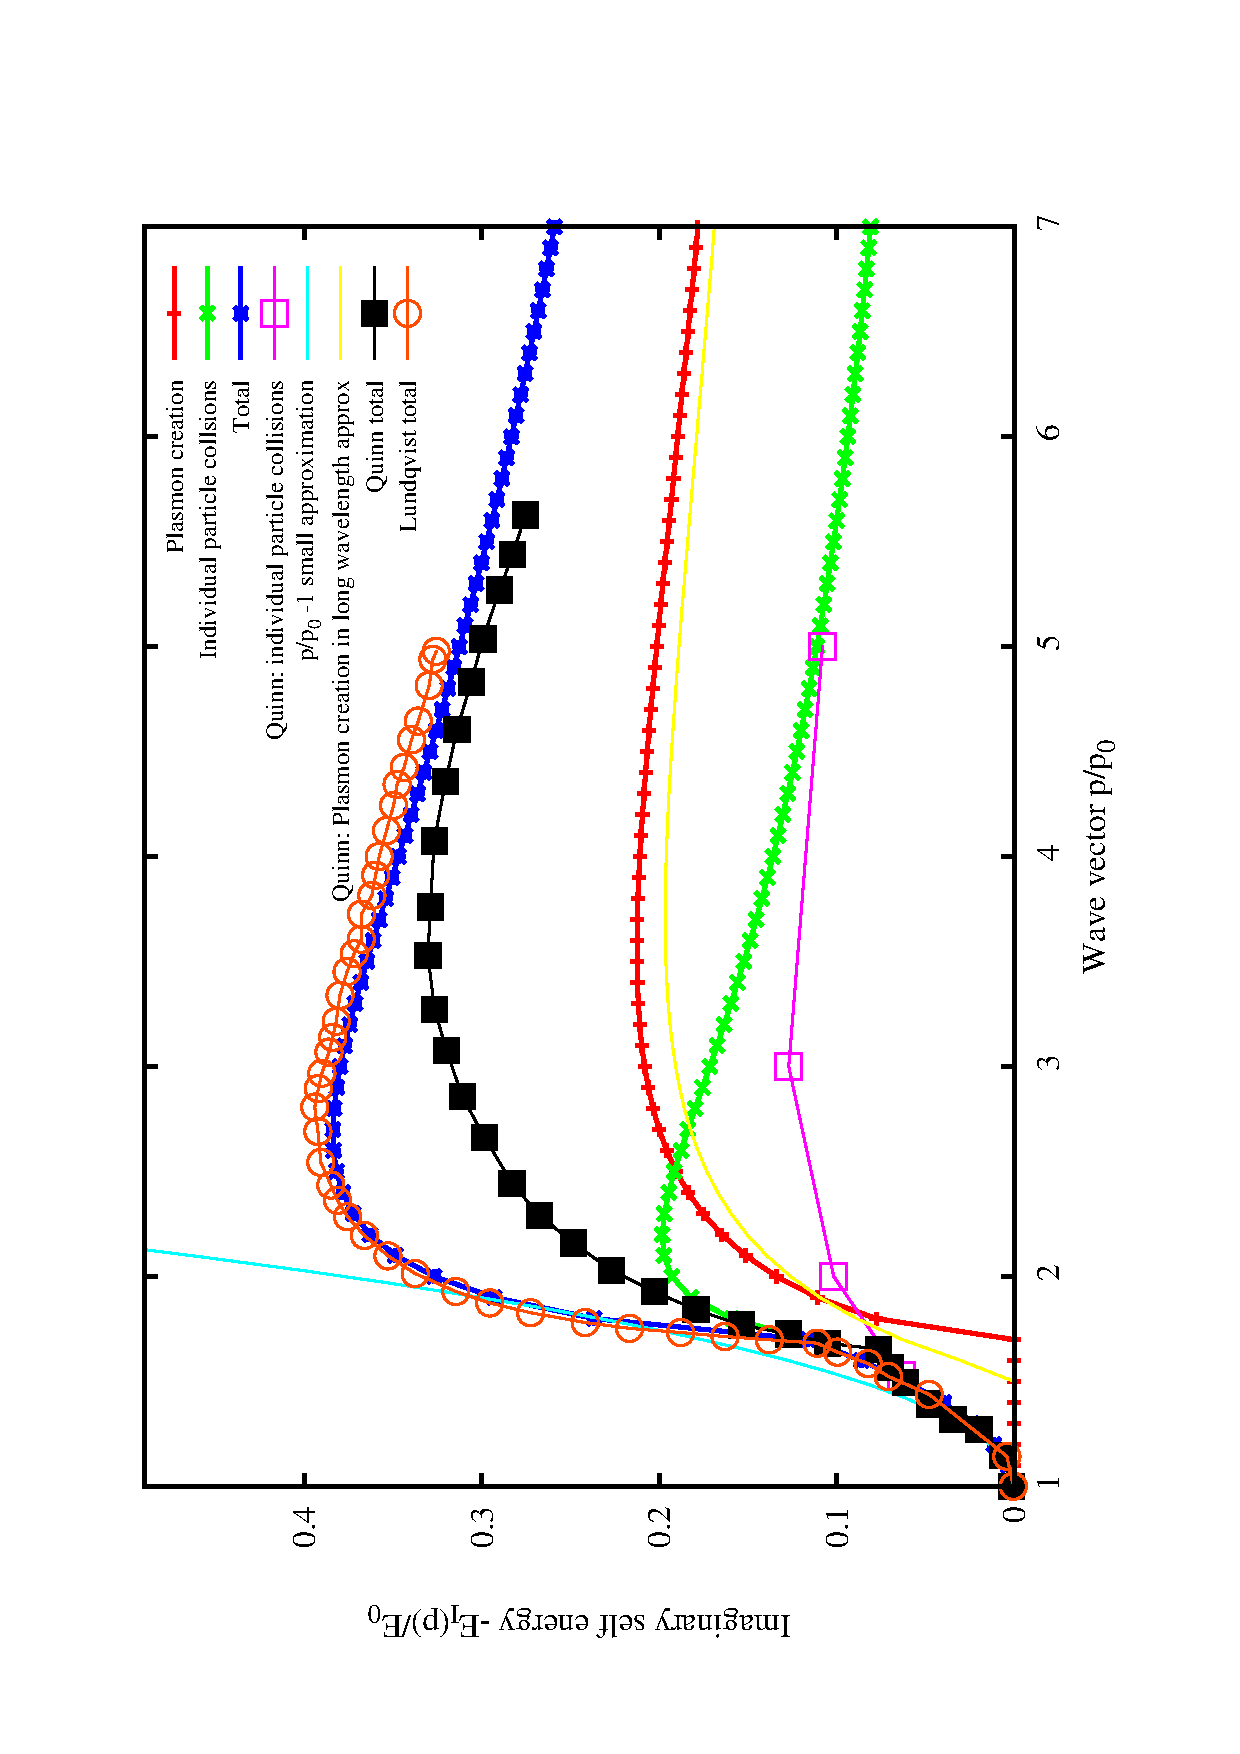
\includegraphics[width=\textwidth]{plots/selfenergyT0-total.pdf}
  \end{center}
  \caption{Total imaginary part of the self-energy for $r_s=2$ at T=0.
  Our calculations - the first three in the legend- are compared to the first calculations by Quinn\cite{Quinn1962},
  and later ones by Lundquist\cite{Lundqvist}.
  The agreement with the later calculations is very good.
  }
  %path: ~/homework/Landaudamping/QM/degenerate/selfenergy/oldimplementaion/selfenergy.ps
  \label{fig:selfenergyT0-total}
\end{figure}
%%%%%%%%%%%%%%%%%%%%%%%%%%%%%%%%%%%%%%%%%%%%%%%%%%%%%%%%%%%%%%%%%%%%%%%%%%%%%%%% 
\subsection{Quasiparticle lifetimes for $T>0$ }
\begin{itemize}
  \item rough description of approximation
  \item results for full calc for several temperatures
  \item calcs for kbT=Ef with
    \begin{itemize}
      \item T=0 distribution function + $T>0$ eps
  	\item picture of integration domain + integrand  for this case, because
	  it is easy to show
      \item $T>0$ distribution function + T=0 eps
      \item picture of distribution function in some meaningful way
	(blurring around Pauli blocking line for set K and T in previous plot. Preferably for K=1.8 , where there is significant change in Im(1/eps))
    \end{itemize}
\end{itemize}
\subsubsection{Procedure}

%%%%%%%%%%%%%%%%%%%%%%%%%%%%%%%%%%%%%%%%%%%%%%%%%%%%%%%%%%%%%%%%%%%%%%%%%%%%%%%% 
%%%%%%%%%%%%%%%%%%%%%%%%%%%%%%%%%%%%%%%%%%%%%%%%%%%%%%%%%%%%%%%%%%%%%%%%%%%%%%%% 
\clearpage
\section{Semiclassical transport}
%\subsection{Effective momentum relaxation rate}
\begin{itemize}
  \item Boltzmann equation in the weak field case\\
    iteration formula see old writeup, Ridley's book 
  \item longwavelength limit - constant plasma frequency
   formally identical to LO phonon scattering\\
   ladder method, see Ridley Book, papers by Delves, Fletcher and Butler 
   etc (references therein)\\
   I haven't found one with a great benchmark, possibly the plot in F+B the best.
 \item Martin Vaughan gave me a writeup and a piece of code on this ages ago. 
   It's not straightforwardly generalizable as far as I remember, but if I 
   could understand what's going on in it I'd have a decent benchmark for 
   starting out
 \item Problem: I don't know in how far any of these use the degenerate case, which
   is what I'd naturally start with.
   \end{itemize}

%%%%%%%%%%%%%%%%%%%%%%%
% ~/homework/writeup/
% I kept the same notation to be as compatible as possible.
%%%%%%%%%%%%%%%%%%%%%%
%%%%%%%%%%%%%%%%%%%%%%%%%%%%%%%%%%%%%%%%%%%%%%%%%%%%%%%%%%%%%%%%%%%%%%%%%%%%%%%% 
\subsection{Three-dimensional mobility}
\label{sec:3d-mobility}
%%%%%%%%%%%%%%%%%%%%%%%%%%%%%%%%%%%%%%%%%%%%
In weak field transport, where the perturbation in the distribution function
is proportional to the applied field, the drift velocity is proportional is 
also proportional to the distribution function. 
The proportionality constant between the drift velocity and the applied field is called mobility.

%%%%%%%%%%%%%%%%%%%%%%
\begin{figure}[tb]
 \setlength{\unitlength}{.7cm}
  \begin{center}
  \begin{picture}(10,10)
    \Large
    %angles
    \put(1,2.5){$\theta$}
    %vecors
    \put(0,8){$\vec e_z \parallel$ $\vec \epsilon$}
    \put(6,4.8){$\vec k$}
    \put(7,1){$\vec e_x$}
    \put(0,0){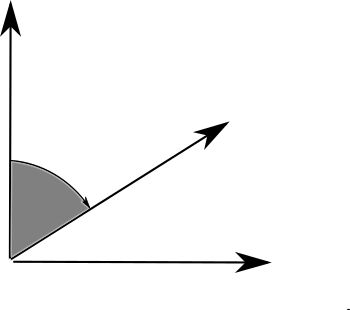
\includegraphics[width = 9\unitlength]{plots/Mobility-angles.pdf}}
  \end{picture}%
  \end{center}
  \caption{Visualisation of important angles for the three-dimensional drift velocity and mobility. 
  We have chosen to depict the x-z plane, but as there is azimuthal symmetry, this picture could be rotated around the z-axis arbitrarily.}
  \label{fig:mobility-angles}
\end{figure}
%%%%%%%%%%%%%%%%%%%%%%
\subsubsection{Drift velocity}
We are only interested in longitudinal transport, i.e., along the field direction.
The drift velocity arises from an average of the group velocity\footnote{citation needed} over the distribution function. 
For parabolic bands, $\vec v(\vec k) =\frac{\hbar}{m}\vec k$.
For the component of the average drift velocity in field direction $\epsilon$,
we find
\begin{equation}
 \left\langle   \vec v_\epsilon \right \rangle
 =\left\langle   \vec v \cdot \vec e_\epsilon \right \rangle
 = \sum\limits_{\vec k} f_{\vec k} \frac{\hbar}{m}\vec k\cdot \vec e_\epsilon.
  \label{eq:v-average}
\end{equation}
Let us use a spherical coordinate system with the z-axis aligned with the 
field direction $\vec e_{\epsilon} =\vec e_z$, so that the angle between $\vec k$
and $\vec \epsilon$ is the polar angle $\theta$.
Let us assume further that our system is isotropic, so that the distribution 
function is independent of the azimuthal angle $\varphi$, see fig.~\ref{fig:mobility-angles}.
We transform the sum into an integral using
$$\sum_{\vec k} = \frac{2}{n(2\pi)^3}\int d^3 \vec k$$
where n is the carrier density.
\begin{equation}
\begin{split}
 \left\langle   \vec v_\epsilon \right \rangle
& = \sum\limits_{\vec k} f_{\vec k} \frac{\hbar}{m} k \cos\theta
 = \frac{2 }{(2\pi)^3} \frac{\hbar}{n m}
 \intd[0][2\pi]\varphi
 \intd[0][\pi]\theta \sin\theta 
 \intd[0][\infty]k k^3 \cos \theta f(k, \theta)\\
& = \frac{2 }{(2\pi)^2} \frac{\hbar}{n m}
 \intd[0][\pi]\theta \sin\theta\cos\theta 
 \intd[0][\infty]k k^3 f(k,\theta)
\end{split}
  \label{eq:v-average2}
\end{equation}
It will prove advantageous shortly to expand the distribution function 
into Legendre polynomials\cite{abramowitzstegun72}:
\begin{equation}
  f(k,\cos\theta) = \sum_{n=0}^\infty f_n(k) P_n(\cos\theta)
  \label{eq:f-legendre}
\end{equation}
%%%%%%%%%%%%%%%%%%%%%%%%%%%%%%%%%%%%%%%%%%%%%%%%%%%%%%%%
\begin{table}
  \centering
  \begin{tabular}{l c  }
   $n$	&	$P_n(x) $ \\\hline
    0	&	1	\\
    1	&	$x$	\\
    2	&	$\frac{1}{2}(3x^2 -1)$	\\	
    3	&	$\frac{1}{2}(5x^3 -3x)$	\\	
  \end{tabular}
  \caption{The four lowest order Legendre polynomials, see~\cite{abramowitzstegun72}}
  \label{tab:legendre-polynomials}
\end{table}
%%%%%%%%%%%%%%%%%%%%%%%%%%%%%%%%%%%%%%%%%%%%%%%%%%%%%%%%
Legendre polynomials obey the orthogonality relation\cite{abramowitzstegun72}
\begin{equation}
  \intd[-1][1]x P_i(x) P_j(x) =\frac{2}{2j+1}\delta_{ij} 
  \text{ or }
  \intd[0][\pi]\theta \sin\theta  P_i(\cos\theta) P_j(\cos\theta) =\frac{2}{2j+1}\delta_{ij} 
  \label{eq:legendre-orthogonal}
\end{equation}
The lowest order Legendre polynomials are listed in table~\ref{tab:legendre-polynomials}.
Taking advantage of $P_1(\cos\theta) =\cos\theta$, we can apply the orthogonality
relation to the drift velocity
\begin{equation}
\begin{split}
 \left\langle   \vec v_\epsilon \right \rangle
& = \frac{2 }{(2\pi)^2} \frac{\hbar}{n m}
 \intd[0][\infty]k k^3
 \sum_{n=0}^\infty
 \intd[0][\pi]\theta \sin\theta 
f_n(k) P_n(\cos\theta) P_1(\cos\theta)\\
& = \frac{2 }{(2\pi)^2} \frac{\hbar}{n m}
 \intd[0][\infty]k k^3
 f_1(k) \frac{2}{3}   
 = \frac{\hbar}{3 \pi^2 n  m}
 \intd[0][\infty]k k^3
 f_1(k) \\
& = \frac{\hbar}{m k_F^3}
 \intd[0][\infty]k k^3
 f_1(k), 
\end{split}
  \label{eq:v-average3}
\end{equation}
where $k_F=\sqrt[3]{3\pi^2 n}$ is the Fermi wave vector.

We showed that the drift velocity only depends on the coefficient $f_1(k)$ of the
distribution function when expanded into Legendre polynomials.

\subsubsection{Mobility}
If this $f_1(k)= a(k) \epsilon$ is proportional to the applied field 
with some proportionality constant $a(k)$, 
the mobility is
\begin{equation}
  \mu =  \frac{\hbar}{m k_F^3}\intd[0][\infty]k k^3 a(k) 
  \label{eq:3d-mobility}
\end{equation}

%%%%%%%%%%%%%%%%%%%%%%%%%%%%%%%%%%%%%%%%%%%%
\subsection{Three-dimensional Boltzmann equation}
This section follows the description in \cite{RID99}.
Let f($\vec x$, $\vec v$, t) be the distribution function of the carriers.
According to the Boltzmann equation for semiclassical transport\footnote{Citation needed?}
\begin{equation}
  \frac{d f}{d t}=\frac{\partial f}{\partial t} +\frac{\partial f}{\partial x_i}\frac{\hbar k_i}{m}+\frac{\partial f}{\partial k_i}\frac{F_i}{\hbar}=\left(\frac{\partial f}{\partial t}\right)^{coll},
  \label{eq:Boltzmann}
\end{equation}
the changes to the distribution function are either due to drift, an external field, or collisions.

In the following, we are looking for a spacially uniform, stationary solution,\begin{equation}
  \frac{d f_{\vec k}}{d t}
  =\frac{\partial f_{\vec k}}{\partial k_i}\frac{F_i}{\hbar}
  =\left(\frac{\partial f_{\vec k}}{\partial t}\right)^{coll},
  \label{eq:Boltzmanneqstationaryuniform}
\end{equation}
so that only the collision and the field term are left, and the distribution function only depends on the wave vector $\vec k$. 

If $P_{\vec k,\vec{k'}}$ is the probability per unit time that an electron with wave vector $\vec k$ is scattered into a state with wave vector $\vec{k'}$,
$f_{\vec{k}}$ is the probability that the electron state with wave vector $\vec k$ is occupied and $1-f_{\vec{k'}}$ that the state with $\vec{k'}$ unoccupied, 
\[
P_{\vec k,\vec{k'}}f_{\vec k}(1-f_{\vec{k'}})
\]
yields the probability of a collision which changes the electron's wave vector from $\vec{k}$ to $\vec{k'}$. Therefore, the change rate of the distribution due to collisions 
\begin{equation}
  \left(\frac{\partial f_{\vec{k}}}{\partial t}\right)^{coll}
  =\sum\limits_{\vec{k}\neq\vec{k'}}
  \left[P_{\vec{ k'},\vec{k}}f_{\vec{k'}}(1-f_{\vec{k}})-P_{\vec k,\vec{k'}}f_{\vec k}(1-f_{\vec{k'}})\right]
  \label{eq:collisionterm}
\end{equation}
is the difference between the number of collisions per unit time that leave an electron in a state with wave vector $\vec k$, and the number of collisions per unit time that scatter an electron from a state with wave vector $\vec{k}$, see, e.g.,~\cite{asc87}.
\subsubsection{Expansion of the Boltzmann equation into Legendre polynomials}
As we saw in section \ref{sec:3d-mobility}, the drift velocity only depends on 
the projection of the distribution function on the $n=1$ Legendre polynomial.
We will therefore expand the stationary Boltzmann equation
\begin{equation}
  \frac{\partial f_{\vec k}}{\partial \vec k} \cdot \frac{\vec F}{\hbar}
  =\sum\limits_{\vec{k}\neq\vec{k'}}
  \left[P_{\vec{ k'},\vec{k}}f_{\vec{k'}}(1-f_{\vec{k}})-P_{\vec k,\vec{k'}}f_{\vec k}(1-f_{\vec{k'}})\right]
  \label{eq:stationary-collisonal-boltzmann}
\end{equation}
%%%%%%%%%%%%%%%%%%%%%%
into Legendre polynomials using eq.~(\ref{eq:f-legendre}).
\subsubsection{Field-free case}
When there is no field present, the left hand side of equation~(\ref{eq:stationary-collisonal-boltzmann}) vanishes. 
Without the disturbance, there is no preferred direction either, and
the distribution function is spherically symmetric.
That is exactly the $f_0(k)$ contribution of the expansion of $f$ into
Legendre polynomials. 
It fulfills the relation
\begin{equation}
  0=\sum\limits_{\vec{k}\neq\vec{k'}}
  \left[P_{\vec{ k'},\vec{k}}
  f_0(k')(1-f_0(k))-
  P_{\vec k,\vec{k'}}
  f_0( k)(1-f_0(k'))\right]
  \label{eq:equilibrium-boltzmann}
\end{equation}
The solution for this is the Fermi-Dirac distribution function.\footnote{H-theorem,etc, citation needed!}

\subsubsection{Weak field approximation}
An expansion of equation~(\ref{eq:stationary-collisonal-boltzmann})
leads to a hierarchy of equations for the coefficients $f_n(k)$,
so that $f_{n-1}$ depends on $f_n$ and so on.
\alert{Give explicitly later?}
As long as the applied field is sufficiently small, we can circumvent this:\\
If the field $\vec F$ is small, so will be the deviation $f(\vec k) -f_0(k)$ in realtion to the field free distribution function $f_0(k)$. 
In the so-called zeroth order of the approximation, the field is vanishingly small, and the the distribution function is the field-free one.

In first order, we plug in the field-free solution for $f_0(k)$ in $f_{\vec k} = f_0(k) + f_1(k) P_1(\cos\theta)$, but only retain first order terms,
before we solve the equation for $f_1(k)$. 
All second order or higher terms, such as the products $F f_1$ or $f_1(k) f_1(k')$, are much smaller than the first order terms and will be neglected.

\paragraph*{Left hand side}
Expressed in spherical coordinates $(k,\theta,\varphi)$, the gradient of a function which is independent of the azimuthal angle is 
\[
  \frac{\partial f_{\vec k}}{\partial \vec k} = 
  \frac{\partial f_{\vec k}}{\partial k} \vec e_k + 
  \frac{1}{k}  \frac{\partial f_{\vec k}}{\partial \theta } \vec e_\theta  
  \text{ with }
  \vec e_k =	\begin{pmatrix}
    			\sin\theta\cos\varphi\\
    			\sin\theta\sin\varphi\\
    			\cos\theta
		\end{pmatrix}
  \text{ and }
  \vec e_\theta =\begin{pmatrix}
    			\cos\theta\cos\varphi\\
    			\cos\theta\sin\varphi\\
    			-\sin\theta
		\end{pmatrix}
\]
As the field $F$ defines the z-direction, we get 
\begin{equation}
  LHS = 
  \frac{F}{\hbar}  \left( \frac{\partial f_{\vec k}}{\partial k} \cos\theta
  -\frac{1}{k}  \frac{\partial f_{\vec k}}{\partial \theta } \sin\theta  \right)
  = \frac{F}{\hbar} \sum_{n=0}^\infty
  \left[
  \frac{\partial f_n(k)}{\partial k} P_n(\cos\theta)\cos\theta
  +\frac{f_n(k)}{k} \frac{\partial P_n(\cos\theta) }{\partial \cos\theta} \sin^2\theta 
  \right]
  \label{eq-Boltzmann-LHS}
\end{equation}
For the first order approximation of this, we only retain the $n=0$ terms in the sum:
\begin{equation}
  LHS_1  
  = \frac{F}{\hbar} 
  \frac{\partial f_0(k)}{\partial k} P_0(\cos\theta)\cos\theta
  +\frac{f_0(k)}{k} \frac{\partial P_0(\cos\theta) }{\partial \cos\theta} \sin^2\theta 
  = \frac{F}{\hbar} 
  \frac{\partial f_0(k)}{\partial k}\cos\theta
  \label{eq-Boltzmann-LHS-1}
\end{equation}
%%%%%%%%%%%%%%%%%%%%%
\paragraph*{Right hand side}
In order to evaluate the right hand side of eq.~(\ref{eq:stationary-collisonal-boltzmann}), we plug in $f_{\vec k} = f_0(k) +f_1(k)P_1(\cos\theta)$, but neglect all 
product terms of order $f_1^2$.
\[
\begin{split}
f_{\vec k'}(1-f_{\vec k}) =
&\left[ f_0(k') +f_1(k')\cos\theta'\right]
\left[1-f_0(k) -f_1(k)\cos\theta\right] +\text{ 2$^{nd}$ order}\\
=&f_0(k') \left[1-f_0(k)\right] \text{ 0$^{th}$ order}\\
-&f_0(k')f_1(k)\cos\theta
+f_1(k')\cos\theta'\left[1-f_0(k)\right] \text{ 1$^{st}$ order}\\
+&\text{ 2$^{nd}$ order}
\end{split}
\]
If we plug in the expression above into the right hand side of the stationary
Boltzmann equation~(\ref{eq:stationary-collisonal-boltzmann}), we see that 
it contains a term which is zero according to the zeroth order Boltzmann
equation~(\ref{eq:equilibrium-boltzmann}). 
The remaining right hand side part is
\begin{equation}
  \begin{split}
  RHS_1  
  =\frac{1}{n(2\pi)^3} \intd{^3\vec k'}  
  \left\{
  	 P_{\vec k',\vec k}
	 \left[ 
		f_1(k')\cos\theta'\left[1-f_0(k)\right]
	 	-f_0(k')f_1(k)\cos\theta
	\right]\;\; 
		\right.\\ \left.
  	-P_{\vec k,\vec k'}
	 \left[
		f_1(k)\cos\theta\left[1-f_0(k')\right]
		-f_0(k)f_1(k')\cos\theta'
	\right] 
  \right\}
  \end{split}
  \label{eq-Boltzmann-RHS-1}
\end{equation}
%%%%%%%%%%%%%%%%%%%%%%%
\paragraph*{Boltzmann equation in first order}
%%%%%%%%%%%%%%%%%%%%%%%
We can now give the Boltzmann equation for the weak field correction in first order.
\begin{equation}
  \begin{split}
\frac{F}{\hbar} 
  \frac{\partial f_0(k)}{\partial k}\cos\theta
  =\frac{1}{n(2\pi)^3} \intd{^3\vec k'}
  \left\{
  	 P_{\vec k',\vec k}
	 \left[ 
		f_1(k')\cos\theta'\left[1-f_0(k)\right]
	 	-f_0(k')f_1(k)\cos\theta
	\right]\;\; 
		\right.\\ \left.
  	-P_{\vec k,\vec k'}
	 \left[
		f_1(k)\cos\theta\left[1-f_0(k')\right]
		-f_0(k)f_1(k')\cos\theta'
	\right] 
  \right\}.
  \end{split}
  \label{eq:Boltzmann-1}
\end{equation}
%%%%%%%%%%%%%%%%%%%%%%%%%%%%%%%%%%%%%%%%%%%%%%%%%%%%%%%%%%%%%%
\subsection{Solution of the Boltzmann equation for weak fields}
%%%%%%%%%%%%%%%%%%%%%%%%%%%%%%%%%%%%%%%%%%%%%%%%%%%%%%%%%%%%%%
If the field is perpendicular to the wave vector direction, the equation vanishes.
Otherwise, we can divide both sides by $\cos\theta$, which yields
\begin{equation}
  \begin{split}
\frac{F}{\hbar} 
  \frac{\partial f_0(k)}{\partial k}
  =\frac{1}{n(2\pi)^3} \intd{^3\vec k'}
  \left\{
  	 P_{\vec k',\vec k}
	 \left[ 
	 f_1(k')\left[1-f_0(k)\right]\frac{\cos\theta'}{\cos\theta}
	 	-f_0(k')f_1(k)
	\right]\;\; 
		\right.\\ \left.
  	-P_{\vec k,\vec k'}
	 \left[
		f_1(k)\left[1-f_0(k')\right]
		-f_0(k)f_1(k')\frac{\cos\theta'}{\cos\theta}
	\right] 
  \right\}.
  \end{split}
  \label{eq:Boltzmann-1b}
\end{equation}
Note that this expression involves two different angles - 
$\theta$ is the polar angle between the field direction $\vec F$ and $\vec k$, 
and $\theta'$ the polar angle between $\vec F$ and $\vec k$.

If we regroup the previous equation a bit, 
\begin{equation}
  \begin{split}
\underbrace{
	\frac{F}{\hbar} 
	\frac{\partial f_0(k)}{\partial k}
	}_{A(k)}
  =  -f_1(k)
\underbrace{
\frac{1}{n(2\pi)^3} \intd{^3\vec k'}
	  \left\{
  		P_{\vec k,\vec k'}
			\left[1-f_0(k')\right]
		 +P_{\vec k',\vec k} 
		 	f_0(k')
	  \right\}
	  }_{B(k)}
  \\+
\underbrace{
\frac{1}{n(2\pi)^3} \intd{^3\vec k'}
	  f_1(k')\frac{\cos\theta'}{\cos\theta}
	\left\{
  		  P_{\vec k',\vec k}
		  	\left[1-f_0(k)\right]
  		+P_{\vec k,\vec k'}
			f_0(k)		\right\}	 
			}_{C(k,\{f_1\})}
  \end{split}
  \label{eq:Boltzmann-1b}
\end{equation}
it becomes more obvious to see that it is an integral equation, where
$f_1(k)$ depends on an integral over $f_1(k)$ itself.
\begin{equation}
  f_1(k) = \frac{1}{B(k)}\left[ C(k, \{f_1\}) -A(k) \right]
  \label{eq:f1-integral}
\end{equation}
Here we have introduce shorthands for the integrals above. 
The notation $C(k,\{f_1\})$ means that $C$ depends on k, and the function $f_1(k)$.
%%%%%%%%%%%%%%%%%%%%%%%%%%%%%%%%%%%%%%%%%%%%
\subsubsection{Elastic scattering}
%%%%%%%%%%%%%%%%%%%%%%%%%%%%%%%%%%%%%%%%%%%%
If the scattering processes are elastic, i.e., $k = k'$, the first order Boltzmann 
equation becomes significantly easier.
Due to the equilibrium condition eq.~(\ref{eq:equilibrium-boltzmann}), we find 
$P_{\vec k',\vec k} = P(k,\theta; k',\theta') = P(k,\theta; k,\theta')$ and hence
\begin{equation}
	\frac{F}{\hbar} 
	\frac{\partial f_0(k)}{\partial k}
  =  f_1(k)
  \frac{1}{n(2\pi)^3} \intd{^3\vec k'}  
	 \left[ \frac{\cos\theta'}{\cos\theta}-1\right]
  		  %P_{\vec k',\vec k},
  		  P(k,\theta; k,\theta'),
  \label{eq:Boltzmann-1-elastic}
\end{equation}
so that we can solve for $f_1(k)$
\begin{equation}
f_1(k)=\frac{
	\frac{F}{\hbar} \frac{\partial f_0(k)}{\partial k}
  	}{
	\underbrace{
	\frac{1}{n(2\pi)^3} \intd{^3\vec k'}
	 \left[ \frac{\cos\theta'}{\cos\theta}-1\right]
  		  %P_{\vec k',\vec k}
		  P(k,\theta; k,\theta')
		  }_{E(k)}
	 }
  \label{eq:Boltzmann-1-elastic}
\end{equation}
With eq.~(\ref{eq:cosalphaKW}) in the limit $\frac{W}{K^2}\ll 1$, 
we have 
\begin{equation}
  \cos\alpha^{\stackrel{em}{ab}}
    =\frac{K}{\sqrt{K^2\mp W}}\left(1-\frac{Q^2\pm W}{2K^2}\right)
    \stackrel{\frac{W}{K^2}\to0}{\longrightarrow} \left(1-\frac{Q^2}{2K^2}\right),
  \label{eq:cosalphaKW-elastic}
\end{equation}
so that $\frac{\cos\theta'}{\cos\theta}-1 \stackrel{\frac{W}{K^2}\to0}{\longrightarrow}-\frac{Q^2}{2K^2}$.

We will plug this expression back into $E(k)$, noting, however, that the integration only makes sense in the case where $K^2\ll W$.  
We will identify the elastic regime by comparing the approximately elastic 
solution to the full solution of the inelastic equations.
\begin{equation}
  \begin{split}
    E(K) =
  - \frac{2E_F}{n\hbar \pi a_0k_F K^3} 
 & \left\{
\intd[0][2K]{Q}Q
  \int\limits_{0}^{Q\left(2K-Q\right)}\!\!\!\!\!\!\mathrm{d}W\,
\mathfrak{Im}\left(\frac{1}{\varepsilon(W,Q)}\right) 
\right.\\
&\left. + \intd[0][2K]{Q}Q
  \int\limits_{0}^{Q\left(2K+Q\right)}\!\!\!\!\!\!\mathrm{d}W\,
\mathfrak{Im}\left(\frac{1}{\varepsilon(W,Q)}\right) 
+ \intd[0][2K]{Q}Q
  \int\limits_{Q\left(Q-2K\right)}^{Q\left(Q+2K\right)}\!\!\!\!\!\!\mathrm{d}W
\mathfrak{Im}\left(\frac{1}{\varepsilon(W,Q)}\right) 
\right\}
  \label{eq:EK}
\end{split}
\end{equation}
%%%%%%%%%%%%%%%%%%%%%%%%%%%%%%%%%%%%
\alert{Do I need to mention the relaxation time approximation?}
\alert{I don't quite know where best to put this. Maybe further down}
\alert{REORGANISE THIS SECTION!}
%%%%%%%%%%%%%%%%%%%%%%%%%%%%%%%%%%%%%%%%%%%%%%%%%%%%%%%%%%%%%%%%%%%%%%%%%%%%%%%
\subsubsection{Iterative solution for inelastic scattering}
%%%%%%%%%%%%%%%%%%%%%%%%%%%%%%%%%%%%%%%%%%%%%%%%%%%%%%%%%%%%%%%%%%%%%%%%%%%%%%%
For inelastic scattering, however, we cannot solve eq.~(\ref{eq:f1-integral}) for $f_1(k)$ analytically, because it depends on itself at different wave vectors.
Equation ~(\ref{eq:f1-integral}) has been solved iteratively for certain cases, however.
In longitudinal optical (LO) phonon scattering, the transferred energy $\hbar \omega$ is independent of the transferred wave vector, so that $f_1(k)=\tilde{f}_1(E(k))$ is only linked to $\tilde{f}_1(E(k) + n\hbar \omega)$, and a solution can be found more easily,\cite{Delves1959,Fletcher-Butcher}.
%%%%%%%%%%%%%%%%%%%%%%
\paragraph*{Procedure}
%%%%%%%%%%%%%%%%%%%%%%
We start at an initial guess for $y_0(k)$.
Then we plug in the initial guess in the right hand side of eq.~(\ref{eq:f1-integral}), and take the left hand side as our next solution.
\begin{equation}
  y_{n+1}(k) = \frac{1}{B(k)}\left[ C(k, \{y_n\}) -A(k) \right]
  \label{eq:f1-iteration}
\end{equation}
If, for some large $n_1, n_2$, the difference between $y_{n1}(k)$ and $y_{n2}(k)$ becomes arbitrarilyly small, we consider the solution as converged, 
and $\lim_{n\to\infty}y_n =f_1(k)\approx y_{n1}$.
\alert{This was a very lalala explanation of the Cauchy criterion for 
sequences. It would be nice if I could deliver a requirement on the A, B and C for convergence.} 

The final solution, as well as any intermediate function $y_n$, needs to be much
smaller than $f_0$ for each k, otherwise the iteration formula 
does not hold in the first place.
%%%%%%%%%%%%%%%%%%%%%%
\paragraph*{Detailed expressions}
Let us have a look at the exact expressions the iteration will involve.
We can simplify $B$ and $C$ by eliminating one of the 
scattering rates, if we use eq.~(\ref{eq:equilibrium-boltzmann}): 
\begin{equation}
  \begin{split}
&  B(k)\stackrel{f_0(k)\neq 1}{=}
\frac{1}{n(2\pi)^3} \intd{^3\vec k'}  
  		P_{\vec k,\vec k'}
			\frac{1-f_0(k')}{1-f_0(k)}
			\text{ or }\\
&  B(k)\stackrel{f_0(k)\neq 0}{=}
\frac{1}{n(2\pi)^3} \intd{^3\vec k'  }
  		P_{\vec k',\vec k}
			\frac{f_0(k')}{f_0(k)}
  \end{split}
  \label{eq:Bk}
\end{equation}
The division by the distribution functions is only a concern for very small or very large wave vectors, or at very low temperatures. We will discuss this case individually later.

Similarily, we can modily $C$, so that
\begin{equation}
  \begin{split}
    &C(k,\{f_{1}\}) \stackrel{f_0(k')\neq 0}{=}
f_0(k)\frac{1}{n(2\pi)^3} \intd{^3\vec k'  }
	\frac{f_1(k')}{f_0(k')} \frac{\cos\theta'}{\cos\theta}
  		  P_{\vec k,\vec k'}
\text{ or }\\
&C(k\{f_{1}\}) \stackrel{f_0(k')\neq 1}{=}
\left[1-f_0(k)\right]\frac{1}{n(2\pi)^3} \intd{^3\vec k'  }
	\frac{f_1(k')}{1-f_0(k')} \frac{\cos\theta'}{\cos\theta}
  		  P_{\vec k',\vec k}
  \end{split}
  \label{eq:Ck}
\end{equation}
The integrals over $k'$ will be singular for $k'\to0$ and $k'\to\infty$ 
unless the rest of the integrand -including $f_1(k)$ goes to zero faster than $f_0(k)$ in those limits.
\alert{With that said though, I'm not sure if this way of writing it is helpful, or if I'm just bringing thouse singularities upon myself by eliminating Pkk' or Pk'k.
}

\alert{Edit: As far as I understand it, there is no difference between Ridley's effective
relaxation time approach and this, except that Ridley divides by f0, f0', 1-f0, 1-f0' an awful lot. Might be worth going through with this, especially for the T=0 case}
%%%%%%%%%%%%%%%%%%%%%%
%%%%%%%%%%%%%%%%%%%%%%%%%%%%%%%%%%%%%%%%%%
\paragraph*{Fermi Golden Rule}
%%%%%%%%%%%%%%%%%%%%%%%%%%%%%%%%%%%%%%%%%%
It follows from Fermi's Golden Rule\cite{Dirac-fermi-golden-rule1927}
that the scattering rate 
$  P_{\vec k, \vec k'}$ includes a delta function which makes sure that 
energy is conserved.
\begin{equation}
  P_{\vec k, \vec k'}= 
  \frac{2\pi}{\hbar} 
  \intd[-\infty][\infty]{\hbar\omega}|M_{\omega,\vec k,\vec k'}|^2 \delta\left(E' - E +\hbar\omega \right)
  \label{eq:FermiGoldenRule-variation}
\end{equation}
Here, $\hbar\omega$ is the transferred energy, and $M$ is the scattering matrix element.
It can be instructive to seperate processes where energy is emitted $E>E'$, 
and processes where energy is absorbed $E<E'$.
\begin{equation}
  P_{\vec k, \vec k'}= 
  \underbrace{
  \frac{2\pi}{\hbar} 
 \intd[0][\infty]{\hbar\omega }|M_{-\omega,\vec k,\vec k'}|^2 \delta\left(E' - E -\hbar\omega \right)
  }_{Absorption}
+ 
  \underbrace{
  \frac{2\pi}{\hbar} 
\intd[0][\infty]{\hbar\omega} |M_{\omega,\vec k,\vec k'}|^2 \delta\left(E' - E +\hbar\omega \right)
  }_{Emission}
  \label{eq:FermiGoldenRule-variation-em-ab}
\end{equation}
If we assume that the scattering rate $M_{\omega,\vec k, \vec k'}$ only depends on the 
transferred wave vector $\vec q = \vec k -\vec k'$, and not on $\vec k$ and $\vec k'$
individually, 
\begin{equation}
  M_{\omega,\vec k,\vec k'} = M_{\omega,\vec q},
  \label{eq:Matrix-element-q}
\end{equation}
it is useful to transform the integrals over $\vec k'$ above into
integrals over $\vec q$.

According to Fermi's Golden rule, the scattering rate $P_{\vec k}$ is the integral of $P_{\vec k,\vec k'}$ 
times the density of final states 
over the final state (wave vectors) $\vec k'$.
In first order, this is
\begin{equation}
  P_{\vec k} =\sum_{\vec k'} P_{\vec k,\vec k'} (1-f_0(k'))
  \label{eq:Scattering-rate}
\end{equation}
and the final wave vector $\vec k'$ is
\begin{equation}
  \vec k' =|\vec k -\vec q| = \sqrt{k^2 +q^2 -2 kq \cos\theta_q},
  \label{eq:kprime}
\end{equation}
where $\theta_q$ is the angle between $\vec q$ and $\vec k$.
%%%%%%%%%%%%%%%%%%%%%%
\paragraph*{Emission}
Hence, 
\begin{equation}
  P^{em}_{\vec k} =\frac{1}{n(2\pi)^3}\intd{^3\vec q} 
  %P^{em}_{\vec k,\vec k'}
  \frac{2\pi}{\hbar} 
  \intd[-\infty][\infty]{\hbar\omega}  |M_{\omega,\vec q}|^2 \delta\left(E' - E +\hbar\omega \right)
  (1-f_0( \sqrt{k^2 +q^2 -2 kq \cos\theta_q})),
  \label{eq:Scattering-rate2}
\end{equation}
where the integratin over $\vec k'$ has been replaced by one over $\vec q$.
The integration is carried out in spherical coordinates. 
Assuming $M_{\vec q}$ is independent of $\varphi_q$, the integral over the azimuthal angle $\varphi_q$ can be carried out immediately and yields $2\pi$.
We will keep the integral over frequency, and use the delta function to carry out the integral over  $\cos\theta_q=u$.
That is the same as setting
\begin{equation}
  \cos\theta_q=\frac{q^2 +\frac{2m}{\hbar}\omega}{2kq}
  \label{eq:costhetaq-em}
\end{equation}
everywhere.
\begin{equation}
  \begin{split}
  P^{em}_{\vec k} &
  = \frac{1}{ 2\pi n \hbar}\intd[0][\infty]q q^2\intd[-1][1]u
  \intd[0][\infty]{\hbar\omega}|M_{\omega,q,u}|^2
  (1-f_0( \sqrt{k^2 +q^2 -2 kq u}))
  \delta\left(\frac{\hbar^2}{2m}\left(q^2  - 2kq u \right) +\hbar\omega \right)\\
 & =\frac{1}{ 2\pi n \hbar}
  \frac{m}{\hbar^2 k}
 \intd[0][\infty]q q
 \intd[0][\infty]{\hbar\omega}
  |M_{\omega,q, \frac{q^2 +2m\omega/\hbar}{2kq}}|^2
(1-f_0( \sqrt{k^2 -\frac{2m}{\hbar}\omega})) 
\text{ if } -1\leq\frac{q^2 +2m\omega/\hbar}{2kq}\leq 1
  \label{eq:Scattering-rate3}
  \end{split}
\end{equation}
We see that the energy conservation moved from the argument of the delta-function
to the limits of the two-dimensional integral over transferred energy and wave vector.
If the integral over wave vector is carried out first, 
$\frac{q^2 +2m\omega/\hbar}{2kq}\leq 1$
can be expressed as
$\hbar\omega\leq \frac{\hbar^2}{2m}\left(2kq-q^2\right)$. 
In order for $\omega$ to be positive, we furthermore need $q\leq2k$.
This yields
\begin{equation}
  P^{em}_{\vec k} 
  =\frac{1}{ 2\pi n \hbar}
  \frac{m}{\hbar^2 k}
  \intd[0][2k]q q
  \intd[0][\frac{\hbar^2}{2m}\left(2kq-q^2\right)]{\hbar\omega}
  |M_{\omega,q, \frac{q^2 +2m\omega/\hbar}{2kq}}|^2
(1-f_0( \sqrt{k^2 -\frac{2m}{\hbar}\omega})) 
  \label{eq:Scattering-rate4}
\end{equation}
%%%%%%%%%%%%%%%%%%%%%%
\paragraph*{Absorption}
Similarly, if we consider absorption, using
\begin{equation}
  \cos\theta_q=\frac{q^2 -\frac{2m}{\hbar}\omega}{2kq}
  \label{eq:costhetaq-ab}
\end{equation}
we find
\begin{equation}
  \begin{split}
  P^{ab}_{\vec k}
&  =\frac{1}{n(2\pi)^3}\intd{^3\vec q} 
  \frac{2\pi}{\hbar} 
  \intd[0][\infty]{\hbar\omega}|M_{-\omega,\vec q}|^2 \delta\left(E' - E -\hbar\omega \right)
  (1-f_0( \sqrt{k^2 +q^2 -2 kq \cos\theta_q}))\\
& = \frac{1}{ 2\pi n \hbar}\intd[0][\infty]q q^2\intd[-1][1]u
 \intd[0][\infty]{\hbar\omega}|M_{-\omega,q,u}|^2
  (1-f_0( \sqrt{k^2 +q^2 -2 kq u}))
  \delta\left(\frac{\hbar^2}{2m}\left(q^2  - 2kq u \right) -\hbar\omega \right)\\
 & =\frac{1}{ 2\pi n \hbar}
  \frac{m}{\hbar^2 k}
 \intd[0][\infty]q q
 \intd[0][\infty]{\hbar\omega}
  |M_{-\omega,q, \frac{q^2 -2m\omega/\hbar}{2kq}}|^2
(1-f_0( \sqrt{k^2 +\frac{2m}{\hbar}\omega})) 
\text{ if } -1\leq\frac{q^2 -2m\omega/\hbar}{2kq}\leq 1
  \end{split}
  \label{eq:Scattering-rate2-ab}
\end{equation}
The left hand side of the inequality in the last line of eq.~(\ref{eq:Scattering-rate2-ab}) is equivalent to
\[
\hbar\omega\leq \frac{\hbar^2}{2m}q(q+2k),
\]
the right hand side to
\[
\hbar\omega\geq \frac{\hbar^2}{2m}q(q-2k).
\]
As the frequency $\omega$ has to be positive, we can split the integral
into two parts and write
\begin{equation}
  \begin{split}
  P^{ab}_{\vec k} 
  =\frac{1}{ 2\pi n \hbar}
  \frac{m}{\hbar^2 k}
&  \left\{
  \intd[0][2k]q q
 \intd[0][\frac{\hbar^2}{2m}q\left(q+2k\right)]
  |M_{-\omega,q, \frac{q^2 -2m\omega/\hbar}{2kq}}|^2
(1-f_0( \sqrt{k^2 +\frac{2m}{\hbar}\omega})) 
\right.\\
&\left.
+  \intd[2k][\infty]q q
  \intd[\frac{\hbar^2}{2m}q\left(q-2k\right)][\frac{\hbar^2}{2m}q\left(q+2k\right)]
  |M_{-\omega,q, \frac{q^2 -2m\omega/\hbar}{2kq}}|^2
(1-f_0( \sqrt{k^2 +\frac{2m}{\hbar}\omega})) 
\right\}
  \end{split}
  \label{eq:Scattering-rate3-ab}
\end{equation}

%%%%%%%%%%%%%%%%%%%%%%%%%%%%%%%%%%%%%%%%%%%%
\paragraph*{Electron-electron scattering in RPA}
\alert{I really have no clue if I can do this. I think I can't, because 
I'm neglecting half of the cases, but this is maybe worth a closer look.}
For electron-electron scattering in the RPA, we use an effective matrix element
\begin{equation}
  M_{eff}^2(\omega,q) = |\frac{4\pi^2 e^2}{q^2 \varepsilon(\omega,q)}|^2
  \frac{q^2}{4\pi^2 e^2}\mathfrak{Im}(\varepsilon(\omega,q))
  =-\frac{4e^2 }{q^2}\mathfrak{Im}(\frac{1}{\varepsilon(\omega,q)}), 
  \label{eq:M_eff}
\end{equation}
see eq.~(\ref{eq:Wk-iminveps}).
With this matrix element, we find
\begin{equation}
  P^{em}_{\vec k}n 
  =-\frac{2}{\hbar}
  \frac{1}{\pi a_0k}
  \int\limits_0^{2k}\frac{\mathrm{d}q}{ q}
  \int\limits_{0}^{\frac{\hbar^2}{2m}q\left(2k-q\right)}\!\!\!\!\!\!\mathrm{d}\hbar\omega\,
\mathfrak{Im}\left(\frac{1}{\varepsilon(\omega,q)}\right) 
\left[1-f_0\left( \sqrt{k^2 -\frac{2m}{\hbar}\omega}\right)\right] 
  \label{eq:Scattering-rate4}
\end{equation}
  already calculated in eq.~(\ref{eq:Wk-kw}).
The scattering rate in absorption is
\begin{equation}
  \begin{split}
  P^{ab}_{\vec k}n 
  =-\frac{2}{\hbar}
  \frac{1}{\pi a_0k}
&  \left\{
\int\limits_0^{2k} \frac{\mathrm{d}q}{ q}
  \int\limits_{0}^{\frac{\hbar^2}{2m}q\left(2k+q\right)}\!\!\!\!\!\!\mathrm{d}\hbar\omega\,
\mathfrak{Im}\left(\frac{1}{\varepsilon(\omega,q)}\right) 
\left[1-f_0\left( \sqrt{k^2 +\frac{2m}{\hbar}\omega}\right)\right] 
\right.\\
&\left. +\int\limits_{2k}^\infty \frac{\mathrm{d}q}{ q}
  \int\limits_{\frac{\hbar^2}{2m}q\left(q-2k\right)}^{\frac{\hbar^2}{2m}q\left(q+2k\right)}\!\!\!\!\!\!\mathrm{d}\hbar\omega 
\mathfrak{Im}\left(\frac{1}{\varepsilon(\omega,q)}\right) 
\left[1-f_0\left( \sqrt{k^2 +\frac{2m}{\hbar}\omega}\right)\right] 
\right\}
  \end{split}
  \label{eq:Scattering-rate4}
\end{equation}
  \alert{Replace this section when you're doing the whole thing properly!}

%%%%%%%%%%%%%%%%%%%%%%%%%%%%
\subparagraph*{Term $B(k)$}
%%%%%%%%%%%%%%%%%%%%%%%%%%%%
This gives us an explicit expression for $B(k)=\frac{P_{\vec k}}{1-f_0(k)}$ 
for when the denominator is nonzero.
When using dimensionless frequencies and wave vectors $W$ and $K$, see above, 
by scaling them with the Fermi energy and wave vector, we find
\begin{equation}
  \begin{split}
    B(K) \stackrel{f_0(K)\neq 1}{=}
&  -\frac{1}{1-f_0(K)}
    \frac{2E_F}{n\hbar \pi a_0k_F K} \times\\
&  \left\{
\int\limits_0^{2K} \frac{\mathrm{d}Q}{Q}
  \int\limits_{0}^{Q\left(2K-Q\right)}\!\!\!\!\!\!\mathrm{d}W\,
\mathfrak{Im}\left(\frac{1}{\varepsilon(W,Q)}\right) 
\left[1-f_0\left(\sqrt{K^2-W}\right)\right] 
\right.\\
&\left. +\int\limits_0^{2K} \frac{\mathrm{d}Q}{Q}
  \int\limits_{0}^{Q\left(2K+Q\right)}\!\!\!\!\!\!\mathrm{d}W\,
\mathfrak{Im}\left(\frac{1}{\varepsilon(W,Q)}\right) 
\left[1-f_0\left(\sqrt{K^2 +W}\right)\right] 
\right.\\
&\left. +\int\limits_{2K}^\infty \frac{\mathrm{d}Q}{Q}
  \int\limits_{Q\left(Q-2K\right)}^{Q\left(Q+2K\right)}\!\!\!\!\!\!\mathrm{d}W
\mathfrak{Im}\left(\frac{1}{\varepsilon(W,Q)}\right) 
\left[1-f_0\left( \sqrt{K^2 +W}\right)\right] 
\right\}
  \label{eq:BK}
\end{split}
\end{equation}
%%%%%%%%%%%%%%%%%%%%%%%%%%%%%%%%%%%%
\subparagraph*{Term $C(k,\{f_1\})$}
%%%%%%%%%%%%%%%%%%%%%%%%%%%%%%%%%%%%
In order to calculate the term $C(k,\{f_1\})$ analoguously to $B(k)$,  we need to express the quotient
$\frac{\cos\theta'}{\cos\theta}$
in terms of the variables $k, q, \varphi_q$ and $\theta_q$.
This can be done by expression $\cos\theta'$ in terms of the angle between 
$\vec k$ and $\vec k'$, say $\alpha$.
It is convenient to align the coordiate system so that $\vec k$ is 
parallel to the $z$-axis, and $\vec k$ and the field direction $\vec \epsilon$
span the $x-z$ plane.
This is illustrated in figure~\ref{fig:Boltzmann-angles}.
%%%%%%%%%%%%%%%%%%%%%%%%%%%%%%%%%%%%%%%%%%%%
\begin{figure}[tb]
 \setlength{\unitlength}{.7cm}
  \begin{center}
  \begin{picture}(10,10)
    \Large
    %angles
    \put(1,2.5){$\theta$}
    \put(1.5,3.5){$\alpha$}
    \put(3,1.7){$\phi$}
    %vecors
    \put(0,8){$\vec e_z \parallel$ $\vec k$}
    \put(6,4.8){$\vec \epsilon$}
    \put(4.8,6){$\vec k'$}
    \put(7,1){$\vec e_x$}
    \put(0,0){\includegraphics[width = 9\unitlength]{plots/Boltzmann-angles.pdf}}
  \end{picture}%
  \end{center}
  \caption{Visualisation of important angles in the three-dimensional Boltzmann transport equation. The angle $\theta'$ between the vectors $\vec k'$ and $\vec \epsilon$ is left out to facilitate a better overview.}
  \label{fig:Boltzmann-angles}
\end{figure}
%%%%%%%%%%%%%%%%%%%%%%%%%%%%%%%%%%%%%%%%%%%%
We see that
\begin{equation}
  \cos\theta'=\vec{e}_{k'}\cdot \vec{e}_\epsilon=
  \begin{pmatrix}
    \sin\alpha\cos\varphi\\
    \sin\alpha\sin\varphi\\
    \cos\alpha
  \end{pmatrix}\cdot%
  \begin{pmatrix}
    \sin\theta\\
    0\\
    \cos\theta
  \end{pmatrix}.
  \label{eq:costhetaprime}
\end{equation}
Carrying out the integration over $\varphi=\varphi_q$, 
\begin{equation}
  \average{\cos\theta'}{\varphi_q}=\frac{1}{2\pi}\intd[0][2\pi]{\varphi_q}
  \left(\cos\theta\cos\alpha +\sin\theta\sin\alpha\sin\varphi_q\right)
  =\cos\theta\cos\alpha,
  \label{eq:costhetaprime-av}
\end{equation}
means averaging out the $\sin\varphi_q$ part of $\cos\theta$.
Now, $\cos\alpha$ can be expressed as
\begin{equation}
  \cos\alpha=\frac{\vec k\cdot \vec k'}{kk'}=\frac{k-q\cos\theta_q}{\sqrt{k^2+q^2-2kq\cos\theta_q}}.
  \label{eq:cosalpha}
\end{equation}
Before we plug this in eq.~(\ref{eq:Ck}), we will find the form it takes after eliminating $\cos\theta_q$ using the different energy-momentum 
conservation relations for emission or absorption.
With equations~(\ref{eq:costhetaq-em}) and~(\ref{eq:costhetaq-ab}), this yields
\begin{equation}
  \cos\alpha^{\stackrel{em}{ab}}
    =\frac{K-\frac{Q^2\pm W}{2K}}{\sqrt{K^2\mp W}}
    =\frac{2K^2-Q^2\mp W}{2K\sqrt{K^2\mp W}}
    =\frac{K}{\sqrt{K^2\mp W}}\left(1-\frac{Q^2\pm W}{2K^2}\right)
  \label{eq:cosalphaKW}
\end{equation}
and we get 
\begin{equation}
  \begin{split}
  C(K,\{f_1\})=
&  -f_0(K)
    \frac{2E_F}{n\hbar \pi a_0k_F K} \times\\
&  \left\{
\int\limits_0^{2K} \frac{\mathrm{d}Q}{Q}
  \int\limits_{0}^{Q\left(2K-Q\right)}\!\!\!\!\!\!\mathrm{d}W\,
\mathfrak{Im}\left(\frac{1}{\varepsilon(W,Q)}\right) 
\frac{f_1\left(\sqrt{K^2-W}\right)}{f_0\left(\sqrt{K^2-W}\right)} 
\frac{K-\frac{Q^2+W}{2K}}{\sqrt{K^2-W}}
\right.\\
&\left. +\int\limits_0^{2K} \frac{\mathrm{d}Q}{Q}
  \int\limits_{0}^{Q\left(2K+Q\right)}\!\!\!\!\!\!\mathrm{d}W\,
\mathfrak{Im}\left(\frac{1}{\varepsilon(W,Q)}\right) 
\frac{f_1\left(\sqrt{K^2+W}\right)}{f_0\left(\sqrt{K^2+W}\right)} 
\frac{K-\frac{Q^2-W}{2K}}{\sqrt{K^2+W}}
\right.\\
&\left. +\int\limits_{2K}^\infty \frac{\mathrm{d}Q}{Q}
  \int\limits_{Q\left(Q-2K\right)}^{Q\left(Q+2K\right)}\!\!\!\!\!\!\mathrm{d}W
\mathfrak{Im}\left(\frac{1}{\varepsilon(W,Q)}\right) 
\frac{f_1\left(\sqrt{K^2+W}\right)}{f_0\left(\sqrt{K^2+W}\right)} 
\frac{K-\frac{Q^2-W}{2K}}{\sqrt{K^2+W}}
\right\},
\end{split}
  \label{eq:CK}
\end{equation}
quite a formidable expression.
The first integrand has a singularity where $W=K^2$, which is when the
wave vector after the scattering event, $K'$ vanishes.
This is at the limit of the integration for $Q=K$.
We see 
\begin{equation}
  \lim\limits_{K'\to0} \cos\alpha^{em}
  =\lim\limits_{W\to K^2} \frac{1}{2K}\sqrt{K^2-W}=0
  \label{eq:cosalphaKprimezero}
\end{equation}
that the first integral vanishes at the edge of its integration regime.

To avoid singularities, $f_0(K')$ needs to be nonzero. 
For finite temperatures, the Fermi-Dirac distribution function 
only becomes zero for very large wave vectors.

The function $f_1$ needs to be such that the singularities 
in the third integral are integrable, that is, vanish faster for large 
wave vectors than $f_0$.

For the $T=0$ case, $f_0 =0$  for all wave vectors larger than the Fermi
wave vector. Thus, it is not a good idea to divide by any distribution 
function, and the case should be considered individually.
\alert{Say this at the beginning}.
%%%%%%%%%%%%%%%%%%%%%%%%%%%%%%%%%%%%
\subparagraph*{Term $A(k)$}
%%%%%%%%%%%%%%%%%%%%%%%%%%%%%%%%%%%%
Finally the term $A(k)=\frac{F}{\hbar}\frac{\partial f_0(k)}{\partial k}$
becomes
\begin{equation}
  A(k)=-F\beta v(k) f_0(k)\left[1-f_0(k)\right]
  \text{ with } v(k) = \frac{\hbar k}{m}
  \label{eq:Ak}
\end{equation}
when we plug in the Fermi-Dirac distribution function explicitly.
Expressed with dimensionless wave vectors, this is
\begin{equation}
  A(K)=-F\beta v_F K f_0(K)\left[1-f_0(K)\right]
  \text{ with the Fermi velocity } v_F = \frac{\hbar k_F}{m}.
  \label{eq:AK}
\end{equation}
%%%%%%%%%%%%%%%%%%%%%%%%%%%%%%%%%%%%
\paragraph*{Relaxation time notation}
%%%%%%%%%%%%%%%%%%%%%%%%%%%%%%%%%%%%
If $A(K)$ is nonzero, i.e., $f_0(K)\neq 1$ and $f_0(K)\neq 1$, we can 
divide equation~(\ref{eq:f1-integral}) by $A(K)$. 
\begin{equation}
  y(K)= \frac{1}{B(K)}\left[ C(K,\{y\}) -A(K)\right]
  \stackrel{A(K)\neq 0}{\Leftrightarrow}
  \frac{y(K)}{A(K)}= \frac{1}{B(K)}\left[ \frac{C(K,\{y\})}{A(K)} -1\right]
  \label{eq:y-integral}
\end{equation}
We now read equation~(\ref{eq:y-integral}) as an equatio for a new 
quantitiy $z(K) = \frac{y(K)}{A(K)}$, or 
\begin{equation}
  z(K)= \frac{1}{B(K)}\left[ D(K,\{z\}) -1\right]
  \label{eq:z-integral}
\end{equation}
where 
$D(K,\{z\})=  C(K,\{zA\})/A(K)$.
Explicitly this means that, because
\begin{equation}
  \frac{A(K')}{A(K)}\frac{K f_0(K)}{K'f_0(K')}
  =\frac{K'}{K}\frac{f_0(K')}{f_0(K)}\frac{1-f_0(K')}{1-f_0(K)}\frac{Kf_0(K)}{K'f_0(K')}
  =\frac{1-f_0(K')}{1-f_0(K)},
  \label{eq:CtoDcorrection}
\end{equation}
the terms $B(K)$ and $C(K)$ will only differ by the factor $\frac{K'}{K}\cos\alpha z(K')$:
\begin{equation}
  \begin{split}
& D(K,\{z\})\\
&  =  -\frac{1}{1-f_0(K)}
    \frac{2E_F}{n\hbar \pi a_0k_F K} \times\\
&  \left\{
%first integral, emission
\int\limits_0^{2K} \frac{\mathrm{d}Q}{Q}\mkern-10mu%
  \int\limits_{0}^{Q\left(2K-Q\right)}\mkern-20mu\mathrm{d}W\,
\mathfrak{Im}\left(\frac{1}{\varepsilon(W,Q)}\right) 
\left[1-f_0\left(\sqrt{K^2-W}\right)\right] 
\left(1-\frac{Q^2+W}{2K^2}\right)
z\left(\sqrt{K^2-W}\right)
\right.\\
%second integral, absorption
&\left. +\int\limits_0^{2K} \frac{\mathrm{d}Q}{Q}\mkern-10mu%
  \int\limits_{0}^{Q\left(2K+Q\right)}\mkern-20mu\mathrm{d}W\,
\mathfrak{Im}\left(\frac{1}{\varepsilon(W,Q)}\right) 
\left[1-f_0\left(\sqrt{K^2+W}\right)\right] 
\left(1-\frac{Q^2-W}{2K^2}\right)
z\left(\sqrt{K^2+W}\right)
\right.\\
%third integral, absorption
&\left. +\int\limits_{2K}^\infty \frac{\mathrm{d}Q}{Q}\mkern-10mu%
  \int\limits_{Q\left(Q-2K\right)}^{Q\left(2K+Q\right)}\mkern-20mu\mathrm{d}W\,
\mathfrak{Im}\left(\frac{1}{\varepsilon(W,Q)}\right) 
\left[1-f_0\left(\sqrt{K^2+W}\right)\right] 
\left(1-\frac{Q^2-W}{2K^2}\right)
z\left(\sqrt{K^2+W}\right)
\right\}
\end{split}
  \label{eq:DK}
\end{equation}

%%%%%%%%%%%%%%%%%%%%%%%%%%%%%%%%%%%%
\subparagraph*{Iteration}
%%%%%%%%%%%%%%%%%%%%%%%%%%%%%%%%%%%%
While we stipulate that eq.~(\ref{eq:z-integral}) holds for the converged
solution $z(K)$, we assume that 
\begin{equation}
  z_{n+1}(K)= \frac{1}{B(K)}\left[ D(K,\{z_n\}) -1\right]
  \label{eq:z-interal-iteration}
\end{equation}
holds for each step of the iteration.
We start the iteration at the solution without a perturbation,
$z_0(K) =0$.
The first iteration step can be done by hand and yields
$z_1(K)=-\frac{1}{B(K)}$.
We need to check that each of the corresponding 
$|y_n(K)| = |z_n(K) A(K)| \ll f_0(K)$, 
so that the weak field approximation holds at each iteration step.
\alert{Comment on convergence comes here. Use Cauchy criterion!}


%%%%%%%%%%%%%%%%%%%%%%%%%%%%%%%%%%%%%%%%%%%%%%%%%%%%%%%%%%%%%%%%%%%%%%%%
\subsubsection{Example: LO-phonon scattering}
\label{sec:LOphonon}
%%%%%%%%%%%%%%%%%%%%%%%%%%%%%%%%%%%%%%%%%%%%%%%%%%%%%%%%%%%%%%%%%%%%%%%%
We chose longitudinal optical (LO) phonon scattering, because it has the 
same structure as our problem, and there is an abundance of literature
on it. 
As the LO-phonon frequency is to a good approximation independent
of wave vector for the relevant wave vector range in transport, 
eq.~(\ref{eq:z-interal-iteration}) can be turned into a system of 
linear equations and solved without iteration~\cite{Delves1959,Fletcher-Butcher,Ridleyladdermethod}.

We will not follow this path, because it is not straightforward to 
generalise to, say, inelastic scattering with phonons with dispersion.
%%%%%%%%%%%%%%%%%%%%%%%%%%%%%%%%%%%%%%%%%%%%%%%%%%%%
\begin{equation}
  \varepsilon(W)=\varepsilon_\infty\frac{W^2-W^2_{LO}}{W^2-W^2_{TO}}
  \label{eq:eps-LO}
\end{equation}
%%%%%%%%%%%%%%%%%%%%%%%%%%%%%%%%%%%%%%%%%%%%%%%%%%%%
%%%%%%%%%%%%%%%%%%%%%%%%%%%%%%%%%%%%%%%%%%%%%%%%%%%%
\begin{equation}
  \lim_{\gamma\to0^+}\frac{1}{x\pm i\gamma}=\mathfrak{P}(\frac{1}{x}) \mp i\pi\delta(x)
  \label{eq:1/zPVdelt}
\end{equation}
%%%%%%%%%%%%%%%%%%%%%%%%%%%%%%%%%%%%%%%%%%%%%%%%%%%%
%%%%%%%%%%%%%%%%%%%%%%%%%%%%%%%%%%%%%%%%%%%%%%%%%%%%
\begin{equation}
  \begin{split}
  \mathfrak{Im}(\frac{1}{\varepsilon(W)})
 & = -\frac{\pi}{2\varepsilon_\infty}\frac{W_{LO}^2-W_{TO}^2}{W_{LO}}\delta(W-W_{LO})
  \\
 & =-\frac{\pi W_{LO}}{2}\left(\frac{1}{\varepsilon_\infty}-\frac{1}{\varepsilon_0}\right)\delta(W-W_{LO})
 \; \text{ for } W>0
  \label{eq:imeps-LO}
  \end{split}
\end{equation}
%%%%%%%%%%%%%%%%%%%%%%%%%%%%%%%%%%%%%%%%%%%%%%%%%%%%
Adding occupation factors for phonons:
\begin{equation}
  n_W = \frac{1}{\exp\left(W E_F\beta\right) -1}
  \label{eq:nW}
\end{equation}
for absorption summand, and 
$n_W+1$ for summand due to emission.
%%%%%%%%%%%%%%%%%%%%%%%%%%%%%%%%%%%%%%%%%%%%%%%%%%%%
\begin{equation}
  \begin{split}
B(K) =
 \frac{\pi}{2}\left(\frac{1}{\varepsilon_\infty}-\frac{1}{\varepsilon_0}\right)
 &\frac{2W_{LO}E_F}{n\hbar \pi a_0k_F K} 
\frac{1}{1-f_0(K)}
\left\{
%first integral, absorption
n_W\left[1-f_0\left(\sqrt{K^2+W_{LO}}\right)\right] 
\mkern-20mu%
\int\limits_{\sqrt{K^2+W_{LO}}-K}^{K+\sqrt{K^2+W_{LO}}}\mkern-20mu\frac{\mathrm{d}Q}{Q}
\right.\\
&\left.
%second integral, emission
+\Theta(K^2-W_{LO})
\left(n_W+1\right)
\left[1-f_0\left(\sqrt{K^2-W_{LO}}\right)\right] 
\mkern-20mu%
\int\limits_{K-\sqrt{K^2-W_{LO}}}^{K+\sqrt{K^2-W_{LO}}}\mkern-20mu\frac{\mathrm{d}Q}{Q}
\right\}
\end{split}
  \label{eq:BK-LO}
\end{equation}
%%%%%%%%%%%%%%%%%%%%%%%%%%%%%%%%%%%%%%%%%%%%%%%%%%%%
%%%%%%%%%%%%%%%%%%%%%%%%%%%%%%%%%%%%%%%%%%%%%%%%%%%%
\begin{equation}
  \begin{split}
D(K,\{z\})
&=\frac{\pi}{2}\left(\frac{1}{\varepsilon_\infty}-\frac{1}{\varepsilon_0}\right)
    \frac{2W_{LO}E_F}{n\hbar \pi a_0k_F K}
\frac{1}{1-f_0(K)}
    \times\\
&  \left\{
%first integral, absorption
z\left(\sqrt{K^2+W_{LO}}\right)
n_W
\left[1-f_0\left(\sqrt{K^2+W_{LO}}\right)\right] 
 \int\limits_{\sqrt{K^2+W_{LO}}-K}^{K+\sqrt{K^2+W_{LO}}}\mkern-20mu\frac{\mathrm{d}Q}{Q}
\left(1+\frac{W_{LO}}{2K^2}-\frac{Q^2}{2K^2}\right)
\right.\\
%second integral,emission 
&
+\Theta(K^2-W_{LO})
z\left(\sqrt{K^2-W_{LO}}\right)
\left(n_W+1\right)
\left[1-f_0\left(\sqrt{K^2-W_{LO}}\right)\right]\times\\ 
&\left.
\int\limits_{K-\sqrt{K^2-W_{LO}}}^{K+\sqrt{K^2-W_{LO}}}\mkern-20mu\frac{\mathrm{d}Q}{Q}
\left(1-\frac{W_{LO}}{2K^2}-\frac{Q^2}{2K^2}\right)
\right\}
\end{split}
  \label{eq:DK-LO}
\end{equation}
%%%%%%%%%%%%%%%%%%%%%%%%%%%%%%%%%%%%%%%%%%%%%%%%%%%%
$\Theta(x)=\begin{cases}
  	1&	x\geq 0\\
	0&	x<0
	\end{cases}$
The integrals here can be evaluated analytically.
With
$$\intd[a][b]x\frac{1}{x}\stackrel{a>0,b>0}{=}\ln\frac{a}{b}$$
and
$$\intd[a-b][a+b]x x = \frac{1}{2}\left[(a+b)^2-(a-b)^2\right]=2ab$$
we can simplify to
%%%%%%%%%%%%%%%%%%%%%%%%%%%%%%%%%%%%%%%%%%%%%%%%%%%%
\begin{equation}
  \begin{split}
B(K) =
 \left(\frac{1}{\varepsilon_\infty}-\frac{1}{\varepsilon_0}\right)
&\frac{W_{LO}E_F}{n\hbar a_0k_F K}
\frac{1}{1-f_0(K)}
\times\\ 
&\left\{
%first integral, absorption
n_W
\left[1-f_0\left(\sqrt{K^2+W_{LO}}\right)\right] 
\ln\left(\frac{K+\sqrt{K^2+W_{LO}}}{\sqrt{K^2+W_{LO}}-K}\right)
\right.\\
%second integral, emission
+\Theta(K^2-W_{LO})
&\left.
\left(n_W+1\right)
\left[1-f_0\left(\sqrt{K^2-W_{LO}}\right)\right] 
\ln\left(\frac{K+\sqrt{K^2-W_{LO}}}{K-\sqrt{K^2-W_{LO}}}\right)
\right\}
\end{split}
  \label{eq:BK-LO-2}
\end{equation}
%%%%%%%%%%%%%%%%%%%%%%%%%%%%%%%%%%%%%%%%%%%%%%%%%%%%
and
%%%%%%%%%%%%%%%%%%%%%%%%%%%%%%%%%%%%%%%%%%%%%%%%%%%%
\begin{equation}
  \begin{split}
D(K,\{z\})
&= 
\left(\frac{1}{\varepsilon_\infty}-\frac{1}{\varepsilon_0}\right)
\frac{W_{LO}E_F}{n\hbar a_0k_F K}
\frac{1}{1-f_0(K)}
    \times\\
&  \left\{~
%first integral, absorption
z\left(\sqrt{K^2+W_{LO}}\right)
n_W
\left[1-f_0\left(\sqrt{K^2+W_{LO}}\right)\right]\times
\right.\\  
&\mkern40mu\left[
\left(1+\frac{W_{LO}}{2K^2}\right)
\ln\left(\frac{K+\sqrt{K^2+W_{LO}}}{\sqrt{K^2+W_{LO}}-K}\right)
-\frac{\sqrt{K^2+W_{LO}}}{K}
\right]\\
%second integral,emission 
&+\Theta(K^2-W_{LO})
z\left(\sqrt{K^2-W_{LO}}\right)
\left(n_W+1\right)
\left[1-f_0\left(\sqrt{K^2-W_{LO}}\right)\right] \\
&\left.\mkern40mu\left[
\left(1-\frac{W_{LO}}{2K^2}\right)
\ln\left(\frac{K+\sqrt{K^2-W_{LO}}}{K-\sqrt{K^2-W_{LO}}}\right)
-\frac{\sqrt{K^2-W_{LO}}}{K}
\right]
\right\}.
\end{split}
  \label{eq:DK-LO-2}
\end{equation}
%%%%%%%%%%%%%%%%%%%%%%%%%%%%%%%%%%%%%%%%%%%%%%%%%%%%
%%%%%%%%%%%%%%%%%%%%%%%%%%%%%%%
\paragraph{Wave vector domain}%
%%%%%%%%%%%%%%%%%%%%%%%%%%%%%%%
While each $z_{n+1}(K)$ does not depend on $z_n$ on its entire domain,
it does depend on $z_{n}(\sqrt{K^2 \pm W})$.
Hence, in order to get $z_{n+1}$ on the domain $\left[0, K^n_{max}\right]$,
$z_n$ must have been known on the domain $\left[0,\sqrt{(K^n_{max})^2 +W}\right]$.
Hence, if I want to find a solution on a target domain 
$\left[0, K_{max}\right]$ 
after $n$ iteration, I have to start on the larger domain
$\left[0, \sqrt{K_{max}^2 +n W}\right]$. 
As it can neither be know a priori how many iterations are needed for a solution which is sufficiently close to convergence, 
nor what the appropriate $K_{max}$ for a good approximation of the mobility 
integral eq.~(\ref{eq:3d-mobility}), it might be necessary in practise to
try this out by hand first, possibly on a coarser grid.

As these expressions do not contain integrals any more, the iteration
can in principle carried out by hand. \alert{Good luck!}
\alert{The density factor shouldn't be there. Otherwise the dimensions don't work out. Check that again!}
The results presented in fig~\ref{fig:tauLOiteration} have been calculated
numerically.
%%%%%%%%%%%%%%%%%%%%%%%%%%%%%%%%%%%%%%%%%%%%%%%%%%%%
\begin{figure}[tb]
  \begin{center}
    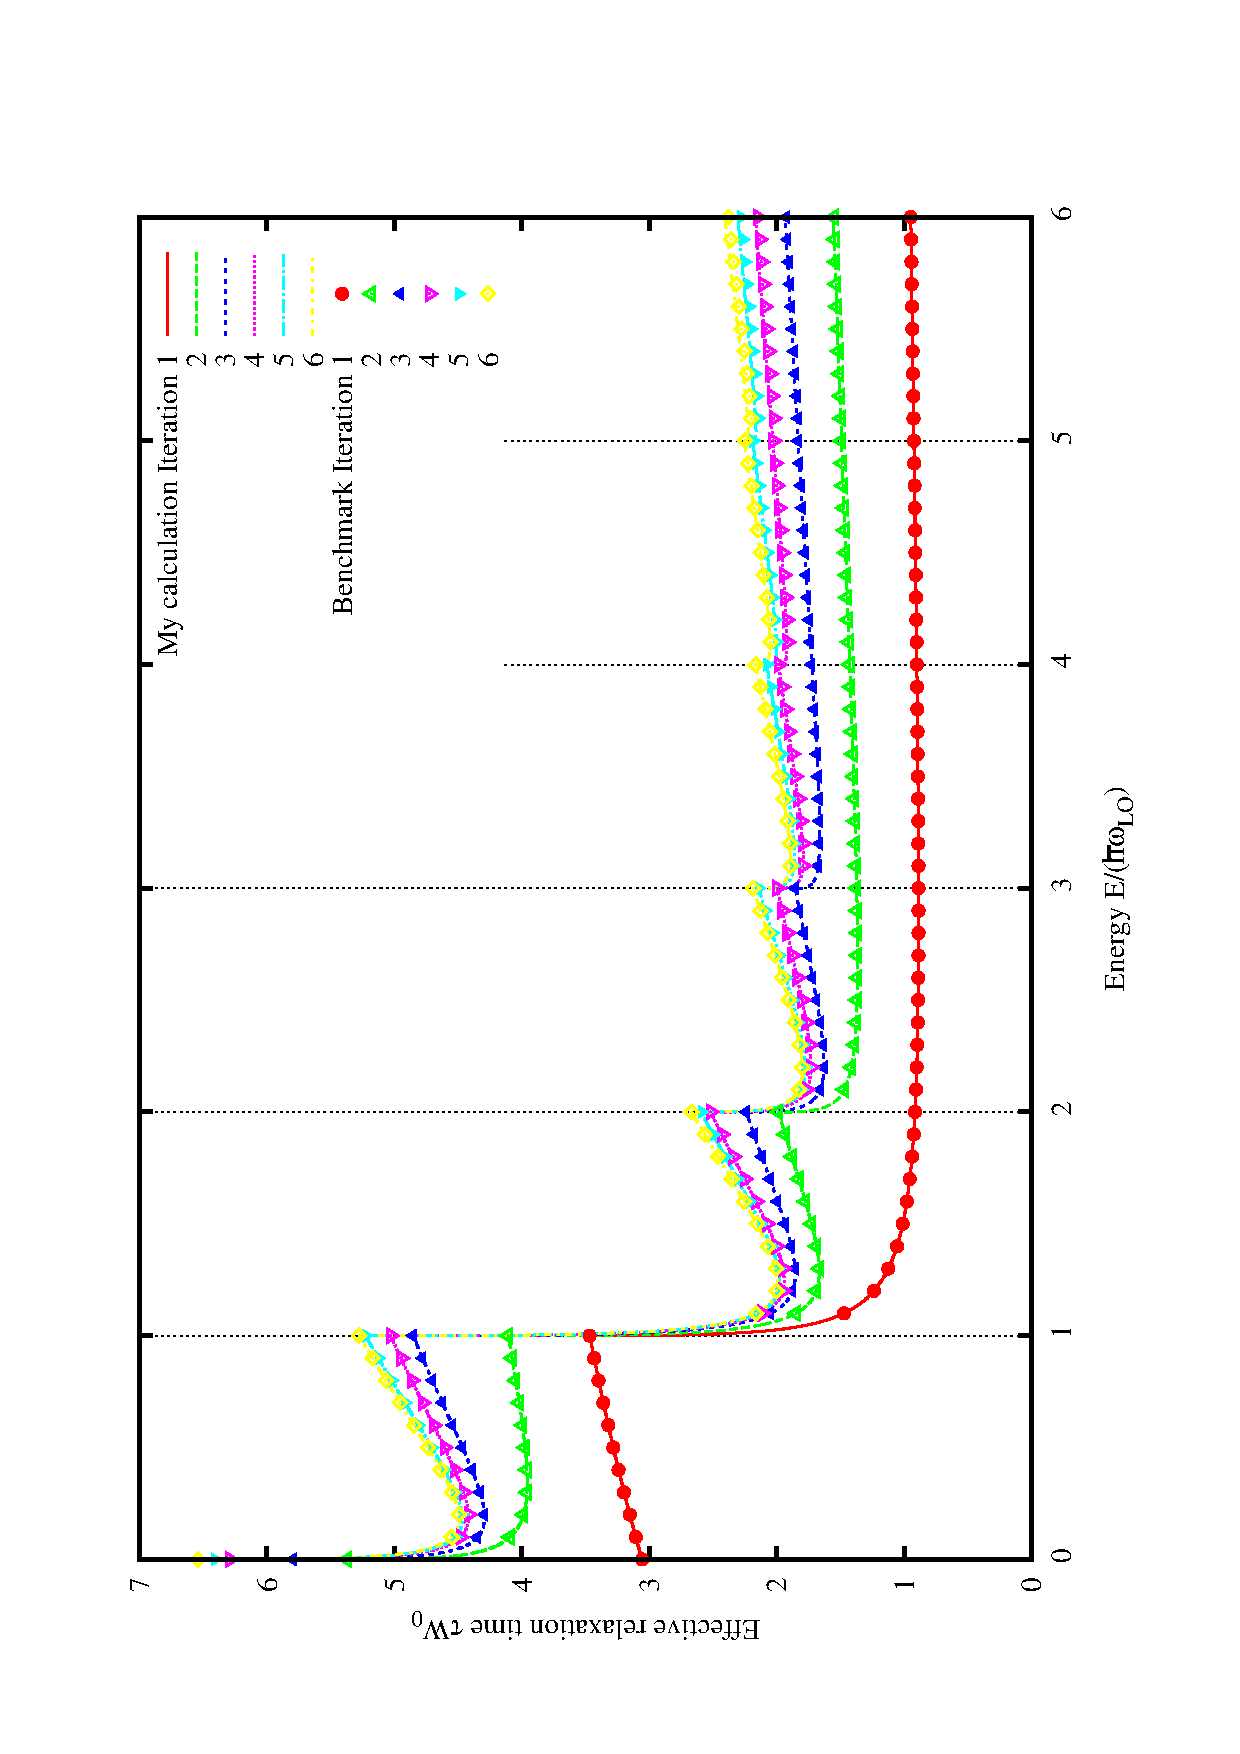
\includegraphics[width=\textwidth]{plots/tauLOiteration.pdf}
    %~/code/momentum_relaxation_rate/LOphonon/data
  \end{center}
  \caption{Effective momentum relaxation rate $\tau$ in units of $W_0^{-1}$, 
  with $W_0=(\frac{1}{\varepsilon_\infty}-\frac{1}{\varepsilon_0})\frac{2}{k_fa_0}\sqrt{\hbar\omega_{LO} E_F}$,
  see~\cite{Ridleyladdermethod}.
  The first six steps of the iteration are shown. A trend towards convergence
  is noticeable.
  The benchmarks have been calculated from~\cite{Martinscode}.
  It uses the Maxwell-Boltzmann distribution function.
  Our calculations use the Fermi-Dirac distribution function, which, however
  for GaAs at 300K and an electronic concentration of $10^{14}cm^{-3}$, at
  $\mu\beta \approx -8.4$ is far in the Maxwell Boltzmann regime.
  }
  \label{fig:tauLOiteration}
\end{figure}
%%%%%%%%%%%%%%%%%%%%%%%%%%%%%%%%%%%%%%%%%%%%%%%%%%%%
%%%%%%%%%%%%%%%%%%%%%%%%%%%%%%%%%%%
\paragraph*{Distribution function}%
%%%%%%%%%%%%%%%%%%%%%%%%%%%%%%%%%%%
The previous calculations yield the following corrections to the distribution function. 
We need to restrict the magnitude of the electric field for $f_1(K)$ to meet the requirement
$f_1(K)\ll f_0(K)$.

\paragraph*{Elastic solution for $K^2\gg W_{LO}$}
%%%%%%%%%%%%%%%%%%%%%%%%%%%%%%%%%%%%%%%%%%%%%%%%%%%%
\begin{equation}
  \begin{split}
E(K,\{z\})
&=- 
\left(\frac{1}{\varepsilon_\infty}-\frac{1}{\varepsilon_0}\right)
\frac{W_{LO}E_F}{n\hbar a_0k_F K}
    \times\\
&  \left\{~
%first integral, absorption
n_W
\frac{\sqrt{K^2+W_{LO}}}{K}
%second integral,emission 
+\Theta(K^2-W_{LO})
\left(n_W+1\right)
\frac{\sqrt{K^2-W_{LO}}}{K}
\right\}\\
&\stackrel{K^2\gg W_{LO}}{\to}
-\left(\frac{1}{\varepsilon_\infty}-\frac{1}{\varepsilon_0}\right)
\frac{W_{LO}E_F}{n\hbar a_0k_F K}
(2 n_{W_{LO}} +1)
\end{split}
  \label{eq:EK-LO}
\end{equation}

The elastic solution is then
$f_1(K)= A(K)/E(K)$, 
and the relaxation time $z(K) = E(K)^{-1}$, see \cite[page 388]{RID99}.
\alert{Strange handling of - sign, this shouldn't be there!}
%%%%%%%%%%%%%%%%%%%%%%%%%%%%%%%%%%%%%%%%%%%%%%%%%%%%
%%%%%%%%%%%%%%%%%%%%%%
\paragraph*{Mobility}%
%%%%%%%%%%%%%%%%%%%%%%
We can now calculate the mobility according to eq.~(\ref{eq:3d-mobility}).
Integrand
Convergence of mobility.


%%%%%%%%%%%%%%%%%%%%%%%%%%%%%%%%%%%%%%%%%%%%%%%%%%%%%%%%%%%%%%%%%%%%%%%%
\subsubsection{Example: Electron-plasmon scattering}
%%%%%%%%%%%%%%%%%%%%%%%%%%%%%%%%%%%%%%%%%%%%%%%%%%%%%%%%%%%%%%%%%%%%%%%%
%%%%%%%%%%%%%%%%%%%%%%%%%%%%%%%%%%%%%%%%%%%%
\begin{figure}[tb]
  \begin{center}
    \input{plots/plasma-cutoff}
  \end{center}
  \caption{Model plasmon dispersion}
  \label{fig:model-plasmon-dispersion}
\end{figure}
%%%%%%%%%%%%%%%%%%%%%%%%%%%%%%%%%%%%%%%%%%%%
We can model electron-plasmon scattering very similarly to 
electron phonon-scattering if we assume that the plasma frequency is
idependent of wave vector.
We simply need to set $W_{TO} = 0$ and $W_{LO}=W_{P}$, the dimensionless
plasma freqency, in all the equations of section~\ref{sec:LOphonon} above.

Plasmons can decay into pair excitations as soon as energy-momentum conservation allows it\footnote{citation needed}.
This is taken into account by introducing a cutoff wave-vector $Q_c$ with
\begin{equation}
  Q_C(Q_C+2) =W_P 
  \text{ or }
  Q_C = \sqrt{1+W_P} -1,
  \label{eq:Qcutoff}
\end{equation}
so that 
\begin{equation}
  W(Q) = W_P\Theta(Q-Q_C),
  \label{eq:cutoff-plasma-dispersion}
\end{equation}
see figure~\ref{fig:model-plasmon-dispersion}.

This means that, additionally to the changes described above, there will 
be a Heaviside step function $\Theta(Q-Q_C)$ in the integrands of all 
the integrals in eq.~(\ref{eq:BK-LO}) and eq.~(\ref{eq:DK-LO}).
Thus, we need to find out how large $Q_C$ is relative to the limits of 
those integrals. 
They are, in detail:
\begin{equation}
  Q^{em}_{\pm} = K \pm \sqrt{K^2 -W_P} 
  \text{ for emission, and }
  Q^{ab}_{\pm} = \sqrt{K^2 +W_P} \pm K
  \text{ for absorption.}
  \label{eq:Qpm}
\end{equation}
As $W_P$ >0, we have $Q_C < \sqrt{W_P}$, and therefore
$Q_C < Q_+^{ab}(K=0) \leq Q_+^{ab}$. 
Moreover, with the requirement $K>\sqrt{W_P}$ that needs to hold for 
emission, we get
$Q^{em}_+\geq Q^{em}_+(K_{min} =\sqrt{W_P}) = \sqrt{W_P} > Q_C$. 

Now for the lower limits. 
It is straightforward to see that both $Q^{ab}_-$ and $Q^{em}_-$ are 
monotonuously declining functions of $K$.
We will calculate $K_C^{\stackrel{ab}{em}}>0$ with 
$Q^{\stackrel{ab}{em}}(K_C^{\stackrel{ab}{em}}) =Q_C$.

It is obvoius that $K_C^{ab} =1$.
$K_C^{em} = \sqrt{1+W_P}$ is a little harder to discover, but is very easily verified.
In summary, we have 
%%%%%%%%%%%%%%%%%%%%%%%%%%%%%%%%%%%%%%%%%%%%%%%%%%%%
\begin{equation}
  \begin{aligned}
    K&\leq 1: 		&& Q_C\leq Q^{ab}_- < Q^{ab}_+\\
    K& >   1: 		&& Q^{ab}_-\leq Q_C < Q^{ab}_+\\
    K&\leq\sqrt{1+W_P}:	&& Q_C\leq Q^{em}_- < Q^{em}_+\\
    K& >\sqrt{1+W_P}: 	&& Q^{em}_-\leq Q_C < Q^{em}_+
  \end{aligned}
  \label{eq:plasmon-cutoff-limits}
\end{equation}
%%%%%%%%%%%%%%%%%%%%%%%%%%%%%%%%%%%%%%%%%%%%%%%%%%%%
and can now write evaluate the expressions $B(K)$ and $D(K,\{z\})$ for the cutoff-approximation to electron-plasmon scattering.
These expressions are eq.~(\ref{eq:BK-WP}) and ~(\ref{eq:DK-WP}) in appendix~\ref{app:electron-plasmon-scattering}.
%%%%%%%%%%%%%%%%%%%%%%%%%%%%%%%%%%%%%%%%%%%%%%%%%%%%%%%%%%%%%%%%%%%%%%%%%%%%%%%%%%%%%%%%%%%%%%%%%%%%%%%%
\appendix
\begin{landscape}
\chapter{Example: Electron-plasmon scattering}
\label{app:electron-plasmon-scattering}
%%%%%%%%%%%%%%%%%%%%%%%%%%%%%%%%%%%%%%%%%%%%%%%%%%%%
\begin{equation}
  \begin{aligned}
B(K) &=
\frac{1}{\varepsilon_\infty}
\frac{W_{P}E_F}{n\hbar a_0k_F K}
\frac{1}{1-f_0(K)}
\times\\ 
&\left\{
%first integral, absorption
\Theta(K-1)
n_W
\left[1-f_0\left(\sqrt{K^2+W_{P}}\right)\right] 
\ln\left(\frac{\sqrt{1+W_{P}}-1}{\sqrt{K^2+W_{P}}-K}\right)
\right.\\
%second integral, emission
&
\left.
+
\Theta(K-\sqrt{1+W_P})
\left(n_W+1\right)
\left[1-f_0\left(\sqrt{K^2-W_{P}}\right)\right] 
\ln\left(\frac{\sqrt{1+W_{P}}-1}{K-\sqrt{K^2-W_{P}}}\right)
\right\}
\end{aligned}
  \label{eq:BK-WP}
\end{equation}
%%%%%%%%%%%%%%%%%%%%%%%%%%%%%%%%%%%%%%%%%%%%%%%%%%%%
%%%%%%%%%%%%%%%%%%%%%%%%%%%%%%%%%%%%%%%%%%%%%%%%%%%%
\begin{equation}
  \begin{aligned}
&D(K,\{z\})
= 
 \frac{1}{\varepsilon_\infty}
\frac{W_{P}E_F}{n\hbar a_0k_F K}
\frac{1}{1-f_0(K)}
    \times \\
&\left\{~%
%first integral, absorption
 z\left(\sqrt{K^2+W_{P}}\right)
\Theta(K-1)
n_W
\left[1-f_0\left(\sqrt{K^2+W_{P}}\right)\right]
\left[
\left(1+\frac{W_{P}}{2K^2}\right)
\ln\left(\frac{Q_C}{Q_-^{ab}(K)}\right)
-\frac{Q_C^2-(Q_-^{ab}(K))^2}{4K^2}
\right]
\right.\\
%second integral,emission 
&+\left.
z\left(\sqrt{K^2-W_{P}}\right)
\Theta(K-\sqrt{1+W_P})
\left(n_W+1\right)
\left[1-f_0\left(\sqrt{K^2-W_{P}}\right)\right] 
\left[
\left(1-\frac{W_{P}}{2K^2}\right)
\ln\left(\frac{Q_C}{Q_-^{em}(K)}\right)
-\frac{Q_C^2-(Q_-^{em}(K))^2}{4K^2}
\right]
\right\}.
\end{aligned}
  \label{eq:DK-WP}
\end{equation}
%%%%%%%%%%%%%%%%%%%%%%%%%%%%%%%%%%%%%%%%%%%%%%%%%%%%
\end{landscape}

%%%%%%%%%%%%%%%%%%%%%%%%%%%%%%%%%%%%%%%%%%%%
%\clearpage
%%%%%%%%%%%%%%%%%%%%%%%%%%%%%%%%%%%%%%%%%%%%
%\section{Mermin collisional damping correction?}
%\section{T $>$0}
%\section{123-d}
%\section{Polar optical phonons}
%\section{$\varepsilon_{tot}=1+\sum \chi_i$ and resulting coupled modes}
%\section{Kim, Das, Senturia and Ridley and Stroscia and Fischetti approximations}
%\section{Im($\frac{1}{\epsilon}$) for a coupled system}
%\section{T $>$0}
%\section{123-d}
%%%%%%%%%%%%%%%%%%%%%%%%%%%%%%%%%%%%%%%%%%%%%%%%%%%%%%%%%%%%%%%%%%%
%%%%%%%%%%%%%%%%%%%%%%%%%%%%%%%%%%%%%%%%%%%%%%%%%%%%%%%%%%%%%%%%%%%
%\clearpage
%\appendix
%%%%%%%%%%%%%%%%%%%%%%%%%%%%%%%%%%%%%%%%%%%%%%%%%%%%%%%%%%%%%%%%%%
%\chapter{Degenerate limit parameterisation, $k_B T<< \mu$}
%\subsubsection{Why $\mu$ scaling?}
%In this parametrization, we only use explicitly use the chemical potential, and not the Fermi energy or wave vector for scaling.
%The advantage of this approach is that we need fewer physical concepts to capture the problem. 
%The disadvantag is that the chemical potential, and more the derivative ``chemical potential wave vector $k_\mu=\sqrt{\frac{2 m |\mu|}{\hbar^2}}$ is less intuitive than the Fermi wave vector.
%Moreover, the chemical potential can become zero and negative, which makes it less suitable for scaling anything with it.
%
%\subsubsection{Scaling}
%Next, the expression $F_0(v \pm \frac{\hbar k}{2 m})$ in the integrand of (\ref{eq:eps-wigner-poisson}) needs to be evaluated. 
%The argument of $\mathfrak{F}_0$, $\beta \left[ \mu -\frac{m}{2}\left(v \pm \frac{\hbar k}{2m}\right)^2\right]
%=\beta \left[ \mu - |\mu|\left(\frac{v}{v_\mu}\pm\frac{k}{2k_\mu}\right)^2\right]$,
%once one introduces $v_\mu=\sqrt{\frac{2|\mu|}{m}}$ and $k_\mu=\frac{\sqrt{2m|\mu|}}{\hbar}$,the Fermi velocity and wave vector at nonzero temperature.
%While these concepts only make sense for degenerate cases, i.e., where the chemical potential $\mu$ is positive, the formalism can be extended to $\mu<0$ by introducing the modulus.
%However, it has to be  kept in mind that the following formulae do not hold for $\mu=0$.
%
%With these parameters, the dielectric function reads
%\begin{equation}
%  \begin{split}
%  \varepsilon(k,\omega)=1-
%  \frac{1}{3}\frac{k_{TF}^2}{k^2}\frac{k_\mu}{k}\sqrt{\frac{\beta\mu}{\pi}}\frac{1}{\mathfrak{F}_\frac{1}{2}(\mu\beta)}
%  \int\limits_{\Gamma_L} \frac{d u}{u-\frac{\omega}{k v_\mu}} 
%  \left\{
%   \ln\left[ 1+\exp\left(\beta\mu- \beta|\mu|(u+\frac{k}{2k_\mu})^2 \right)\right]
%   \right. \\ \left.
%  -\ln\left[ 1+\exp\left(\beta\mu- \beta|\mu|(u-\frac{k}{2k_\mu})^2 \right)\right]
%  \right\}.
%  \end{split}
%  \label{eq:epsTnonzero}
%\end{equation}
%If we introduce the dimensionless prefactor 
%$A=
%  \frac{1}{3}\frac{k_{TF}^2}{k^2}\frac{k_\mu}{k}\sqrt{\frac{\beta\mu}{\pi}}\frac{1}{\mathfrak{F}_\frac{1}{2}(\mu\beta)}$
%wave vector 
%$b=\frac{k}{2k_\mu}$
%and phase velocity
%$c=\frac{\omega}{k v_\mu}$,
%the dielectric function 
%\begin{equation}
%  \varepsilon = 1-A 
%  \int\limits_{\Gamma_L} \frac{d u}{u-c} 
%  \left\lbrace
%   \ln \left\{  1+\exp\left(\beta\mu- \beta|\mu|(u+b)^2 \right) \right\}
%   -\ln \left\{ 1+\exp\left(\beta\mu- \beta|\mu|(u-b)^2 \right) \right\} 
%  \right\rbrace
%  \label{eq:epsTnonzeroshort}
%\end{equation}
%fits onto one line.
%Remember that $c=c_r+ic_i$ is a complex quantity, because $\omega$ is.
%
%\subsubsection{Real and imaginary part  of the dielectric function}
%The integration in eq.~(\ref{eq:epsTnonzero}) and eq.~(\ref{eq:epsTnonzeroshort}) is along the Landau contour $\Gamma_L$. 
%\paragraph*{Residue contribution}
%The contribution from the integral along the path below the pole of the dielectric function 
%eq.~(\ref{eq:epsTnonzeroshort}) at $u=c$ is
%  \begin{equation}
%    \varepsilon_{res}=-2\pi I \,A 
%  \left\lbrace
%   \ln \left\{  1+\exp\left(\beta\mu- \beta|\mu|(c+b)^2 \right) \right\}
%   -\ln \left\{ 1+\exp\left(\beta\mu- \beta|\mu|(c-b)^2 \right) \right\} 
%  \right\rbrace,
%    \label{eq:epsTnonzero_res}
%  \end{equation}
%  according to the Cauchy principal formula, see above.
%  This only holds if the logarithm is analytic between the real axis and and the pole.\\
%  CHECK LATER!
%\paragraph*{Contribution form integral along the real axis}
%The contribution to the integral from the integration along the real axis has the real part
%\begin{equation}
%   \varepsilon_r = 1-A 
%  \int\limits_{-\infty}^\infty du
%  \frac{u-c_r}{(u-c_r)^2+c_i^2} 
%   \ln
%   \left[
%   \frac{  1+\exp\left(\beta\mu- \beta|\mu|(u+b)^2 \right) }
%   { 1+\exp\left(\beta\mu- \beta|\mu|(u-b)^2 \right) } 
%   \right]
%  \label{eq:epsTnonzero_r}
%\end{equation}
%and the imaginary part
%\begin{equation}
%   \varepsilon_i = -A 
%  \int\limits_{-\infty}^\infty du
%  \frac{c_i}{(u-c_r)^2+c_i^2} 
%   \ln
%   \left[
%   \frac{  1+\exp\left(\beta\mu- \beta|\mu|(u+b)^2 \right) }
%   { 1+\exp\left(\beta\mu- \beta|\mu|(u-b)^2 \right) } 
%   \right].
%  \label{eq:epsTnonzero_i}
%\end{equation}
%Both integrals are well-defined as long as $c$ has a non-vanishing imaginary part. 
%If $c$ becomes real, $\varepsilon_i$ vanishes,
%but the integrand in the real part integral has a pole at $u=c_r$.
%
%\paragraph*{Evaluation of $\varepsilon_r$ for real frequencies}
%Let us investigate the integral in (\ref{eq:epsTnonzero_r}) for $ci=0$ more closely.
%If we introduce the integral 
%\begin{equation}
%  I_a(x)=\int\limits_{-\infty}^\infty \frac{du}{u} 
%  \ln\left[1+\exp\left(a- |a|(u+x)^2 \right)\right],
%  \label{eq:Int_mu_x}
%\end{equation}
%we can write
%\begin{equation}
%   \int\limits_{-\infty}^\infty 
%  \frac{d u}{u} 
%   \ln
%   \left[
%   \frac{  1+\exp\left(\beta\mu- \beta|\mu|(u+c_r+b)^2 \right) }
%   { 1+\exp\left(\beta\mu- \beta|\mu|(u+c_r-b)^2 \right) } 
%   \right]=I_{\mu\beta}(c_r+b) -I_{\mu\beta}(c_r -b).
%  \label{eq:epsTnonzero_realfrequency}
%\end{equation}
%Transforming $I_a(x)$ so that the integration is only over positive u yields
%\begin{equation}
%   I_a(x)=\int\limits_{0}^\infty \frac{du}{u} 
%  \ln\left[
%  \frac
%  { 1+\exp\left(a- |a|(u+x)^2 \right)}
%  { 1+\exp\left(a- |a|(u-x)^2 \right)}
%  \right].
%  \label{eq:Int_mu_x}
%\end{equation}
%It is easy to see that $I_a(x)$ is antisymmetric with respect to x.
%Moreover, according to L'Hospital's rule,
%\[
%\lim_{u \to 0}  i_a(u,x)=\lim_{u \to 0} \frac{1}{\frac{\partial}{\partial u} u}\frac{\partial}{\partial u}  \ln\left[
%  \frac
%  { 1+\exp\left(a- |a|(u+x)^2 \right)}
%  { 1+\exp\left(a- |a|(u-x)^2 \right)}
%  \right]
%  =-\frac{4|a|x}{ 1+\exp\left(-a + |a|x^2 \right)}
%\]
%its integrand  $i_a(u,x)$ doesn't become singular at $u=0$.
%
%Moreover, the integrand $i_a(u,x)$ decays exponentially for large u. 
%Let the Gaussian centered around x in $i_a(u,x)$ have decayed so that it's way smaller than ununity - for example at $u=x+\sqrt{\frac{a+2\ln10}{|a|}}$, the Gaussian would have fallen off to 0.01-
%a Taylor expansion of the logarithm in the integrand will yield
%$i_a(u,x)\approx \frac{1}{u}\exp(a-|a|(u-x)^2$.
%That means that tail of the integral for very large u converges.
%
%$I_a(x)$ will have to be calculated numerically and tabulated for every $a$ and $x$. 
%However, the assymtotic behaviour for large x can be calculated more easily.
%For $x\gg1$ , $e^{-2|a|ux} \ll e^{2|a|ux}$, so that 
%$I_a(x)\approx-\int\limits_{0}^\infty\;\frac{du}{u}\ln\left[1+\exp\left(a-|a|(u-x)^2\right)\right]$.
%If, moreover, the width of the gaussian is much smaller than x 
%- say $x\gg\sqrt{\ln(10)/|a|}$, the width where the Gaussian has fallen off to a tenth of its peak value -
%we can approximate further
%\[
%I_a(x)\approx -\frac{1}{x}\int\limits_{0}^\infty du 
%  \ln\left[ 1+\exp\left(a- |a|(u-x)^2 \right) \right]
%  =-\frac{2}{\sqrt{|a|}x}\int\limits_{0}^\infty du 
%  \ln\left[ 1+\exp\left(a-u^2\right) \right]. 
%\]
%The last expression has the advantage that it only constains an integral which is independent of x.
%\begin{figure}[ht]
%  \begin{center}
%    %\includegraphics{integral_a_x.pdf}
%    % GNUPLOT: LaTeX picture with Postscript
\begingroup
  \makeatletter
  \providecommand\color[2][]{%
    \GenericError{(gnuplot) \space\space\space\@spaces}{%
      Package color not loaded in conjunction with
      terminal option `colourtext'%
    }{See the gnuplot documentation for explanation.%
    }{Either use 'blacktext' in gnuplot or load the package
      color.sty in LaTeX.}%
    \renewcommand\color[2][]{}%
  }%
  \providecommand\includegraphics[2][]{%
    \GenericError{(gnuplot) \space\space\space\@spaces}{%
      Package graphicx or graphics not loaded%
    }{See the gnuplot documentation for explanation.%
    }{The gnuplot epslatex terminal needs graphicx.sty or graphics.sty.}%
    \renewcommand\includegraphics[2][]{}%
  }%
  \providecommand\rotatebox[2]{#2}%
  \@ifundefined{ifGPcolor}{%
    \newif\ifGPcolor
    \GPcolortrue
  }{}%
  \@ifundefined{ifGPblacktext}{%
    \newif\ifGPblacktext
    \GPblacktexttrue
  }{}%
  % define a \g@addto@macro without @ in the name:
  \let\gplgaddtomacro\g@addto@macro
  % define empty templates for all commands taking text:
  \gdef\gplbacktext{}%
  \gdef\gplfronttext{}%
  \makeatother
  \ifGPblacktext
    % no textcolor at all
    \def\colorrgb#1{}%
    \def\colorgray#1{}%
  \else
    % gray or color?
    \ifGPcolor
      \def\colorrgb#1{\color[rgb]{#1}}%
      \def\colorgray#1{\color[gray]{#1}}%
      \expandafter\def\csname LTw\endcsname{\color{white}}%
      \expandafter\def\csname LTb\endcsname{\color{black}}%
      \expandafter\def\csname LTa\endcsname{\color{black}}%
      \expandafter\def\csname LT0\endcsname{\color[rgb]{1,0,0}}%
      \expandafter\def\csname LT1\endcsname{\color[rgb]{0,1,0}}%
      \expandafter\def\csname LT2\endcsname{\color[rgb]{0,0,1}}%
      \expandafter\def\csname LT3\endcsname{\color[rgb]{1,0,1}}%
      \expandafter\def\csname LT4\endcsname{\color[rgb]{0,1,1}}%
      \expandafter\def\csname LT5\endcsname{\color[rgb]{1,1,0}}%
      \expandafter\def\csname LT6\endcsname{\color[rgb]{0,0,0}}%
      \expandafter\def\csname LT7\endcsname{\color[rgb]{1,0.3,0}}%
      \expandafter\def\csname LT8\endcsname{\color[rgb]{0.5,0.5,0.5}}%
    \else
      % gray
      \def\colorrgb#1{\color{black}}%
      \def\colorgray#1{\color[gray]{#1}}%
      \expandafter\def\csname LTw\endcsname{\color{white}}%
      \expandafter\def\csname LTb\endcsname{\color{black}}%
      \expandafter\def\csname LTa\endcsname{\color{black}}%
      \expandafter\def\csname LT0\endcsname{\color{black}}%
      \expandafter\def\csname LT1\endcsname{\color{black}}%
      \expandafter\def\csname LT2\endcsname{\color{black}}%
      \expandafter\def\csname LT3\endcsname{\color{black}}%
      \expandafter\def\csname LT4\endcsname{\color{black}}%
      \expandafter\def\csname LT5\endcsname{\color{black}}%
      \expandafter\def\csname LT6\endcsname{\color{black}}%
      \expandafter\def\csname LT7\endcsname{\color{black}}%
      \expandafter\def\csname LT8\endcsname{\color{black}}%
    \fi
  \fi
  \setlength{\unitlength}{0.0500bp}%
  \begin{picture}(7200.00,5040.00)%
    \gplgaddtomacro\gplbacktext{%
      \csname LTb\endcsname%
      \put(1760,1024){\makebox(0,0)[r]{\strut{} 0.001}}%
      \put(1760,1797){\makebox(0,0)[r]{\strut{} 0.01}}%
      \put(1760,2569){\makebox(0,0)[r]{\strut{} 0.1}}%
      \put(1760,3342){\makebox(0,0)[r]{\strut{} 1}}%
      \put(1760,4115){\makebox(0,0)[r]{\strut{} 10}}%
      \put(1952,704){\makebox(0,0){\strut{} 0.01}}%
      \put(3319,704){\makebox(0,0){\strut{} 0.1}}%
      \put(4685,704){\makebox(0,0){\strut{} 1}}%
      \put(6052,704){\makebox(0,0){\strut{} 10}}%
      \put(256,2839){\rotatebox{-270}{\makebox(0,0){\strut{}$I_a(x)$}}}%
      \put(6782,2839){\rotatebox{-270}{\makebox(0,0){\strut{}}}}%
      \put(4207,224){\makebox(0,0){\strut{}x}}%
      \put(4207,4495){\makebox(0,0){\strut{}}}%
      \put(4207,4494){\makebox(0,0){\strut{}}}%
      \put(416,160){\makebox(0,0)[l]{\strut{}}}%
    }%
    \gplgaddtomacro\gplfronttext{%
      \csname LTb\endcsname%
      \put(5056,4432){\makebox(0,0)[r]{\strut{}Approximation $x\gg1$}}%
      \csname LTb\endcsname%
      \put(5056,4112){\makebox(0,0)[r]{\strut{}Numerical evaluation}}%
    }%
    \gplbacktext
    \put(0,0){\includegraphics{plots/integralax.pdf}}%
    \gplfronttext
  \end{picture}%
\endgroup

%  \end{center}
%  \caption{Plot of $I_a(x)$ for $a \in \{-5,-1,1,5,10\}$ from bottom to top. Also plotted are the approximations for large x for the same values of $a$.}
%  \label{fig:integral_a_x}
%\end{figure}
%Figure \ref{fig:integral_a_x} shows the numerically calculated $I_a(x)$ for several choices of a.
%%%%%%%%%%%%%%%%%%%%%%%%%%%%%%%%%%%%%%%%%%%%%%%%%%%%%%%%%%%%%%%%%%%
%
%
%%%%%%%%%%%%%%%%%%%%%%%%%%%%%%%%%%%%%%%%%%%%%%%%%%%%%%%%%%%%%%%%%%%
\clearpage
%\chapter{References}
%\nocite{*}
%\bibliographystyle{poster} 
\bibliographystyle{unsrtnat} 
\bibliography{landaurefs,references}
%\bibliography{references}%for at home
%%%%%%%%%%%%%%%%%%%%%%
\end{document}
